	% !TEX root = applied-math.tex


\chapter{Basics of Linear Algebra}

\section{Solving Linear Systems} \label{sect:linear:syst}

We start this section with three examples of linear systems.  One is about a bi\-ath\-lon with running and biking legs, a traffic flow model and finally an example from Chemistry.  Examples of linear systems are found from every mathematical subfield and every science.  

\begin{example} \label{ex:biathlon}
Travis runs 6 mph and bikes 18 mph in a race with two events.  If the course is 29 miles long and it takes him 2 hours and 10 minutes to complete the race,  how long is each segment?

\solution

In this case, we need to know how long each segment is.  There are two legs to the race, so we will let
\begin{align*}
x_1 & = \text{number of miles for the run,}\\
x_2 & = \text{number of miles for the bike.}
\end{align*}


The equations come from three statements in the problem above.  First, we know that the total course is 29 miles long or
%
\begin{align*}
	x_1+x_2&=29.
\end{align*}

The remaining equation arises from the time it takes Travis to complete the race.  In general recall the relationship between speed (a rate), distance and time is
\begin{align*}
	\text{speed} & = \frac{\text{distance}}{\text{time}}
\end{align*}
or solving for time, 
\begin{align*}
	\text{time} & =\frac{\text{distance}}{\text{rate}}
\end{align*}

For example, the time it takes Travis to finish the running leg is $x_1/6$.  The total time it takes Travis to finish the race is 
%
\begin{align*}
\frac{x_1}{6} + \frac{x_2}{18}  & = 2+ \frac{10}{60} = \frac{13}{6}, \\
\end{align*}
%
so the linear system is
%
\begin{align*}
x_1+x_2&=29, \\
\frac{x_1}{6} + \frac{x_2}{18} & =\frac{13}{6}.\\
\end{align*}

\end{example}

The next example examines the traffic flow in a very limited part of a city (Boston in this case).  

\begin{example} \label{ex:traffic}

A simple model of traffic flow can be represented by the following graph:

\begin{center}
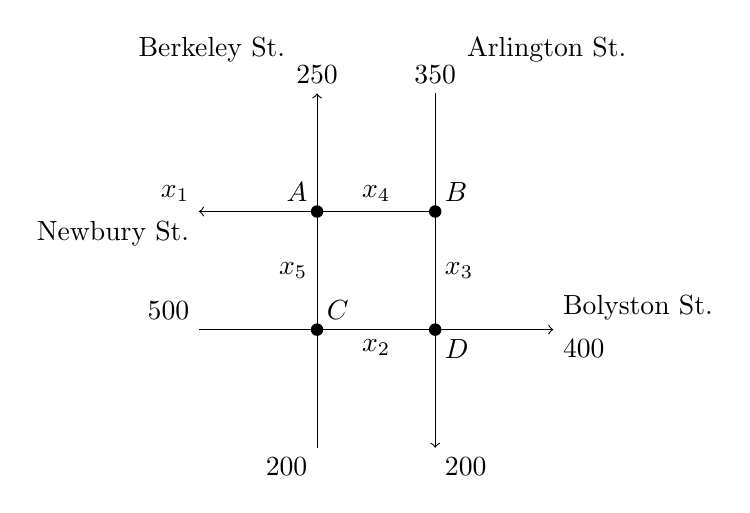
\begin{tikzpicture}[scale=1.5]

\draw[<-] (0,1) -- (2,1) node [at start,below left] {Newbury St.};
\draw[->] (0,0) -- (3,0) node [at end,above right] {Bolyston St.} ;
\draw[<-] (1,2) -- (1,-1) node [at start,above left=5pt+3pt] {Berkeley St.};
\draw[<-] (2,-1) -- (2,2) node [at end,above right=5pt+3pt] {Arlington St.} ;

\draw (3,0) node [below right] {400};
\draw (2,-1) node [below right] {200};
\draw (0,0) node [above left] {500}; 
\draw (1,-1) node [below left] {200}; 
\draw (0,1) node [above left] {$x_1$};
\draw (1,2) node [above] {250}; 
\draw (2,2) node [above] {350}; 

\draw (1.5,0) node [below] {$x_2$};
\draw (2,0.5) node [right] {$x_3$};
\draw (1.5,1) node [above] {$x_4$};
\draw (1,0.5) node [left] {$x_5$}; 

\fill (1,1) circle[radius=1.5pt] node [above left] {$A$};
\fill (2,1) circle[radius=1.5pt] node [above right] {$B$};
\fill (1,0) circle[radius=1.5pt] node [above right] {$C$};
\fill (2,0) circle[radius=1.5pt] node [below right] {$D$};

\end{tikzpicture}
\end{center}
where the arrows denote the direction of traffic flow (all of these streets are one-way) and the numbers represent the numbers of cars driving down the street in a given time period.  The letters $A$ through $D$ will be the names of the intersections.   

And a mathematical model can be written down by making sure that the total number of cars that go into an intersection balances with the number of cars exiting.  In this case, we have:
%
\begin{align*}
x_4 + x_5 & = x_1 + 250\\ 
350 & = x_3 + x_4 \\
700 & = x_2 + x_5 \\
x_3 + x_2 & =  600 \\
\end{align*}
for intersections $A$, $B$, $C$ and $D$ respectively. 
\end{example}

Linear equations exist in many different fields, especially the sciences.  The following comes from Chemistry in which a chemical equation is found by balancing the number of atoms in the equation on both sides.  

\begin{example} \label{ex:hydrazine}
Hydrazine ($N_2H_4$)  is an important nitrogen-based com\-pound.  A chemical reaction to produce it from ammonia and hydrogen peroxide is given by
%
\begin{align*}
k_1 NH_3 + k_2 H_2O_2 \rightarrow k_3 N_2 H_4 + k_4 H_2 O 
\end{align*}
%
The values of $k_1, k_2, k_3$ and $k_4$ can be found by solving the following linear system which balances the number of nitrogen (N), hydrogen (H) and oxygen (O) atoms in the reaction or
%
\begin{align*}
k_1 & = 2k_3, \\
3k_1 + 2k_2 & = 4k_3 + 2k_4, \\
2k_2 & = k_4.
\end{align*}
\end{example}

With examples of linear algebra presented, we next move to a method of solution. 

\subsection{Gauss's Method}

We now seek a method to solve the above linear systems (and any linear system).  Gauss' method and variations of it are the standard ways that all large linear systems are solved presently.   We first start with defining a few important terms:
\begin{definition}  ~ 

\begin{itemize}
\item
A \textbf{linear combination} of $x_1, x_2, x_3, \ldots, x_n$ has the form
%
\begin{align*}
a_1 x_1 + a_2 x_2 + \cdots + a_n x_n, 
\end{align*}
where the numbers $a_1, a_2, \ldots, a_n \in \mathbb{R}$ are the combinations coefficients.  

\item A \textbf{linear equation} has the form
%
\begin{align}
a_1 x_1 + a_2 x_2 + \cdots + a_n x_n & = b 
\label{eq:def:lin:eq}
\end{align}
where $b \in \mathbb{R}$ is a constant.  
\item The $n$-tuple $(s_1,s_2,\ldots,s_n)$ \textbf{satisfies} or is a \text{solution} of (\ref{eq:def:lin:eq}) if this point satisfies (\ref{eq:def:lin:eq}) or 
%
\begin{align*}
a_1 s_1 + a_2 s_2 + \cdots + a_n s_n & = b
\end{align*}
\item A \textbf{system of linear equations} or \text{linear system} is a set of linear equations:
%
\begin{align}
\begin{split}
a_{1,1} x_1 + a_{1,2} x_2 + \cdots + a_{1,n} x_n & = b_1 , \\
a_{2,1} x_1 + a_{2,2} x_2 + \cdots + a_{2,n} x_n & = b_2, \\
\vdots & = \vdots \\
a_{m,1} x_1 + a_{m,2} x_2 + \cdots + a_{m,n} x_n & = b_m, \\
\end{split} \label{eq:def:lin:sys}
\end{align}
and this linear system has $m$ equations and $n$ unknowns (variables).  
\item The $n$-tuple $(s_1,s_2,\ldots,s_n)$ \textbf{satisfies} or is a \text{solution} of (\ref{eq:def:lin:sys}) if this point satisfies every equation of (\ref{eq:def:lin:sys}).  
\end{itemize}

\end{definition}

\begin{example}
The following are linear equations:
%
\begin{align*}
2x_1 + 3x_2 & = 6, & x_1 -x_2+x_3-x_4 & = 10, \\
 10x_1 - x_3 + 5x_5 & = 9,  & \sum_{i=1}^{10} i x_i & = 0 
\end{align*}
and the following are not:
%
\begin{align*}
x_1^2+x_2 & = 6, & x_1x_2 + x_3 & = 5, \\
\frac{x_1+x_2}{x_3} & = 6, & \sin(x+y) &= z 
\end{align*}
\end{example}

The next two examples give a way to determine if a point or $n$-tuple is a solution to a linear system.  

\vspace{1in}

\begin{example}
Show that the point $(2,3)$ is a solution of  the linear system:
%
\begin{align*}
3x_1 - x_2 & = 3 \\
2x_1 + 4x_2 & = 16
\end{align*}

\solution

Substitute $x_1=2$ and $x_2=3$ into both equations and check. 
\begin{align*}
3(2) - 3 & = 3, \\
2(2) + 4(3) & = 16. 
\end{align*}
Since each equation is satisfied at the point $(2,3)$ is a solution to the linear system.  

\end{example}

\phantom{Here's some text}



\phantom{Here's some text}

\begin{example}
Recall that the linear system in Example \ref{ex:hydrazine} can be written:
\begin{align*}
k_1 \phantom{+2k_2}- 2k_3\phantom{+2k_4} & = 0, \\
2k_2 + 2k_3 -2k_4 & = 0, \\
2k_2 \phantom{+2x_3}- k_4 & = 0,
\end{align*}

Is $(8,4,4,8)$ a solution to this linear system?  Is $(4,2,2,4)$? \\  Is $(6,1,3,2)$?

\solution

For $(8,4,4,8)$, we need to substitute this point in and check all the equations:
%
\begin{align*}
8-2(4) & = 0 \\
2(4)+2(4)-2(8) & = 8+8-16 = 0 \\
2(4)-8 & = 8-8 = 0  
\end{align*}
so it is a solution. 

For $(4,2,2,4)$, again check all of the equations:
%
\begin{align*}
4-2(2) & = 0, \\
3(4)+2(2)-4(2)-2(4) & = 12+4-8-8=0, \\
2(2)-4& = 0
\end{align*}
so this is also a solution.  


For $(6,1,3,2)$, we substitute this into the equation:
%
\begin{align*}
6-2(3) & = 0 \\
3(6)+2(1)-4(3)-2(2) & = 18+2-12-4 = 4 \neq 0. \\
2(1) - 2 & = 0 
\end{align*}
and it satisfies 2 of the equations, but not all, so this is not a solution.  

\end{example}


\subsection{Solving a Linear System with Gauss' Method} 

The following example shows how we can solve a linear system with a technique called \textbf{Gauss' Method}.  

\begin{align*}
x -2y + 3z  &= 6, \\
2x + 2 y\phantom{+2z} &= 6, \\
-3x \phantom{+2y}+\phantom{3} z  &= 0.
\end{align*}

If one equation had only one variable, it would be quite easy to find the solution to that equation.  The following steps will result in such a system.  For example, if the first equation is multiplied by $-2$ and added to the second equation and the second equation is replaced (which we denote with $-2R_1+R_2 \rightarrow R_2$), then the above equations are replaced with 
%
\begin{align*}
&&x -2y + 3z  &= 6, \\
-2R_1+R_2 \rightarrow R_2&&6 y-6z &= -6, \\
&&-3x \phantom{+2y}+\phantom{3} z  &= 0.
\end{align*}
Next, we'd like to get rid of the $x$ term in the 3rd equation.  We can do that by multiplying the first equation by 3 and adding to the 3rd and writing down this operation as well we get:
%
\begin{align*}
&&x -2y + \phantom{1}3z  &= 6, \\
3R_1+R_3 \rightarrow R_3 && 6 y-\phantom{1}6z &= -6, \\
&&-6y+10z & = 18. 
\end{align*}
Next we will eliminate the $y$ term in the 3rd equation.  We can do that by adding equations 2 and 3 and putting the result in equation 3. 
\begin{align}
&&x -2y + 3z  &= 6, \notag \\
R_2+R_3 \rightarrow R_3 &&  6 y-6z &= -6,  \label{eq:gauss:method} \\
&& 4z & = 12.  \notag
\end{align}

At this point we can solve for $z$ in the third equation of (\ref{eq:gauss:method}) to get $z=3$.  From this, plug in $z=3$ into the second equation of (\ref{eq:gauss:method}) to get
%
\begin{align*}
6y -6(3) & = -6  \\
6y & = 12 \\
y & = 2 
\end{align*}
and finally we can use $z=3$ and $y=2$ to substitute into the first equation of (\ref{eq:gauss:method}) to get 
%
\begin{align*}
x-2(2)+3(3)& = 6 \\
x-4+9& = 6 \\
x & = 1 
\end{align*}
therefore, $x=1$.  The point $(1,2,3)$ is a solution to linear system.    Because this is the only point that satisfies all equations, this point is \textbf{unique}.  We will also use the terminology triple to describe $(1,2,3)$.  


\begin{theorem}[Gauss's Method] \label{thm:gauss:method}
If a linear system ($A$) is changed into a second linear system ($B$) by one of the following operations:
\begin{enumerate}
\item Two equations of the linear system are swapped,
\item An equation is multiplied by a nonzero number,
\item An equation is replaced by the sum of itself and a multiple of another equation, 
\end{enumerate}
then linear systems ($A$) and ($B$) have the same set of solutions.  
\end{theorem}


\begin{proof}
We will consider only the first operation in this proof.  Let's assume that we swap equations $i$ and $j$, thus system ($A$),  
\begin{align*}
a_{1,1} x_1 + a_{1,2} x_2 + \cdots + a_{1,n} x_n & = b_1 , \\
a_{2,1} x_1 + a_{2,2} x_2 + \cdots + a_{2,n} x_n & = b_2, \\
\vdots \qquad \qquad &  \vdots  \\
a_{i,1} x_1 + a_{i,2} x_2 + \cdots + a_{i,n} x_n & = b_i, \\
\vdots \qquad \qquad &  \vdots  \\
a_{j,1} x_1 + a_{j,2} x_2 + \cdots + a_{j,n} x_n & = b_j, \\
\vdots \qquad \qquad &  \vdots  \\
a_{m,1} x_1 + a_{m,2} x_2 + \cdots + a_{m,n} x_n & = b_m, \\
\end{align*}
is transformed to 
\begin{align*}
a_{1,1} x_1 + a_{1,2} x_2 + \cdots + a_{1,n} x_n & = b_1 , \\
a_{2,1} x_1 + a_{2,2} x_2 + \cdots + a_{2,n} x_n & = b_2, \\
\vdots \qquad \qquad &  \vdots  \\
a_{j,1} x_1 + a_{j,2} x_2 + \cdots + a_{j,n} x_n & = b_j, \\
\vdots \qquad \qquad &  \vdots  \\
a_{i,1} x_1 + a_{i,2} x_2 + \cdots + a_{i,n} x_n & = b_i, \\
\vdots \qquad \qquad &  \vdots  \\
a_{m,1} x_1 + a_{m,2} x_2 + \cdots + a_{m,n} x_n & = b_m, \\
\end{align*}

Let $(s_1,s_2, \ldots, s_n)$ be a solution of ($A$) if it exists and note it may be one of many $n$-tuples in the solution.  Thus it satisfies each equation of linear system ($A$).  Since the exact same equations are in ($B$) in just a different order, $(s_1,s_2,\ldots,s_n)$ is a solution to ($B$).   If there is more than one $n$-tuple in the solution to ($A$), repeat this for every one.  If there is no solution to ($A$), then there will be no solution to ($B$) since it is the same set of equations.  

Proof of \#2 and \#3 above are quite similar and are not shown.  
\end{proof}


\begin{definition}
The three operations in theorem \ref{thm:gauss:method} are called the \textbf{elementary reduction operations} or \textbf{elementary row operations} or \textbf{Gaussian operations} of a linear system.  
\end{definition}

\pagebreak

\begin{Boxed*}
Although Gauss' Method is very flexible, generally, one tries to eliminate all $x_1$ terms in all equations below equation 1, $x_2$ terms in all equations below equation 2 and so on.  
\end{Boxed*}


\subsubsection{A fourth Row Operation}

Another handy row operation is that of replacing a row with linear combination of itself and another row.  In general this is
%
\begin{align*}
c_i R_i + c_j R_j \rightarrow R_j
\end{align*}

Since this is a combination of two row operations together, we will use it, however, not consider it a separate (fourth) row operation.  



\begin{example} \label{ex:solve:linear:syst}
Use the strategy above to solve:
%
\begin{align*}
4x_1 \phantom{+3x_2}- x_3 & = 0, \\
x_1+3x_2 +2x_3 & = 3, \\
3x_2 + 5x_3 & = 14. 
\end{align*}


\solution

We first try to eliminate the $x_1$ term in the 2nd row.  We can accomplish this with
%
\begin{align*}
&&4x_1  \phantom{+3x_2}-\phantom{9}x_3 & = 0, \\
-R_1+4R_2 \rightarrow R_2 && 12x_2 +9x_3 & = 12, \\
&&3x_2 + 5x_3 & = 14. 
\end{align*}

Lastly, we try to eliminate the $x_2$ term in the 3rd equation with 
%
\begin{align*}
&&4x_1  \phantom{+3x_2}- \phantom{9}x_3 & = 0, \\
-R_2+4R_3 \rightarrow R_3 && 12x_2 +9x_3 & = 12, \\
&& 11x_3 & =  44
\end{align*}

Now at this point, we can solve for $x_3$, then $x_2$, then $x_1$ in a method called \textbf{back substitution}. 

\begin{align*}
11 x_3 & = 44 \\
x_3 & = 4 
\end{align*}
then substitute into the second equation, 
%
\begin{align*}
12x_2 + 9(4) & = 12 \\
12 x_2 & = 12-36=-24 \\
x_2 & = -2 
\end{align*}
and finally into the first equation, 
%
\begin{align*}
4x_1 - 4 & = 0 \\
4x_1 & = 4 \\
x_1 & = 1. 
\end{align*}
So the solution is $(1,-2,4)$.    Again, because there is only one solution to the equation $11x_3=44$, there is only one value for $x_3$, hence only one value for $x_2$ and only one values for $x_1$, so this solution is unique.  
\end{example}

\phantom{Here's some text}

\begin{example}
Solve the linear system for the biathlon race in example \ref{ex:biathlon}

\begin{align*}
x_1+x_2&=29, \\
\frac{x_1}{6} + \frac{x_2}{18} & =\frac{13}{6}, \\
\end{align*}

\solution

First to make life easier, let's multiple the 2nd equation by 18 to rid the fractions. 
%
\begin{align*}
18 R_2 \rightarrow R_2& \qquad
\begin{split}
x_1+x_2&=29, \\
3x_1 + x_2 & = 39, 
\end{split}  \intertext{Then we eliminate the $x$ in the 2nd equation by doing the following step,}
-3R_1 + R_2 \rightarrow R_2& \qquad
\begin{split}
x_1+x_2&=29, \\
 -2x_2 & = -48, 
\end{split}  
\end{align*}
and at this point, we can solve for $x_2$ in the last equation using back substitution.  $x_2=24$ and then 
%
\begin{align*}
x_1 + 24 & = 29 \intertext{therefore,}
x_1 & = 5
\end{align*}
So the running part of the race is 5 miles and the biking is 24 miles.  

\end{example}

\subsection{Echelon Form}

Notice that the strategy laid out above gets the linear system in a nice form for solving for all variables using back substitution.  We will now explicitly state what this nice form is. 

\begin{definition} \label{def:echelon:form}
In each equation of a linear system, the first variable with a non-zero coefficient is called the \textbf{leading variable}.  A system is in \textbf{echelon form} if each leading variable is to the right  of the leading variable of the equation above it (except the first equation). 
\end{definition}

In the definition above, it's important that there is some order to the variables.  If the variables are $x_1, x_2, \ldots$, then ``to the right'' means that there is a larger subscript.   If the variables are $x,y,z,\ldots$, the to the right is just after lexicographically.  


\begin{example} 

Show that  the linear system in the example above:
%
\begin{align*}
4x_1\phantom{+11x_3} -\phantom{9} x_3 & = 0, \\
 12x_2 +9x_3 & = 12, \\
11x_3 & =  44
\end{align*}
is in echelon form.  

\solution

Note that the leading variable in equation 1 is $x_1$, the leading variable in equation 2 is $x_2$ and the leading variable in equation 3 is $x_3$.  Each leading variable in each successive row is to the right of the one above. 

\end{example}

The next example determines if the system is in echelon form. 

\pagebreak

\begin{example}  \label{eq:echelon:form:3by5}
Is 
%
\begin{align*}
x_1\phantom{+2x_3} + 3x_3 -9 x_4 + 11 x_5 & = 14, \\
2x_3 \phantom{-9x_4} +\phantom{1} 4x_5 & = 10, \\
3x_5 & = 27,
\end{align*}
in echelon form? 

\solution

Yes, the leading variable in equation 1 is $x_1$, the leading variable in equation 2 is $x_3$ which is to the right of $x_1$ and the leading variable in equation 3 is $x_5$, which is to the right of $x_3$.    
\end{example}

\begin{example}
Is the system 
%
\begin{align*}  %(-3,4)
3x_1 + 4 x_2 & = 7, \\
2x_1 -x_2 & = -10, \\
2x_2 & = 8 
\end{align*}
in echelon form: 

\solution

No,  the leading variables in both equation 1 and 2 are $x_1$.  

\end{example}


Let's look more carefully at the last example.  It is not in echelon form, but let's put it in echelon form and write down a solution.  


\begin{align*}  %(-3,4)
\begin{split}
3x_1 + 4 x_2 & = 7, \\
2x_1 -x_2 & = -10, \\
2x_2 & = 8 
\end{split} \intertext{Eliminate $x_1$ in the 2nd equation by doing the following: }
-2R_1+3R_2 \rightarrow R_2, \qquad
\begin{split}
3x_1 + 4 x_2 & = 7, \\
 -11x_2 & = -44, \\
2x_2 & = 8 
\end{split}\intertext{then eliminate $x_2$ in the third equation}
2R_2 +11 R_3 \rightarrow R_3 \qquad
\begin{split}
3x_1 + 4 x_2 & = 7, \\
 -11x_2 & = -44, \\
0x_2 & = 0,  
\end{split}\\
\end{align*}
Note that the last equation in the last linear system contains no information.  zero equals zero.  We all knew that before. We ignore that equation.  The 2nd equation can be solved to yield $x_2=4$ and substituting into the first equation, 
%
\begin{align*}
3x_1 + 4(4) & = 7, && \text{or} \\ 
3x_1 & = -9, &&\text{or} \\
x_1 & = -3.  
\end{align*}
so the solution is $(-3,4)$.  


In comparison to the last example, consider the following very similar example:
\begin{align*}  %(-3,4)
\begin{split}
3x_1 + 4 x_2 & = 7, \\
2x_1 -x_2 & = -10, \\
3x_2 & = 6 
\end{split}\\[10pt]
-2R_1+3R_2 \rightarrow R_2, \qquad
\begin{split}
3x_1 + 4 x_2 & = 7, \\
 -11x_2 & = -44, \\
3x_2 & = 6,  
\end{split}\\[10pt]
3R_2+11R_3 \rightarrow R_3, \qquad
\begin{split}
3x_1 + 4 x_2 & = 7, \\
 -11x_2 & = -44, \\
0x_2 & = -66,  
\end{split}
\end{align*}

And note in this case, that the last equation says $0=-66$, which is not true.  Therefore, this means that there is no solution.  This is in contrast to the the previous example, which did have a solution.  


\subsubsection{Are there only unique and no solutions?}

In the last example of this section, we will see that we can have many solutions to a linear system.  If we have the following linear system already in echelon form:
%
\begin{align*}
x_1\phantom{+2x2} -2x_3\phantom{+x_4} & = 0, \\
2x_2 +2x_3 -2x_4 & = 0, \\
-2x_3 + x_4 & = 0, 
\end{align*}

Notice that since there are 4 variables and 3 equations, that there is no way to get a solution for $x_4$ by itself (or any of the other 3 variables).  This has many (actually infinitely many) solutions.  For example $(0,0,0,0)$ is one as well as $(2,1,1,2)$ and $(-5,-5/2,-5/2,-5)$.  We will explore this is much more detail later.  

\subsection{Describing the Solution Set}

So far we have seen linear system with solution sets with different number of elements.  The \emph{no solution} means that the solution set is empty, the \emph{unique solution} means that there is one element in the set.  But we haven't seen the \emph{many solutions} and how do we represent that.  We explore that here in this section. 

For example, if we reduce the linear system: \label{ex:many:solutions}
%
\begin{align*}
\begin{split}
x\phantom{+2y} + 2z & = -6 \\
2x-y\phantom{+3z}& = 1 \\
y+4z& = -13
\end{split} \\[12pt]
-2R_1+R_2 \rightarrow R_2 \qquad
\begin{split}
x\phantom{+2y} + 2z & = -6 \\
-y-4z& = 13 \\
y+4z& = -13
\end{split} \\[12pt]
R_2 + 2R_3 \rightarrow R_3 \qquad
\begin{split}
x\phantom{+2y} + 2z & = -6 \\
-y -4z & = 13 \\
0 & = 0 
\end{split} \\[12pt]
\end{align*}

As discussed above, this linear system has more that one solution.  Therefore it is the set of points that satisfy every one of the original three equations or
%
\begin{align*}
\{ (x,y,z)\; | \; x+2z=-6, \; 2x-y = 1, \; y+4z =-13\}
\end{align*}
However (and this is the main point of Gauss' method), using row operations, any points that satisfy the 3rd system above is also a solution, that is
%
\begin{align*}
\{ (x,y,z) \; | \; x + 2z = -6, \; -y-4z & = 13 \}
\end{align*}
This may be an improvement because there are only 2 equations instead of 3, but it's still difficult to write down a point that is in the solution set.  

Alternatively, we return to the last linear system and solve the 2nd equation for $y$ or
%
\begin{align*}
y & = -4z-13
\end{align*}
and solving the first equation for $x$ in the linear system above to get
%
\begin{align*}
x+2z & = -6 \intertext{or}
x & = -2z -6 \\
\end{align*}
And now if we know $z$, we can find $x$ and $y$, thus we can write the solution set as 
%
\begin{align*}
\{ (x,y,z) = (-2z-6, -4z-13,z) \; | \; z \in \mathbb{R} \} 
\end{align*}
and now we have a lot of information about the solution set.  For example, if $z=0$, then $x=-6, y=-13$, so the point $(-6,-13,0)$ is in the solution set.  Similarly if $z=-3$, then $(0,-1,-3)$ is also a point in the solution set and any point given a value of $z$.  

We also have a sense of the number of solutions and since $z$ can take on any real number, there are an infinite number of triples $3$-tuples in this solution set. 

Also, the form of the solution set above is in \textbf{set builder} form.  That is is shows how to create the set of points in the solution.  

\begin{definition}
The non-leading variables in a linear system in echelon form are called the \textbf{free variables} or \textbf{parameters}.  
\end{definition}

The next example shows that a linear system can have more than one free variables. 

\begin{example}  \label{eq:echelon:form:3by5:soln}
In Example \ref{eq:echelon:form:3by5}, we saw the following linear system already in echelon form:
\begin{align*}
x_1\phantom{+2x_3} + 3x_3 -9 x_4 + 11 x_5 & = 14, \\
2x_3 \phantom{-9x_4} +\phantom{1} 4x_5 & = 10, \\
3x_5 & = 27, 
\end{align*}

Write the solution set in terms of the free variables. 

\solution

First, we use back substitution to solve for the \emph{leading variables}.  The third equation states that $x_5 = 9$, and then substitute this into the 2nd equation:
%
\begin{align*}
2x_3 +4(9) & = 10, \intertext{or}
x_3 & = -13, 
\end{align*}
and then substitute into the first equation
%
\begin{align*}
x_1 + 3(-13) - 9 x_4 + 11 (9) & = 14 \intertext{or}
x_1 & = 9x_4 - 46
\end{align*}

Lastly, we write the solution in terms of $x_2$ and $x_4$ which are the two free variables. 

\begin{align*}
\{ (x_1,x_2,x_3,x_4,x_5) = (9x_4-46,x_2,-13,x_4,9) \; | \; x_2, x_4 \in \mathbb{R}\} 
\end{align*}
\end{example}

%\phantom{Here's some text}

We now find the solution to the Hydrazine chemistry problem in Example \ref{ex:hydrazine}. 

%\phantom{Here's some text}

\begin{example}
Find the solution set of the linear system in Example \ref{ex:hydrazine}:
\begin{align*}
k_1\phantom{+2k_2}-2k_3\phantom{+2k_4} & = 0, \\
3k_1+2k_2-4k_3-2k_4 & = 0, \\
2k_2\phantom{+2x_3}-\phantom{2}k_4 & = 0,
\end{align*}

\solution

In this case, we will use Gauss's method to put the linear system in echelon form:
%
\begin{align*}
-3R_1 +R_2 \rightarrow R_2,  \qquad
\begin{split}
k_1 \phantom{+2k_2}- 2k_3\phantom{+2k_4} & = 0, \\
2k_2 + 2k_3 -2k_4 & = 0, \\
2k_2\phantom{+2x_3}-\phantom{2}k_4 & = 0,
\end{split} \\[12pt]
-R_2 + R_3 \rightarrow R_3, \qquad
\begin{split}
k_1 \phantom{+2k_2}- 2k_3\phantom{+2k_4} & = 0\\
2k_2 + 2k_3 -2k_4 & = 0, \\
-2k_3 + k_4 & = 0,
\end{split} 
\end{align*}
which is now in echelon form.  We now use back substitution to solve for $k_1$, $k_2$ and $k_3$, the leading variables:

%
\begin{align*}
k_3 & = \frac{1}{2} k_4 \\
\end{align*}
then 
\begin{align*}
k_2 & = -k_3 + k_4 = - \frac{1}{2} k_4 + k_4 = \frac{1}{2} k_4, 
\end{align*}
and finally,
\begin{align*}
k_1 & = 2k_3 = 2 \biggl( \frac{1}{2} k_4 \biggr) = k_4
\end{align*}

Since $k_1, k_2$ and $k_3$ all depend on $k_4$, a free variable, there are an infinite number of solutions to this linear system.   We can write this as
%
\begin{align*}
\{ (k_4, \frac{1}{2} k_4, \frac{1}{2} k_4, k_4) \; | \; k_4 \in \mathbb{R} \}, 
\end{align*}

Solutions include $(0,0,0,0)$, $(2,1,1,2)$, $(-5,-5/2,-5/2,-5)$. 

\end{example}

Since the above example comes from Chemical equations, it is desirable to find a solution of all positive integers, since the number represent the number of atoms in the reaction.  In addition, typically the solution with smallest integers is desired.  In this case, the solution $(2,1,1,2)$ results in the following equation:
\begin{align*}
2 NH_3 + H_2O_2 \rightarrow N_2 H_4 + 2 H_2 O 
\end{align*}


\subsection{Matrices} \label{sect:matrices}

\begin{definition}
An \textbf{$m$ by $n$ matrix} is a rectangular grid of numbers with $m$ rows and $n$ columns. The \textbf{size} of a matrix is the pair of number $m$ and $n$ and is typically written $m$ by $n$ or $m \times n$.  Each number of the matrix is called the \textbf{entry} or \textbf{element}.  
\end{definition}

\begin{example} \label{ex:matrices}
The following are examples of matrices:

\begin{align*}
\begin{bmatrix}
1 & 2 &3 \\
4 & 5 & 6 
\end{bmatrix} && 
\begin{bmatrix}
\pi & 2 \\
-1 & 4 \\
2.5 & 7/3 \\
-11 & 1000
\end{bmatrix} &&
\begin{bmatrix}
2 \\ 4 \\ 6 \\ 8 \\ 9 
\end{bmatrix} && 
\begin{bmatrix}
8 & -3 & 2
\end{bmatrix}
\end{align*}

\end{example}

A common notation for a matrix is to use upper case letters (and often bold), for example $A$, $B$ and $C$ are common matrices.  The entry or element in the $i$th row and $j$th column of $A$ is $a_{i,j}$.    Also, the set of all $m$ by $n$ matrices is denoted ${\cal M}_{m \times n}$.  


\begin{definition}
A matrix with only 1 row is called a \textbf{row vector}.  A matrix with only 1 column is called a \textbf{column vector}.  The \textbf{size} of a vector is the number of rows (for a column vector) or the number of columns (for a row vector). 
\end{definition}

The 3rd matrix in Example \ref{ex:matrices} above is a column vector of size 5.  The 4th matrix is a row vector of size 3.


\subsubsection{Matrices and Linear Systems}



Let's look at the following linear system. 
%
\begin{align*}
\begin{split}
x + 2y & = 7, \\
4x -3 y & = 6. 
\end{split}
\end{align*}

When we solved it above, the variables didn't play much of a role, the coefficients changed and the variables stayed in the same place as we solved for them.  Because of this, we will adopt that technique to only works with the coefficients---the numbers themselves---as a grid or as it is called an \textbf{augmented coefficient matrix.} \index{augmented coefficient matrix}   The following is this matrix for the linear system above.
%
\begin{align*}
\begin{bmatrix}[rr|r]
1 & 2 & 7 \\
3 & -1 & 7 \\
\end{bmatrix}
\end{align*}
and the two rows of the matrix represent the two equations.  The first column represents the coefficient of the $x$ variable, and the second column represents the coefficient of the $y$ variable.  The last column is the right hand sides of the linear system, and the vertical line occurs where the equal sign is in the equations.  

\begin{example}
Write down the following linear system as an augmented matrix:


\begin{align*}
\begin{split}
3x -2 y + z & = 11, \\
2x + 4y -3z & = 2, \\
-4x + y + 4z & = 0.
\end{split}
\end{align*}

\solution

\begin{align*}
\begin{bmatrix}[rrr|r]
3 & -2 & 1 & 11 \\
2 & 4 & -3 & 2 \\
-4 & 1 & 4 & 0 \\
\end{bmatrix}
\end{align*}

\end{example}

And the next example shows how to rewrite a matrix as a linear system. 

\begin{example}
Write down the following augmented matrix as a linear system:

\begin{align*}
\begin{bmatrix}[rrr|r]
3 & 0 & -1 & 7 \\
-2 & 1 & 5 & 6 \\
0 & 3 & 4 & 8 \\
\end{bmatrix}
\end{align*}

\solution

In this case, we are doing the opposite of the step above.  That is, take a matrix and find the linear system. 

Since the matrix has 4 columns, there are 3 variables (the last column is the right hand side).  Let's use $x$, $y$ and $z$. 

\begin{align*}
\begin{split}
3x + 0 y - z & = 7 \\
-2x + y + 5z & = 6 \\
0x + 3y + 4 z & = 8 
\end{split}
\end{align*}
(We could have used $x_1,x_2$ and $x_3$ alternatively.) 
  
\end{example}

~
\phantom{Here's some text}

The main advantage of matrices is to simplify the solving of linear systems.   We will see this with the example above:

\begin{align*}
4x_1 - x_3 & = 0, \\
x_1+3x_2 +2x_3 & = 3, \\
3x_2 + 5x_3 & = 14. 
\end{align*}
We will write this as an augmented coefficient matrix, then use row operations as we saw for the linear system:
%
\begin{align*}
\begin{bmatrix}[rrr|r]
4 & 0 & -1 & 0 \\
1 & 3 & 2 & 3 \\
0 & 3 & 5 & 14 
\end{bmatrix} \\
-R_1 + 4R_2 \rightarrow R_2,  \qquad
\begin{bmatrix}[rrr|r]
4 & 0 & -1 & 0 \\
0 & 12 & 9 & 12 \\
0 & 3 & 5 & 14 
\end{bmatrix} \\
-R_2 + 4R_3 \rightarrow R_3, \qquad
\begin{bmatrix}[rrr|r]
4 & 0 & -1 & 0 \\
0 & 12 & 9 & 12 \\
0 & 0 & 11 & 44 
\end{bmatrix} 
\end{align*}
and this matrix is now in echelon form, so we can use back substitution to find the solution $(1,-2,4)$.  

\begin{example}
Solve the following linear system use matrices and Gauss' method. 
%
\begin{align*} 
x-2y + 4z & = -15 \\
-3x +0y + 2z & = -7 \\
x-2y + 4z & = -15 \\
\end{align*}

\solution

First write the linear system as a matrix
%
\begin{align}
\begin{bmatrix}[rrr|r]
-1 & -4 & 10 & -37 \\
-3 & 0 & 2 & -7 \\
1 & -2 & 4 & -15 \\
\end{bmatrix} \notag \intertext{}
\begin{array}{r}
-3 R_1 + R_2 \rightarrow R_2 \\
R_1 + R_3 \rightarrow R_3, 
\end{array}  \qquad
\begin{bmatrix}[rrr|r]
-1 & -4 & 10 & -37 \\
0 & 12 & -28 & 104 \\
0 & -6 & 14 & -52
\end{bmatrix} \notag\\
R_2 +2R_3 \rightarrow R_3, \qquad
\begin{bmatrix}[rrr|r]
-1 & -4 & 10 & -37 \\
0 & 12 & -28 & 104 \\
0 & 0 & 0 & 0 
\end{bmatrix} \label{eq:ex:echelon:form}
\end{align}

The matrix in (\ref{eq:ex:echelon:form}) is in echelon form, so we use back substitution to solve for $x_1$ and $x_2$ in terms of $x_3$, the free variable.  The 2nd row of (\ref{eq:ex:echelon:form}) can be written:

\begin{align*}
12 x_2 & = 104 + 28 x_3 \intertext{or}
x_2 & = 17 + \frac{7}{3} x_3 \intertext{and using this in the first equation of (\ref{eq:ex:echelon:form}) }
-x_1 - 4(17+\frac{7}{3} x_3) + 10 x_3 & = -37 \intertext{and solving for $x_1$}
x_1 & = -31+\frac{2}{3} x_3 
\end{align*}

\end{example}


%\subsubsection{Linear Systems and WebCAS}
%
%
%As you can see from the previous section solving linear systems require being very organized and not making any arithmetic errors.  In this section, we will see how to solve linear systems using WebCAS, a computer program designed to learn row operations and the Gauss-Jordon method.  
%
%WebCAS is found at \url{http://webwork.fitchburgstate.edu/webcas} and you need a modern web browser to use it. You should also see the website above for video and help pages on how to use WebCAS to solve linear systems.  As often, its easier to show you, then to tell you how to use a computer program.
%

\subsubsection{Vectors as Solutions of Linear Systems} 

The vector 
%
\begin{align*}
\vec{s} & = \begin{bmatrix}
s_1 \\ s_2 \\ \vdots \\ s_n
\end{bmatrix}
\end{align*} with $s_1, s_2, \ldots, s_n$ real numbers 
is a solution to the linear equation 
%
\begin{align*}
a_1 x_1 + a_2 x_2 + \cdots + a_n x_n & = b
\end{align*}
if
\begin{align*}
a_1 s_1 + a_2 s_2 + \cdots + a_n s_n & = b. 
\end{align*}

\subsubsection{Addition and Scalar Multiplication of Vectors} 

The \textbf{sum of two vectors} $\vec{u}$ and $\vec{v}$ is defined as
%
\begin{align*}
\vec{u} + \vec{v} & = \begin{bmatrix}
u_1 \\ u_2 \\ \vdots \\ u_n 
\end{bmatrix} + \begin{bmatrix}
v_1 \\ v_2 \\ \vdots \\ v_n 
\end{bmatrix} = \begin{bmatrix}
u_1 + v_1 \\ u_2 + v_2 \\ \vdots \\ u_n + v_n 
\end{bmatrix}
\end{align*}
%
and the multiplication of a vector $\vec{u}$ by a scalar $r \in \mathbb{R}$ is
%
\begin{align*}
r \vec{u} & = r  \begin{bmatrix}
u_1 \\ u_2 \\ \vdots \\ u_n 
\end{bmatrix} = \begin{bmatrix}
r u_1 \\ r u_2 \\ \vdots \\r  u_n 
\end{bmatrix}
\end{align*}

\begin{example}
Let 
%
\begin{align*}
\vec{u} & = \begin{bmatrix}
3 \\ -3 \\ 4 
\end{bmatrix}, & \vec{v} & = \begin{bmatrix}
2 \\ 3/2 \\ 9 
\end{bmatrix}. 
\end{align*}
Find $\vec{u}+\vec{v}$ and $4 \vec{v}$.  

\solution

\begin{align*}
\vec{u} + \vec{v} & = \begin{bmatrix}
3+2 \\ -3 + 3/2 \\ 4+9 
\end{bmatrix} = \begin{bmatrix}
5 \\ -3/2 \\ 13 
\end{bmatrix}, 
&  4 \vec{v} & = \begin{bmatrix}
4 \cdot 2, \\ 4 \cdot \frac{3}{2}, \\ 4 \cdot 9 
\end{bmatrix} = 
\begin{bmatrix}
8 \\ 6 \\ 36 
\end{bmatrix}
\end{align*}
\end{example}

\subsubsection{Writing Solutions in Vector Form}

There are a couple of advantages to writing a solution in vector form.  We will see some of them later in the course,  however, right now, we can write down specific points that are in the solution set quite easily.  There's little advantage to using vectors for unique and no solution linear systems, but when you have multiple (infinite number of) solutions, then vectors shine through.  

\begin{example}
Consider the linear system  from page \pageref{ex:many:solutions} in echelon form:
%
\begin{align*}
\begin{split}
x\phantom{+2y} + 2z & = -6 \\
-y -4z & = 13 \\
0 & = 0 
\end{split} 
\end{align*}
Recall that the solution in terms of $z$ as
\begin{align*}
\{ (-2z-6, -4z-13,z) \; | \; z \in \mathbb{R} \} 
\end{align*}
Write the solution in terms of a vector. 

\solution 

There is one parameter in this case $z$ and thus the solution can be written as
%
\begin{align*}
\begin{bmatrix}
-2z-6, \\ -4z-13 \\ z
\end{bmatrix} & = \begin{bmatrix}
-2z \\ -4z \\ z
\end{bmatrix} + \begin{bmatrix}
-6 \\ -13 \\ 0 
\end{bmatrix} \\
& = \begin{bmatrix}
-2 \\ -4 \\ 1 
\end{bmatrix} z + \begin{bmatrix}
-6 \\ -13 \\ 0 
\end{bmatrix} 
\end{align*}

And this form makes it quite easy to find individual points.  If we let $z=0$, then $(-6,-13,0)$ is a point in the solution set, if let $z=-3$, then $(0,-1,-3)$ is a point.  


\end{example}


Note that it takes a little work to get a linear system in echelon form into a solution in vector form.  We will see in the next section that there is another form that the linear system (matrix) can be put into for an easier transition to this form.  
 
 
 \begin{example} \label{ex:large:linear:solution}
 Write the solution to the linear system that we saw in Example \ref{eq:echelon:form:3by5}
\begin{align*}
x_1\phantom{+2x_3} + 3x_3 -9 x_4 + 11 x_5 & = 14, \\
2x_3 \phantom{-9x_4} +\phantom{1} 4x_5 & = 10, \\
3x_5 & = 27, 
\end{align*}
in vector form.  

\solution

In example \ref{eq:echelon:form:3by5:soln}, the solution set was found to be
%
\begin{align*}
\{ (x_1,x_2,x_3,x_4,x_5) = (9x_4-46,x_2,-13,x_4,9) \; | \; x_2, x_4 \in \mathbb{R}\} 
\end{align*}
with the free variables $x_2$ and $x_4$.  This can be written as a vector as
%
\begin{align*}
\begin{bmatrix}
9x_4 - 46 \\
x_2 \\ 
-13 \\
x_4 \\
9 
\end{bmatrix} = 
\begin{bmatrix}
0 \\ 1 \\ 0 \\ 0 \\0
\end{bmatrix} x_2 + 
\begin{bmatrix}
9 \\ 0 \\ 0 \\ 1 \\ 0
\end{bmatrix} x_4 + 
\begin{bmatrix}
-46 \\ 0 \\ -13 \\ 0 \\ 9 
\end{bmatrix}
\end{align*}

Thus the solution can be written: 

\begin{align*}
\{ \begin{bmatrix}
0 \\ 1 \\ 0 \\ 0 \\0
\end{bmatrix} x_2 + 
\begin{bmatrix}
9 \\ 0 \\ 0 \\ 1 \\ 0
\end{bmatrix} x_4 + 
\begin{bmatrix}
-46 \\ 0  \\ -13 \\ 0 \\ 9 
\end{bmatrix} \;  | \; x_2, x_4 \in \mathbb{R} \}.
\end{align*}

This is the most general form of the solution to the linear system in this example and as before one can write down solutions with specific values of free variables.  For example, if $x_2$ and $x_4$ are both 0, the the point $(-46,0,-13,0,9)$ is a solution to the linear system.  (Try it!)  This is an example of a particular solution as we define below.


 \end{example}

\begin{definition}
Consider a linear system.  If the point $(s_1,s_2,\ldots,s_n)$ is a solution to the system and $s_1, s_2, \ldots, s_n$ do not have any free variables, then the point $(s_1,s_2,\ldots,s_n)$ is called a \textbf{particular solution}.  
\end{definition}



A few things of note before we go on: 

\begin{itemize}
\item After the first two sections of the text, you should know how to do Gauss's method on any linear system and be able to write down the solution set in either \emph{set builder notation} or as vectors.  

\item Gauss' method states that any of the 3 elementary row operations results in the same solution.  Since there is no algorithm to apply to a linear system (or matrix), if we use 2 different set of row operations, do we get the same solution (or at least the same set of free variables)?  
\end{itemize}

\subsection{General $=$ Particular $+$ Homogeneous}  

If we return to the solution set in Example \ref{ex:large:linear:solution} in the previous section:
%
\begin{align*}
\{ \begin{bmatrix}
0 \\ 1 \\ 0 \\ 0 \\0
\end{bmatrix} x_2 + 
\begin{bmatrix}
9 \\ 0 \\ 0 \\ 1 \\ 0
\end{bmatrix} x_4 + 
\begin{bmatrix}
-46 \\ 0  \\ -13 \\ 0 \\ 9 
\end{bmatrix} \;  | \; x_2, x_4 \in \mathbb{R} \}.
\end{align*}
%
where the third vector is a particular solution and the other two vectors are multiplied by free variables (parameters).   This form will give us a lot of information about the solution set.  


\begin{theorem}
A linear system can be described as 
%
\begin{align*}
\{ \vec{p} + c_1 \vec{\beta}_1 + c_2 \vec{\beta}_2 + \cdots + c_n \vec{\beta}_n, \; | \; 	c_1, c_2, \ldots, c_n \in \mathbb{R} \} 
\end{align*}
where $\vec{p}$ is any particular solution and the number of vectors $\vec{\beta}_1, \vec{\beta}_2, \ldots, \vec{\beta}_n$ equals the number of free variables that the system has after Gaussian reduction (and in echelon form).  
\end{theorem}


\begin{definition}
A linear equation is \textbf{homogeneous} if the constant term (on the right hand side of each equation) is 0.  A linear system is \textbf{homogeneous} if all constant terms is 0.  
\end{definition}

The next two examples show the possible results of a homogeneous system.  

\begin{example}
Find the solution to the linear system:
%
\begin{align*}
2x - 3y & = 0, \\
5x + 2y & =0, 
\end{align*}
Using the row operation, $-5R_1 + 2R_2  \rightarrow R_2$, we get
%
\begin{align*}
2x - 3y & = 0, \\
0x + 19y & = 0, 
\end{align*}
and from back substitution, we get the solution $(0,0)$ and note that this is a unique solution. 
\end{example}

\begin{example} \label{ex:hydrazine:solution}
Find the solution to the homogeneous linear system from Example \ref{ex:hydrazine}:
\begin{align*}
k_1 & = 2k_3, \\
3k_1 + 2k_2 & = 4k_3 + 2k_4, \\
2k_2 & = k_4.
\end{align*}

\solution

In Example \ref{ex:hydrazine:solution}, we wrote down the solution 
\begin{align*}
\{ (k_4, \frac{1}{2} k_4, \frac{1}{2} k_4, k_4) \; | \; k_4 \in \mathbb{R} \}, 
\end{align*}
In vector form the solution is
%
\begin{align*}
\{ \begin{bmatrix}
1 \\ 1/2 \\ 1/2 \\ 1
\end{bmatrix} k_4 \; | \; k_4 \in \mathbb{R} \}.  
\end{align*}

In this case, the solution set has an infinite number of points.  
\end{example}


%\begin{lemma}
%For any homogeneous linear system there exist vectors $\vec{\beta}_1, \vec{\beta}_2, \ldots, \vec{\beta}_n$ such that the solution set of the system is 
%%
%\begin{align*}
%\{ c_1 \vec{\beta}_1+c_2 \vec{\beta}_2 + \cdots + c_n \vec{\beta}_n\; | \; c_1, c_2, \ldots, c_n \in \mathbb{R} \}.  
%\end{align*}
%\end{lemma}
%
%\begin{proof}
%First, use Gauss' method to reduce the linear system to echelon form.  {\color{red}  How do we know this is possible?}  
%
%Let row $m$ be the bottom-most row that is not in the form $0=0$, it will have the form:
%%
%\begin{align*}
%a_{m,\ell_m} x_{\ell_m} + a_{m,\ell_m+1} x_{\ell_m+1} + \cdots + a_{m,n} x_n & = 0  
%\end{align*}
%and since $x_{\ell_m}$ is a leading variable $a_{m,\ell_m} \neq 0$.  (Note: $\ell$ means leading, so $\ell_m$ means the column (variable \#) of the leading variable in the $m$th row.)  Solving for $x_{\ell_m}$:
%%
%\begin{align*}
%x_{\ell_m} & = -\frac{a_{m,\ell_m+1}}{a_{m,\ell_m}} x_{\ell_m+1} - \cdots -\frac{a_{m,n}}{a_{m,\ell_m}} x_n 
%\end{align*}
%
%This equation shows how to write $x_{\ell_m}$ in terms of the free variables to the right of column $\ell_m$.  There may or may not be free variables.  If there are not then it says that $x_{\ell_m}=0$.  
%
%Next, in the induction proof, assume that some row $t\leq m$, can be written 
%%
%\begin{align*}
%x_{\ell_t} & = \text{linear combination of free variables}.  
%\end{align*}, 
%then row $t-1$ of the linear system in echelon form is:
%%
%\begin{align*}
%a_{t-1,\ell_{t-1}} x_{\ell_{t-1}} + a_{t-1,\ell_{t-1}+1} x_{\ell_{t-1}+1} + \cdots + a_{t-1,n} x_n & = 0  
%\end{align*}
%with $a_{t-1,\ell_{t-1}} \neq 0$ and thus solve for $x_{\ell_{t-1}}$ by subtracting all other terms and dividing through by $a_{t-1,\ell_{t-1}}$.  Thus $x_{\ell_{t-1}}$ is written as a linear combination of all variables to the right.  For each leading variable on the right, replace it with its solution from back-substitution.  Thus $x_{\ell_{t-1}}$ can be written as
%%
%\begin{align*}
%x_{\ell_{t-1}} & = \text{linear combination of free variables}
%\end{align*}
%
%Inductively, each leading variable can be written in this form.  The $c_i$ in the statement of the lemma are the free variables and the vectors $\vec{\beta}_i$ are coefficients of  the free variable corresponding to $c_i$ in each $x_{\ell_i}$.  
%
%\end{proof}

\subsubsection{Non-homogeneous Systems}

If a system is not homogeneous, it is called \textbf{non-homogeneous}.   For a non-homo\-gen\-eous system, there is an \textbf{associated homogeneous system} found by replacing the right hand side with zeros.    We now look at the following:
%
\begin{example} \label{ex:nh:and:homo}
Solve 
%
\begin{align*}
x + 3y -z & = 9, \\
   + y + 3z & = 6, \\
x+4y +2z & = 15,
\end{align*}
and it's associated homogenous system. 

\solution

First the solution can be found by 
%
\begin{align*}
-R_1+R_3 \rightarrow R_3, \qquad
\begin{split}
x + 3y - z & = 9 \\
y + 3z & = 6, \\
y + 3z & = 6, 
\end{split} \\[12pt]
-R_2 + R_3 \rightarrow R_3, \qquad
\begin{split}
x + 3y - z & = 9 \\
y + 3z & = 6, \\
0 & = 0,   
\end{split} 
\end{align*}
and using back-substitution:
%
\begin{align*}
y & = 6-3z\\
x & = 9 -3y + z = 9 - 3(6-3z) + z \\
& = -9 +10z 
\end{align*}
so the solution can be written in vector form as
\begin{align*}
\{ \begin{bmatrix}
10 \\ -3 \\ 1 
\end{bmatrix} z + \begin{bmatrix}
-9 \\ 6 \\ 0 
\end{bmatrix} \; | \; z \in \mathbb{R} \} 
\end{align*} 
and recall that $(-9,6,0)$ is a particular solution.   

The associated homogeneous system is 
%
\begin{align*}
x + 3y -z & = 0, \\
   + y + 3z & = 0, \\
x+4y +2z & = 0,
\end{align*}
and the solution can be found using the same two row operations as above,
%
\begin{align*}
-R_1+R_3 \rightarrow R_3, \qquad
\begin{split}
x + 3y - z & = 0 \\
y + 3z & = 0, \\
y + 3z & = 0, 
\end{split} \\[12pt]
-R_2 + R_3 \rightarrow R_3, \qquad
\begin{split}
x + 3y - z & = 0 \\
y + 3z & = 0, \\
0 & = 0,   
\end{split} 
\end{align*}
and using backsubstitution:
%
\begin{align*}
y & = -3z \\
x & = -3y+z = -3(-3z)+z = 10z
\end{align*}
which can be written in vector form as 
%
\begin{align*}
\{ \begin{bmatrix}
10 \\ -3 \\ 1 
\end{bmatrix}z \; | \; z \in \mathbb{R} \} 
\end{align*}

\end{example}


The above example indicates that a solution to non-homogeneous system consists of a particular solution and the solution to the associated homogeneous system.  

\begin{lemma}
For any linear system with a particular solution $\vec{p}$, the solution set is 
%
\begin{align*}
\{ \vec{p} + \vec{h} \; | \; \text{$\vec{h}$ satisfies the associated linear system} \}
\end{align*}
\end{lemma}

\begin{proof}
To prove this, we will first show that any solution $\vec{s}$ of the non-homogeneous linear system, 
%
\begin{align}
a_{i,1} x_1 + a_{i,2} x_2 + \cdots + a_{i,n} x_n & = b_i \qquad \text{for $i=1,2,\ldots,m$}
\label{eq:nhs}
\end{align}
then $\vec{s}-\vec{p}$ satisfies the associated homogeneous system,
%
\begin{align}
a_{i,1} x_1 + a_{i,2} x_2 + \cdots + a_{i,n} x_n & = 0 \qquad \text{for $i=1,2,\ldots,m$}
\label{eq:ahs}
\end{align}
 then show that if $\vec{h}$ is a solution to the associated homogeneous system, then $\vec{h}+\vec{p}$ satisfies the non-homogeneous system.  
 
\begin{enumerate}
\item Assume that $\vec{s}=(s_1,s_2, \ldots,s_n)$ satisfies (\ref{eq:nhs}), that is
%
\begin{align*}
a_{i,1} s_1 + a_{i,2} s_2 + \cdots + a_{i,n} s_n & = b_i \qquad \text{for $i=1,2,\ldots,m$}
\end{align*}
then $\vec{s}-\vec{p}$ satisfies
%
\begin{align*}
a_{i,1} (s_1-p_1)& + a_{i,2}(s_2-p_2) + \cdots + a_{i,n}(s_n-p_n)\\
\qquad & =
a_{i,1} s_1 - a_{i,1} p_1 + a_{i,2} s_2 - a_{i,2} p_2 + \cdots + a_{i,n} s_n - a_{i,n} p_n \\
& = (a_{i,1} s_1 + a_{i,2} s_2 + \cdots + a_{i,n} s_n) - \\
& \qquad 
(a_{i,1} p_1 + a_{i,2} p_2 + \cdots + a_{i,n} p_n) \\
& = b_i - b_i = 0 
\end{align*}
the associated homogeneous system.  

\item Next assume that  $\vec{h}$ satisfies (\ref{eq:ahs}).  Then we show that $\vec{h}+\vec{p}$ satisfies:
%
\begin{align*}
a_{i,1} (h_1+p_1)& + a_{i,2} (h_2+p_2) + \cdots + a_{i,n} (h_n+p_n) \\
 & = a_{i,1} h_1 + a_{i,2} h_2 + \cdots + a_{i,n} h_n + \\
 & \qquad a_{i,1} p_1 + a_{i,2} p_2 + \cdots + a_{i,n} p_n \\
 & = 0 + b_i = b_i
\end{align*}
satisfies (\ref{eq:nhs}).  
\end{enumerate}


 
\end{proof}


As a summary of this section, the title 
%
\begin{align*}
\text{Solution} & = \text{Particular} + \text{Homogeneous} 
\end{align*}
and if we can find any particular solution and add it to the homogeneous solution, then we have the full solution.  

\begin{center}
\begin{tabular}{c|c|c|c|}
\multicolumn{1}{c}{}&\multicolumn{1}{c}{}& \multicolumn{2}{c}{number of solutions of the} \\
\multicolumn{1}{c}{}&\multicolumn{1}{c}{}& \multicolumn{2}{c}{associated homogeneous system} \\ \cline{3-4} 
\multicolumn{1}{c}{particular}&\multicolumn{1}{c|}{}& one & infinitely many \\   \cline{2-4}
solution & yes & unique solution & infinitely many solutions \\ \cline{2-4}
exists? & no & no solutions & no solutions \\ \cline{2-4}
\end{tabular} 
\end{center}

\subsubsection{Solving homogeneous Linear Systems} 

A homogeneous linear system can be solved in a reasonably efficient manner.  Consider the system:
%
\begin{align*}
x_1 -2x_2 + x_3 & = 0 \\
3x_1 + 0x_2 -2x_3 & = 0 \\
0x_1 + 6x_2 -5x_3 & = 0
\end{align*}
and if we write down the augmented coefficient matrix we get:
%
\begin{align*}
\begin{bmatrix}[rrr|r]
1 & -2 & 1 & 0 \\
3 & 0 & -2 & 0 \\
0 & 6 & -5 & 0 
\end{bmatrix}
\end{align*}
If we perform row operations on this matrix, then the 4th column (right hand side of the linear system), will remain zero, so instead of including this vector, we'll perform row operations only on the first three columns:
%
\begin{align*}
&\begin{bmatrix}
1 & -2 & 1 \\
3 & 0 & -2 \\
0 & 6 & -5
\end{bmatrix}\\
-3 R_1 + R_2 \rightarrow R_2 \qquad & 
\begin{bmatrix}
1 & -2 & 1 \\
0 & 6 & -5 \\
0 & 6 & -5 
\end{bmatrix} \\
-R_2 -R_3 \rightarrow R_3 \qquad & 
\begin{bmatrix}
1 & -2 & 1 \\
0 & 6 & -5 \\
0 & 0 & 0 
\end{bmatrix} 
\end{align*}
which is now in echelon form.  To find the solution, we will write down the top two equations, recalling that the right hand side is 0. 
%
\begin{align*}
x_1 -2x_2+x_3 & = 0 \\
6x_2-5x_3 & = 0
\end{align*}
solving the second equation for $x_2$ results in 
%
\begin{align*}
x_2 & = \frac{5}{6} x_3 
\end{align*}
and then substitute this into the first equation:
%
\begin{align*}
x_1 - 2\biggl(\frac{5}{6} x_3 \biggr) + x_3 & = 0 \\
x_1 -\frac{2}{3} x_3 \\
x_1 & = \frac{2}{3} x_3
\end{align*}
and writing the solution in vector form is
%
\begin{align*}
\{ \begin{bmatrix}
2/3 \\ 5/6 \\ 1 
\end{bmatrix} x_3 \; | \; x_3 \in \mathbb{R} \}
\end{align*}




\subsection{Singular and Nonsingular Matrices}

\begin{definition}
A square matrix $A$ is \textbf{nonsingular} if it is a matrix of coefficients of a homogeneous linear system with the unique solution $\vec{0}$.  Otherwise it is \textbf{singular}, that is the associated homogeneous system has a solution set with an infinite number of points. 
\end{definition}


\begin{example}
The associated linear system in Example \ref{ex:nh:and:homo} has an infinite number of solutions, therefore the matrix 
%
\begin{align*}
\begin{bmatrix}
1 & 3 & -1 \\
0 & 1 & 3 \\
1 & 4 & 2 
\end{bmatrix} 
\end{align*}
is singular. 

The linear system 
%
\begin{align*}
4x_1 - x_3 & = 0, \\
x_1+3x_2 +2x_3 & = 3, \\
3x_2 + 5x_3 & = 14. 
\end{align*}
was shown above to have a unique solution, thus the associated homogeneous system also has a unique solution which implies that the matrix
%
\begin{align*}
\begin{bmatrix}
4 & 0 & -1 \\
1 & 3 & 2  \\
0 & 3 & 5  \\
\end{bmatrix}
\end{align*}
is nonsingular.  

\end{example}

\phantom{hi}

\begin{example}
Is the matrix 
%
\begin{align*} \begin{bmatrix}
3 & 2 \\
1 & 4
\end{bmatrix}
\end{align*}
singular or nonsingular? 

\solution

We can consider the elements of the matrix to be the coefficients of a homogeneous linear system and find its solution.  Thus we reduce 
%
\begin{align*}
\begin{bmatrix}[rr|r]
3 & 2 & 0 \\
1 & 4 & 0 
\end{bmatrix} \\
-R_1 + 3R_2 \rightarrow R_2 \qquad
\begin{bmatrix}[rr|r]
3 & 2 & 0 \\
0 & 10 & 0 
\end{bmatrix} \\
\end{align*}
which is now in echelon form.  The last equation $10y=0$ implies $y=0$ and the top row can be written as $3x+2y=0$ or $3x=0$ or $x=0$, thus this has the unique solution $(0,0)$.  This implies that the original matrix is nonsingular.  
\end{example}


\vfill \pagebreak
\section{Linear Geometry of \texorpdfstring{$n$}{n}-space} \label{sect:linear:geom}



If we consider only linear systems with two variables, then each equation is just a line, which we can graph on a set of axes. We are going to examine the geometry of linear systems of two variables.  

First, we are going to look at three linear systems that each have different types of solutions.  We can see the solutions by looking at the graphs. 

\begin{itemize}
\item 	
The graph of each line in the linear system
%
\begin{align}
\begin{cases} \hspace{-0.1in}
\begin{split}
x + 2 y  & = 5, \\
2x - 3 y & = -4,
\end{split}
\end{cases}
\label{eq:linearsystem:geom1}
\end{align}
is
%
\begin{center}
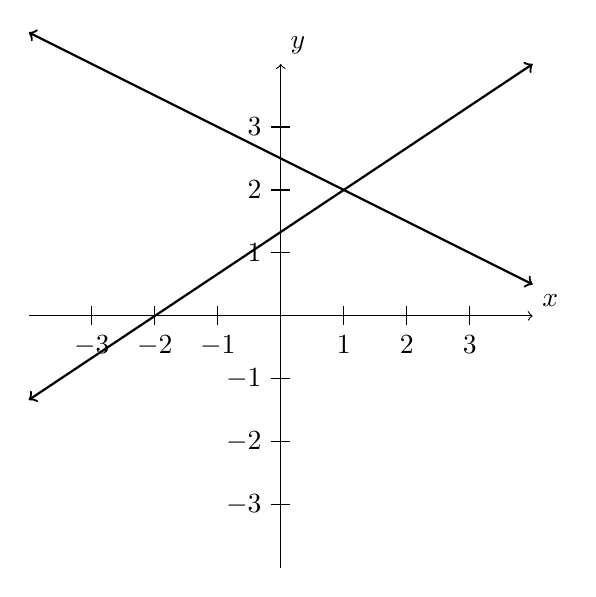
\begin{tikzpicture}[scale=0.8]
\draw[->] (-4,0) -- (4,0) node [above right] {$x$};
\draw[->] (0,-4) -- (0,4) node [above right] {$y$};
\foreach \x in {-3,-2,-1,1,2,3} {\draw (\x,0.15) -- (\x,-0.15) node [below] {$\x$};}
\foreach \y in {-3,-2,-1,1,2,3} {\draw (0.15,\y) -- (-0.15,\y) node [left] {$\y$};}

\draw[<->,thick] (-4,4.5) -- (4,0.5);
\draw[<->,thick] (-4,{(-4+8)/-3}) -- (4,{(-4-8)/-3});   
\end{tikzpicture}
\end{center}

The solution of the system is the point at which they cross.  In this case it looks like the point $(1,2)$ or $x=1$ and $y=2$.    This is an example where there is only one solution (or a \textbf{unique solution}).  \index{linear system!unique solution}

\item If we graph the lines in the linear system
%
\begin{align}
\begin{cases} \hspace{-0.1in}
\begin{split}
3x + 7 y  &= 10, \\
6 x + 14 y &=  5, 
\end{split}
\end{cases} \label{eq:linearsystem:geom2}
\end{align}
%
we get
\begin{center}
\begin{tikzpicture}[scale=0.8]
\draw[->] (-4,0) -- (4,0) node [above right] {$x$};
\draw[->] (0,-4) -- (0,4) node [above right] {$y$};
\foreach \x in {-3,-2,-1,1,2,3} {\draw (\x,0.15) -- (\x,-0.15) node [below] {$\x$};}
\foreach \y in {-3,-2,-1,1,2,3} {\draw (0.15,\y) -- (-0.15,\y) node [left] {$\y$};}

\draw[<->,thick] (-4,{(5+24)/14}) -- (4,{(5-24)/14});
\draw[<->,thick] (-4,{(10+12)/7}) -- (4,{(10-12)/7});   
\end{tikzpicture}
\end{center}
As you can see, it doesn't appear that the lines cross anywhere.  In fact, they don't because the lines are parallel.  This is an example of a linear system with \textbf{no solution}. 


\item The linear system
%
\begin{align}
\begin{cases}
x + 2 y  = 5, \\
2x + 4 y = 10,
\end{cases} \label{eq:linearsystem:geom3}
\end{align}
%
has the following graph for each line
\begin{center}
\begin{tikzpicture}[scale=0.8]
\draw[->] (-4,0) -- (4,0) node [above right] {$x$};
\draw[->] (0,-4) -- (0,4) node [above right] {$y$};
\foreach \x in {-3,-2,-1,1,2,3} {\draw (\x,0.15) -- (\x,-0.15) node [below] {$\x$};}
\foreach \y in {-3,-2,-1,1,2,3} {\draw (0.15,\y) -- (-0.15,\y) node [left] {$\y$};}

\draw[<->,thick] (-4,{(5+4)/2}) -- (4,{(5-4)/2});   
\end{tikzpicture}
\end{center}

It appears that there is only one line. This is because both lines have the same graph.  Each point on the line is a solution to the linear system and since there are an infinite number of such points, this is an example of a linear system with \textbf{infinite number of solutions}.  

\end{itemize}

You can see if you have two lines, each with two variables, the example in (\ref{eq:linearsystem:geom1}) is what happens if the two slopes are different.  In this case, there is one (or a \textbf{unique}) solution.\index{unique solution} \index{linear system!unique solution} 

In the other two cases as in equations (\ref{eq:linearsystem:geom2}) (\ref{eq:linearsystem:geom3}), both sets of lines have the same slope. In the case of (\ref{eq:linearsystem:geom2}) the lines have different $y$-intercepts, and therefore the lines are parallel and thus there is \textbf{no solution} to the linear system.  In the case of (\ref{eq:linearsystem:geom3}), both the slope and $y$-intercepts are equal, so the lines are equal and thus any point on the line is a solution, and this system has an \textbf{infinite number of solutions}.   


\subsection{Summaries of Linear Systems}

We will see more complicated linear systems (including systems with  more than two equations as well as more than two variables) shortly.  Even with more complicated systems, there are only three  possibilities for solutions linear systems:

\begin{itemize}
  \item One solution.  Mathematically, we say this is a \textbf{unique} solution. 
  \item No solution.  We often say that the system is \textbf{inconsistent}.\index{inconsistent linear system} \index{linear system!inconsistent}
  \item An infinite number of solutions.  We often say that such as system is \textbf{dependent}.  \index{dependent linear system} \index{linear system!dependent}
\end{itemize}

\subsection{Vectors in $\mathbb{R}^n$} 

Let's start simple and with something we know.  The notation $\mathbb{R}$ is the set of all real numbers.  It is often drawn as
%
\begin{center}
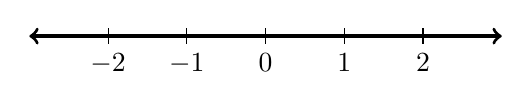
\begin{tikzpicture}
\draw[<->,very thick](-3,0) -- (3,0);

\foreach \x in {-2,-1,...,2} {\draw (\x,-0.1) -- (\x,0.1) node [at start, below] {$\x$};}
\end{tikzpicture}
\end{center}
and we use the number line to help with a number of mathematical concepts.  For example, $3 + 2$ means start at the point $3$ and go 2 spaces to the right (positive direction).  The point of this is that there is direction and magnitude on $\mathbb{R}$.  

\begin{definition}[Alternative Definition of a Vector]  
A \textbf{vector} is a mathematical object with a magnitude and a direction.  
\end{definition}

In $\mathbb{R}$, for two points, the vector between them is the distance between the point with the direction (left as negative and right as positive).  

In $\mathbb{R}^2$, vectors are often drawn as 
%
\begin{center}
\begin{tikzpicture}
\draw [->] (-4,0) -- (4,0); 
\draw [->] (0,-4) -- (0,4); 
\foreach \x in {-3,-2,-1,1,2,3} {\draw (\x,-0.1) -- (\x,0.1) node [at start, below] {$\x$};}
\foreach \y in {-3,-2,-1,1,2,3} {\draw (-0.1,\y) -- (0.1,\y) node [at start, left] {$\y$};}
\draw [->,very thick] (0,0) -- (3,2); 
\draw [->,very thick] (-3,-1) -- (0,1); 
\draw [->, very thick] (2,-1) -- (2,-2);  
\end{tikzpicture}
\end{center}
with the magnitude being the length of the arrow and the direction as the angle (typically from the positive horizontal axis).  

The left 2 vectors above are identical above because the have the same magnitude and direction.  That is the origin does not matter.  

To connect these concepts with that of vectors that we saw in section \ref{sect:matrices}  above, we saw that the two different vectors in the plot above are
%
\begin{align*}
\begin{bmatrix}
3 \\ 2
\end{bmatrix} &&& \begin{bmatrix}
0 \\ -1
\end{bmatrix}
\end{align*}
and as we will see that this formulation is much easier that writing down a vectors as a length and an angle.  

\subsubsection{Vectors, Free Vectors and Points}

As noted above, vectors by definition have only a direction and magnitude which is why two of the vectors in the figure above are equal.  Often, to clarify that the source point of the vector does not matter, the term \emph{free vector} is used.   However, generally, unless indicated a vector is a free vector.  

One case where a vector has a fixed point is when the source point is the origin.  For example:

\begin{center}
\begin{tikzpicture}
\draw [->] (-3,0) -- (3,0); 
\draw [->] (0,-3) -- (0,3); 
\foreach \x in {-2,-1,1,2} {\draw (\x,-0.1) -- (\x,0.1) node [at start, below] {$\x$};}
\foreach \y in {-2,-1,1,2} {\draw (-0.1,\y) -- (0.1,\y) node [at start, left] {$\y$};}
\draw [->,very thick] (0,0) -- (2,1) node [above] {$\vec{v}$}; 
\end{tikzpicture}
\end{center}

The vector starts at the origin and the end point is at the point $(2,1)$.  This vector is 
%
\begin{align*} \vec{v} & = 
\begin{bmatrix}
2 \\1
\end{bmatrix}
\end{align*}
and the vector and the end point are identical.  This can be very handy in many cases as we will we see.  



\subsubsection{Scalar Multiplication of Vectors}

In the previous chapter, we saw the scalar multiplication of a vector.  In $\mathbb{R}^2$, this means 
%
\begin{align*}
r \begin{bmatrix}
x_1 \\ x_2
\end{bmatrix} = \begin{bmatrix}
r x_1 \\ r x_2 
\end{bmatrix}
\end{align*}

 
in that each component of the vector is multiplied by the scalar $r$.  Geometrically, multiplication by the scalar $r$, \emph{scales} the length of the vector by a factor of $r$ and flips its direction if $r<0$.  

\begin{center}
\begin{tikzpicture}
\draw [->] (-3,0) -- (3,0); 
\draw [->] (0,-3) -- (0,3); 
\foreach \x in {-2,-1,1,2} {\draw (\x,-0.1) -- (\x,0.1) node [at start, below] {$\x$};}
\foreach \y in {-2,-1,1,2} {\draw (-0.1,\y) -- (0.1,\y) node [at start, left] {$\y$};}
\draw [->,very thick] (0,0) -- (2,1) node [above] {$\vec{v}$}; 
\draw [->,very thick] (0,-1) -- (4,1) node [right] {$2\vec{v}$};
\draw [->,very thick] (0,2) -- (-2,1) node [left] {$-\vec{v}$};    
\end{tikzpicture}
\end{center}

\subsubsection{Vector Addition}

As we saw in the previous chapter, vector addition in $\mathbb{R}^2$ is
%
\begin{align*}
\vec{u} + \vec{v} & = \begin{bmatrix}
u_1 \\ u_2 
\end{bmatrix} + \begin{bmatrix}
v_1 \\ v_2 
\end{bmatrix} = \begin{bmatrix}
u_1 + v_1 \\ u_2 + v_2 
\end{bmatrix}
\end{align*}
Consider two vectors $\vec{u}$ and $\vec{v}$ in the plane:

\begin{center}
\begin{tikzpicture}
\draw[->,very thick] (0,0) -- (2,1) node [midway, below right] {$\vec{u}$};  
\draw[->,very thick] (-2,1) -- (-1,4) node [midway, above left] {$\vec{v}$}; 
\end{tikzpicture}
\end{center}
The sum of these vectors can be represented by taking the $\vec{u}$ vector, then drawing the $\vec{v}$ at the tail end of the $\vec{u}$ vector.  The resulting vector 
\begin{center}
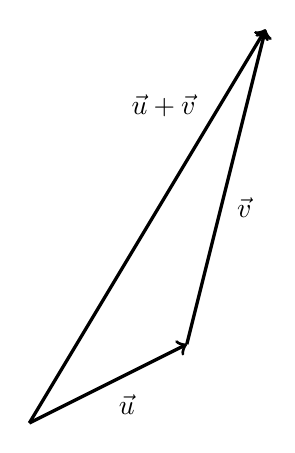
\begin{tikzpicture}
\draw[->,very thick] (0,0) -- (2,1) node [midway, below right] {$\vec{u}$}; 
\draw[->,very thick] (2,1) -- (3,5)node [midway, below right] {$\vec{v}$}; 

\draw[->,very thick] (0,0) -- (3,5) node [pos=0.75, above left] {$\vec{u}+\vec{v}$}; 
\end{tikzpicture}
\end{center}
starts at the beginning of $\vec{u}$ and ends at the end of $\vec{v}$ as seen above.  

Another way to think about this is to use $\vec{u}$ and $\vec{v}$ as the sides of the parallelogram.  The vector $\vec{u}+\vec{v}$ is diagonal from the starting point of both $\vec{u}$ and $\vec{v}$ extending to the ending point of both.  
\begin{center}
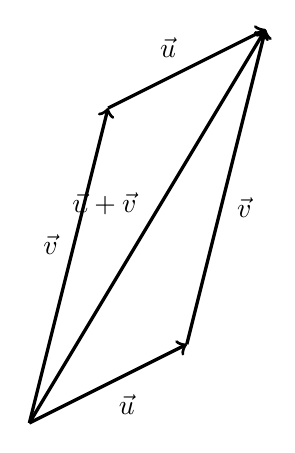
\begin{tikzpicture}
\draw[->,very thick] (0,0) -- (2,1) node [midway, below right] {$\vec{u}$}; 
\draw[->,very thick] (2,1) -- (3,5)node [midway, below right] {$\vec{v}$}; 
\draw[->,very thick] (1,4) -- (3,5) node [midway, above left] {$\vec{u}$};
\draw[->,very thick] (0,0) -- (1,4)node [midway, above left] {$\vec{v}$}; 

\draw[->,very thick] (0,0) -- (3,5) node [midway, above left] {$\vec{u}+\vec{v}$}; 
\end{tikzpicture}
\end{center}

\subsubsection{Geometry of Addition and Scalar Multiplication in $\mathbb{R}^n$}

As we saw in the previous section, we know how to add and scalar multiply vectors in $\mathbb{R}^n$.  The geometry of these operations are similar to that in $\mathbb{R}^2$.  For example, in $\mathbb{R}^3$, a vector connects two points in 3-dimensional space.  Scalar multiplication results in scaling that vector by a factor of $r$.  Addition works the same way: make the ending point of the first vector, the starting point of the second vector.  The result is the vector from the starting point of the first vector to the ending point of the 2nd vector.  

And this extends to any dimension, $\mathbb{R}^n$.  Although this is difficult to visualize, it still works the same way.  Typically there is no need to draw any vectors in dimensions above 3.  

\subsubsection{Lines in Vector form in $\mathbb{R}^2$ and $\mathbb{R}^3$}

First, let's look at a line in $\mathbb{R}^2$ and for example, passes through $(2,1)$ and $(3,4)$ and denote the line $L$. This would look like:
%
\begin{center}
\begin{tikzpicture}
\draw [->] (-4,0) -- (4,0); 
\draw [->] (0,-4) -- (0,4); 
\foreach \x in {-3,-2,-1,1,2,3} {\draw (\x,-0.1) -- (\x,0.1) node [at start, below] {$\x$};}
\foreach \y in {-3,-2,-1,1,2,3} {\draw (-0.1,\y) -- (0.1,\y) node [at start, left] {$\y$};}

\fill (2,1) circle (2.5pt);
\fill (3,4) circle (2.5pt);

\draw[<->] ({1/3},-4) -- ({10/3},5) node [pos=0.8,below right]{$L$}; 
\draw[->,very thick] (2,1) -- (3,4) node [at end, below right] {$\vec{v}$};  

\draw[->,very thick] (0,0) -- (2,1) node [midway, above] {$\vec{u}$};  

\draw[->,very thick, red] (2,1) -- (2.5,2.5) node [midway, below right] {$t\vec{v}$};  
\draw[->,very thick, red] (0,0) -- (2.5,2.5) node [pos=0.6, above left]  {$\vec{u}+t\vec{v}$};  
\end{tikzpicture}
\end{center}

Let's make the vector $\vec{v}$ the vector between the points $(2,1)$ and $(3,4)$ as shown on the figure above.  Recall that a vector and a point is synonymous if the vector starts at the origin.  Call $\vec{u}$ the vector from $(0,0)$ to $(2,1)$. 

Next, any point on the line can be written as a vector by addition of $\vec{u}$ and a scale of $\vec{v}$ or $\vec{u}+t\vec{v}$.  Thus the line between these two points can be written as
%
\begin{align*}
\{ 
\begin{bmatrix}
x \\ y 
\end{bmatrix} = 
\begin{bmatrix}
2 \\ 1
\end{bmatrix} + t 
\begin{bmatrix}
1 \\ 3
\end{bmatrix} \; | \; t \in \mathbb{R} \} 
\end{align*}

This notion extend easily to $\mathbb{R}^3$.  The set of points 
%
\begin{align*}
\{ 
\begin{bmatrix}
2 \\ 1 \\ 3
\end{bmatrix} + t \begin{bmatrix}
1 \\ 0 \\ 2
\end{bmatrix} \; | \; t \in \mathbb{R} \} 
\end{align*}


\tdplotsetmaincoords{70}{130}

\begin{center}
\begin{tikzpicture}[tdplot_main_coords]

%draw the main coordinate system axes
\draw[thick,->] (0,0,0) -- (4,0,0) node[anchor=north east]{$x$};
\draw[thick,->] (0,0,0) -- (0,4,0) node[anchor=north west]{$y$};
\draw[thick,->] (0,0,0) -- (0,0,4) node[anchor=south]{$z$};


\draw[-stealth] (0,0,0) -- (2,1,3) node [midway,above left] {$\vec{u}$};
\draw[-stealth,thick] (2,1,3) -- (4,1,1) node [midway,above left] {$t\vec{v}$}; 
\draw[<->] (0,1,5) -- (5,1,0); 


\end{tikzpicture}
\end{center}

\subsubsection{Planes in $\mathbb{R}^3$}  

A plane in $\mathbb{R}^3$ can also be written using vectors although perhaps harder to visualize.  

\begin{definition}
A \text{plane} in $\mathbb{R}^3$ is the set of points 
%
\begin{align*}
\{ \vec{p} + \vec{u} t + \vec{v} s \; | t,s \in \mathbb{R} \}
\end{align*}
for nonzero vectors $\vec{u}$ and $\vec{v}$ and $\vec{p},\vec{u}$ and $\vec{v}$ are vectors in $\mathbb{R}^3$.    
\end{definition}


Consider the following example in which a parallelogram is drawn in the plane.  The point $(2,3,1)$ in one corner of the parallelogram and the two sides are 
%
\begin{align*}
\vec{v} & = \begin{bmatrix}
1 \\ 1 \\1 
\end{bmatrix} & \vec{w} & = \begin{bmatrix}
2 \\ 0 \\ -1
\end{bmatrix}
\end{align*}

The parallelogram in $\mathbb{R}^3$ would look like:
%
\tdplotsetmaincoords{70}{130}

\begin{center}
\begin{tikzpicture}[tdplot_main_coords]

%draw the main coordinate system axes
\draw[thick,->] (0,0,0) -- (4,0,0) node[anchor=north east]{$x$};
\draw[thick,->] (0,0,0) -- (0,4,0) node[anchor=north west]{$y$};
\draw[thick,->] (0,0,0) -- (0,0,4) node[anchor=south]{$z$};


\draw[-stealth] (2,3,1) -- (1,1,1) node [midway,above right] {$\vec{v}$};
\draw[-stealth] (2,3,1) -- (4,3,0) node [midway,above left] {$\vec{w}$}; 

\draw[-stealth] (1,1,1) -- (3,1,0) -- (4,3,0); 




\end{tikzpicture}
\end{center}


The set of all points on the plane can then be written as 
%
\begin{align*}
\{ \begin{bmatrix}
2 \\ 3 \\ 1
\end{bmatrix} + \begin{bmatrix}
1 \\ 1 \\ 1
\end{bmatrix} t + 
\begin{bmatrix}
2 \\ 0 \\ -1
\end{bmatrix} s \; | \; t,s \in \mathbb{R} \}
\end{align*}

Extending this idea to linear surfaces in $\mathbb{R}^n$ is a natural generalization of planes.  
\begin{definition}
A \textbf{$k$-dimensional linear surface} in $\mathbb{R}^n$ is the set:
\begin{align*}
\{ \vec{p} + t_1 \vec{v}_1 + t_2 \vec{v}_2 + \cdots + t_k \vec{v}_k \; | \; t_1, t_2, \ldots, t_k \in \mathbb{R} \} 
\end{align*}
If $k=n-1$, then the surface is called a \textbf{hyperplane}.  
\end{definition}



\subsubsection{Geometry of Linear Systems}

You should have noticed the the $k$-dimensional linear surface above has the same form as the solution to the general linear system.  

\begin{itemize}
\item If the linear system has one free variable, the solution is a line. 
\item If the linear system has two free variables, the solution is a plane (or hyperplane).  
\end{itemize}


\subsection{Length and Angle Measures}  \label{sect:length:angles}

Two  of the basic ideas of geometry are the notions of length and angles.  These are well-defined in $\mathbb{R}^2$ and with a relatively easy extension to $\mathbb{R}^3$ and in this section we generalize to $\mathbb{R}^n$.   We'll start with the notion of distance as the length of a vector.  Consider first a vector
%
\begin{align*}
\vec{v} = \begin{bmatrix}
v_1 \\ v_2 
\end{bmatrix}
\end{align*}
in the plane ($\mathbb{R}^2$).   
\begin{center}
\begin{tikzpicture}
\draw [->] (-3,0) -- (3,0); 
\draw [->] (0,-3) -- (0,3); 
%\foreach \x in {-2,-1,1,2} {\draw (\x,-0.1) -- (\x,0.1) node [at start, below] {$\x$};}
%\foreach \y in {-2,-1,1,2} {\draw (-0.1,\y) -- (0.1,\y) node [at start, left] {$\y$};}
\draw [->,very thick] (0,0) -- (2,1) node [above] {$\vec{v}$}; 
\draw (2,0.1) -- (2,-0.1) node [below] {$v_1$};
\draw (0.1,1) -- (-0.1,1) node [left] {$v_2$};
\draw (2,0) -- (2,1) node [midway, right] {$v_2$}; 
%\draw [->,very thick] (0,-1) -- (4,1) node [right] {$2\vec{v}$};
%\draw [->,very thick] (0,2) -- (-2,1) node [left] {$-\vec{v}$};    
\end{tikzpicture}
\end{center}
and using plane geometry, the length of $\vec{v}$, denoted $||\vec{v}||$ is the hypotenuse of the triangle or
%
\begin{align*}
||\vec{v}|| & = \sqrt{v_1^2+v_2^2}
\end{align*}
and if $\vec{v}$ is in $\mathbb{R}^3$, the length would include a square of the third component inside the square root.  Thus, we defined the length of any vector in $\mathbb{R}^n$ to be the following. 

\begin{definition}
The \textbf{length} of a vector  $\vec{v} \in \mathbb{R}^n$ is given by 
%
\begin{align*}
|| \vec{v}|| & = \sqrt{v_1^2 + v_2^2 + \cdots v_n^2 } 
\end{align*}
which fits our expectations in $\mathbb{R}^2$ and $\mathbb{R}^3$.  
\end{definition}

\phantom{some text that doesn't show.}

~

\begin{example}
Find the length of the vector:
%
\begin{align*}
\vec{v}& = \begin{bmatrix}
3 \\ 1 \\ 0 \\ -5 
\end{bmatrix}
\end{align*}

\solution

\begin{align*}
||\vec{v}|| & = \sqrt{9+1+0+25} = \sqrt{35} 
\end{align*}
\end{example}

\subsubsection{Angles of vectors in $\mathbb{R}^2$} 

Consider first 2 vectors in $\mathbb{R}^2$.  The angle between them would be the angle (measured in the counterclockwise direction) between the vectors if the starting point is anchored at the same place.   For example:


\begin{center}
\begin{tikzpicture}[scale=0.8]
\draw [->] (-3,0) -- (4,0); 
\draw [->] (0,-3) -- (0,4); 
\foreach \x in {-2,-1,1,2,3} {\draw (\x,-0.1) -- (\x,0.1) node [at start, below] {$\x$};}
\foreach \y in {-2,-1,1,2,3} {\draw (-0.1,\y) -- (0.1,\y) node [at start, left] {$\y$};}


\draw[->] (0,0) -- (3,1) node [below right] {$\vec{u}$}; 
\draw[->] (0,0) -- (-1,2) node [below left] {$\vec{v}$}; 

\draw(9.48pt,3.16pt) arc [radius=10pt, start angle=18.43, end angle=116.56505118] ;

\draw(0.1,0.3) node [above right] {$\theta$}; 

\end{tikzpicture}
\end{center}
where 
%
\begin{align*}
\vec{u} & = \begin{bmatrix}
3 \\ 1
\end{bmatrix}, & \vec{v} & = \begin{bmatrix}
-1 \\ 2 
\end{bmatrix}
\end{align*}

You can find the angle using knowledge of geometry.  In this case, you can make a triangle by connecting the end points of each vector.  Note that the third leg of the triangle can be written as
%
\begin{align*}
\vec{v}-\vec{u} & = \begin{bmatrix}
-1 \\ 2
\end{bmatrix} - \begin{bmatrix}
3 \\ 1
\end{bmatrix} = \begin{bmatrix}
-4 \\ 1
\end{bmatrix}
\end{align*}


\begin{center}
\begin{tikzpicture}[scale=0.8]
\draw [->] (-3,0) -- (4,0); 
\draw [->] (0,-3) -- (0,4); 
\foreach \x in {-2,-1,1,2,3} {\draw (\x,-0.1) -- (\x,0.1) node [at start, below] {$\x$};}
\foreach \y in {-2,-1,1,2,3} {\draw (-0.1,\y) -- (0.1,\y) node [at start, left] {$\y$};}


\draw[->] (0,0) -- (3,1) node [midway, below right] {$\vec{u}$}; 
\draw[->] (0,0) -- (-1,2) node [midway, below left] {$\vec{v}$}; 
\draw[->] (3,1) -- (-1,2) node [midway, above] {$\vec{v}-\vec{u}$};  

\draw (9.48pt,3.16pt) arc [radius=10pt, start angle=18.43, end angle=116.56505118] ;

\draw(0.1,0.3) node [above right] {$\theta$}; 

\end{tikzpicture}
\end{center}
and the lengths of the three sides are:
%
\begin{align*}
||\vec{u}|| & = \sqrt{10}, & ||\vec{v}|| &= \sqrt{5}, & ||\vec{v}-\vec{u}|| & = \sqrt{17} 
\end{align*}
and then using the law of cosines:
%
\begin{align*}
||\vec{v}-\vec{u}||^2 & = ||\vec{u}||^2 + || \vec{v}||^2 -2 ||\vec{u}|| \,  ||\vec{v}| \cos \theta \\
17 & = 10+5 - 2 \sqrt{10}\sqrt{5} \cos \theta \\
\frac{2}{-2 \sqrt{10}\sqrt{5}} & = \cos \theta 
\end{align*}
which in this case $\theta \approx 98.13^{\circ}$.  


Note: since the range of $\cos^{-1} \theta$ is $[0,\pi]$ (or $[0,180^{\circ}]$), the angle will always be the angle between the vectors with this range.  If you need the proper angle, you may need to subtract the result from $360^{\circ}$.  


\subsubsection{Angles of vectors in $\mathbb{R}^n$}

\label{subsect:angles:vectors}

Understanding the above section allows us to extend the notion of vectors in $n$ dimensions, with the key being the law of cosines:
\begin{align*}
||\vec{u}-\vec{v}||^2 & = ||\vec{u}||^2 + || \vec{v}||^2 -2 ||\vec{u}|| \,  ||\vec{v}| \cos \theta \\
\end{align*}
and if we expand this out for 
%
\begin{align*}
\vec{u} & = \begin{bmatrix}
u_1 \\ u_2 \\ \vdots \\ u_n 
\end{bmatrix} & 
\vec{v} & = \begin{bmatrix}
v_1 \\ v_2 \\ \vdots \\ v_n 
\end{bmatrix} 
\end{align*}
Then 
%
\begin{align*}
||\vec{u}-\vec{v}||^2 & = (u_1-v_1)^2 + (u_2-v_2)^2 + \cdots + (u_n -v_n)^2, \\
||\vec{u}||^2 & = u_1^2 + u_2^2 + \cdots + u_n^2, \\
||\vec{v}||^2 & = v_1^2 + v_2^2 + \cdots + v_n^2, 
\end{align*}
Expanding the top equation and subtracting the two below:
%
\begin{align*}
||\vec{u}-\vec{v}||^2-||\vec{u}||^2-||\vec{v}||^2 & = -u_1v_1 - u_2v_2 - \cdots -u_nv_n 
\end{align*}
The negative of this expression appears often throughout linear algebra and is called the \textbf{dot product}

\begin{definition}
The \textbf{dot product} (or \textbf{inner product}) of the vectors $\vec{u}$ and $\vec{v}$ is defined as 
%
\begin{align*}
\vec{u} \cdot \vec{v} & = u_1v_1 + u_2v_2 + \cdots +u_nv_n 
\end{align*}
\end{definition}

Note:  the dot product between two vectors results in a number (a scalar).  Also, the dot product is only defined between two vectors of the same length.  Also, for any vector $\vec{u}$, there is a nice relationship between the length and the dot product:
%
\begin{align*}
\vec{u} \cdot \vec{u}  & = ||\vec{u}||^2
\end{align*}

Again, returning to law of cosines and solving for $\cos \theta$:
%
\begin{align*}
\cos \theta & = \frac{||\vec{u}-\vec{v}||^2-||\vec{u}||^2-||\vec{v}||^2}{-2 ||\vec{u}|| \, ||\vec{v}||} \\
& = \frac{-\vec{u} \cdot \vec{v}}{-2 ||\vec{u}|| \, ||\vec{v}||} \\ 
& = \frac{\vec{u} \cdot \vec{v}}{2 ||\vec{u}|| \, ||\vec{v}||} 
\end{align*}

\subsubsection{Properties of The Dot Product} \label{sect:dot:prod:props}

As we will see, the dot product is an extremely important concept.  Before going on, we show the properties of the dot product.  

\begin{description}
\item[(Commutative)]   $\vec{u} \cdot \vec{v} = \vec{v} \cdot \vec{u}$, 
\item[(Distributative)] $\vec{u} \cdot (\vec{v} + \vec{w}) = \vec{u} \cdot \vec{v} + \vec{u} \cdot \vec{w}$.  
\item[(Associative)] $\vec{u} \cdot (r\vec{v}) = (r \vec{u}) \cdot \vec{v}) = r (\vec{u} \cdot \vec{v})$.  
\end{description}

These properties can be shown using the Definition above.  



\begin{theorem}[The Triangle Inequality]
For any $\vec{u}$ and $\vec{v}$ both in $\mathbb{R}^n$, then 
%
\begin{align*}
||\vec{u}+\vec{v}|| &  \leq ||\vec{u}||+||\vec{v}|| 
\end{align*}

Equality is only reached if one of the vectors is a nonnegative scalar multiple of the other.  
\end{theorem}

This can be visualized by considering the plane in which $\vec{u}$ and $\vec{v}$ lie (and note that regardless of the value of $n$, they will lie in a plane or planar subset of $\mathbb{R}^n$.)


\begin{center}
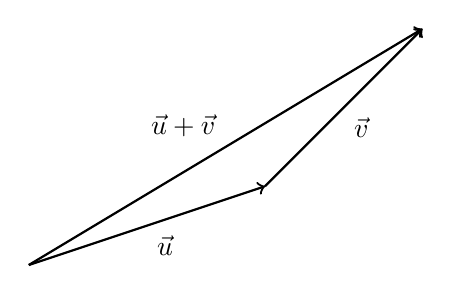
\begin{tikzpicture}
\draw[->, thick] (0,0) -- (3,1) node [midway,below right] {$\vec{u}$}; 
\draw[->,thick] (3,1) -- (5,3) node [midway,below right] {$\vec{v}$};
\draw[->,thick] (0,0) -- (5,3) node [midway,above left] {$\vec{u}+\vec{v}$}; 
\end{tikzpicture}
\end{center}

The vector $\vec{u}+\vec{v}$ is one side of the triangle and we know that any one side must always be no larger than the sum of the other two.  


\begin{proof}
We'll assume that the triangle inequality is true and show this results in another true statement. 
\begin{align}
||\vec{u}+\vec{v}||^2 & \leq (||\vec{u}|| + ||\vec{v}||)^2 \notag \\ 
(\vec{u}+\vec{v}) \cdot (\vec{u}+\vec{v}) & \leq ||\vec{u}||^2 + 2 ||\vec{u}|| \, ||\vec{v}|| + ||\vec{v}||^2 \notag \\ 
\vec{u}\cdot \vec{u} + 2 \vec{u} \cdot \vec{v} + \vec{v} \cdot \vec{v} & \leq \vec{u} \cdot \vec{u} + 2 || \vec{u}|| \, || \vec{v}|| + \vec{v} \cdot \vec{v}  \notag \\
2 \vec{u} \cdot \vec{v} & \leq 2 || \vec{u}|| \, || \vec{v}||  \label{eq:tri:inequal}
\intertext{multiply both sides by $||\vec{u}|| \, ||\vec{v}||$} 
2 (||\vec{v}|| \vec{u} ) \cdot (||\vec{u}|| \vec{v}) & \leq 2 ||\vec{u}||^2 || \vec{v}||^2  \notag \\
0 & \leq 2 ||\vec{u}||^2 || \vec{v}||^2 - 2 (||\vec{v}|| \vec{u} ) \cdot (||\vec{u}|| \vec{v}) \notag \\
0 & \leq ||\vec{u}||^2 \, ||\vec{v}||^2 - 2 (||\vec{v}|| \vec{u} ) \cdot (||\vec{u}|| \vec{v})  + || \vec{u} ||^2 \, || \vec{v}||^2  \notag \\
0 & \leq ||\vec{u}||^2 (\vec{v} \cdot \vec{v}) - 2 (||\vec{v}|| \vec{u} ) \cdot (||\vec{u}|| \vec{v}) + ||\vec{v}||^2 (\vec{u} \cdot \vec{u}) \notag \\
0 & \leq (||\vec{u}|| \vec{v}) \cdot (||\vec{u}|| \vec{v}) - 2 (||\vec{v}|| \vec{u} ) \cdot (||\vec{u}|| \vec{v}) + (||\vec{v}|| \vec{u}) \cdot (||\vec{u}|| \vec{v})   \notag \\
0 & \leq (||\vec{u}|| \vec{v}- ||\vec{v}|| \vec{u}) \cdot (||\vec{u}|| \vec{v} - ||\vec{v}||\vec{u}) \notag  \\
0 & \leq || ( ||\vec{u}|| \vec{v}- ||\vec{v}|| \vec{u}) ||^2 \notag
\end{align}
Since this statement is true and all steps are reversible, the triangle inequality is true. 

Now since the left hand side is a length, by definition it is greater than or equal to zero.  To show equality, assume that $||\vec{v}|| \neq 0$, 
%
\begin{align*}
||\vec{u}||\vec{v} - ||\vec{v}|| \vec{u} & = 0 \intertext{or}
\vec{u} & = \frac{||\vec{u}||}{||\vec{v}||} \vec{v}
\end{align*}
therefore $\vec{u}$ is a scalar multiple of $\vec{v}$.  
\end{proof}


\begin{corollary}[Cauchy-Swartz Inequality]
\begin{align*}
| \vec{u} \cdot \vec{v}| & \leq ||\vec{u}|| \, ||\vec{v}||
\end{align*}
with equality if and only if $\vec{u}$ and $\vec{v}$ are scalar multiples of each other. 
\end{corollary}


\begin{proof}
A consequence of the Triangle Inequality is (\ref{eq:tri:inequal}), thus the Cauchy-Swartz Inequality holds if $\vec{u} \cdot \vec{v} >0$.  Assume that $\vec{u} \cdot \vec{v} <0$.  Then 
%
\begin{align*}
\vec{u} \cdot \vec{v} = - (\vec{u} \cdot \vec{v}) = (-\vec{u} \cdot \vec{v}) & \leq ||-\vec{u}|| ||\vec{v}||   \intertext{and since $||-\vec{u}|| = ||\vec{u}||$}
& = ||\vec{u}|| \, ||\vec{v}|| 
\end{align*}

The equality condition is not shown. 
\end{proof}

We now use the dot product to define the angle between two vectors in $\mathbb{R}^n$.

\begin{definition}
The \textbf{angle between vectors $\vec{u}$ and $\vec{v}$} is the value of $\theta$ that satisfies:
\begin{align*}
\cos \theta & = \frac{ \vec{u} \cdot \vec{v}}{||\vec{u}||\, ||\vec{v}||}
\end{align*}

\end{definition}


So now with any two vectors, the above expression is a way to define the angle between them.  

\begin{example}
Find the angle between 
%
\begin{align*}
\vec{u} & = \begin{bmatrix}
2 \\ -4 \\ 1 \\ 1
\end{bmatrix} & \vec{v} & = \begin{bmatrix}
3 \\ 2 \\ 0 \\ 5 
\end{bmatrix}
\end{align*}

\solution

\begin{align*}
||\vec{u}|| & =\sqrt{22}, & ||\vec{v}|| & = \sqrt{38} \\
\end{align*}
\begin{align*}
\vec{u} \cdot \vec{v} & = 6-8+0+5 = 3 
\end{align*}
and therefore the angle can be found by 
%
\begin{align*}
\cos \theta & = \frac{3}{\sqrt{22}\sqrt{38}} \approx 0.1037571696
\end{align*}
and $\theta \approx 84.04^{\circ}$.   And although it's difficult to visualize these vectors, we can imagine the angle between them.  
\end{example}

One of the most important angles in geometry is $\theta=90^{\circ}$, which occurs in right triangles and perpendicular lines.  In terms of vectors, we use the dot product to define this.  

\begin{definition}
Two vectors $\vec{u}$ and $\vec{v}$ are \textbf{perpendicular} or \textbf{orthogonal} if their dot product is 0.  
\end{definition}



\vfill \pagebreak

\section{Reduced Row Echelon Form} \label{sect:reduced:row:echelon}

As we have seen in section \ref{sect:linear:syst}, there are numerous ways to reduce a matrix (or a linear system) to echelon form using Gauss's method.  For example:

%
\begin{align*}
\begin{bmatrix}
3 & 4 \\
1 & 2
\end{bmatrix}
\end{align*}

Can be reduced to any of the following:
%
\begin{align*}
\begin{bmatrix}
3 & 4 \\
0 & -2 
\end{bmatrix} &&
\begin{bmatrix}
1 & 2 \\
0 & -2 
\end{bmatrix} &&
\begin{bmatrix}
1 & 0 \\
0 & -2 
\end{bmatrix} 
\end{align*}

What row operations get us to these matrices?  

A question arises with this differences in the echelon forms of the matrices.  Are the solution sets equivalent?  The answer is yes.  Are the number, free variables the same?    The way we will answer this last question is by putting the matrix in \textbf{reduced row echelon form}.

\subsection{Gauss-Jordon Reduction}


We solved the linear system from Example \ref{ex:solve:linear:syst}.  
%
\begin{align*}
4x_1 - x_3 & = 0, \\
x_1+3x_2 +2x_3 & = 3, \\
3x_2 + 5x_3 & = 14. 
\end{align*}
%
by putting the array in echelon form using elementary row operations, 
\begin{align*}
\begin{bmatrix}[rrr|r]
4 & 0 & -1 & 0 \\
1 & 3 & 2 & 3 \\
0 & 3 & 5 & 14 
\end{bmatrix} \\
-R_1 + 4R_2 \rightarrow R_2,  \qquad
\begin{bmatrix}[rrr|r]
4 & 0 & -1 & 0 \\
0 & 12 & 9 & 12 \\
0 & 3 & 5 & 14 
\end{bmatrix} \\
-R_2 + 4R_3 \rightarrow R_3, \qquad
\begin{bmatrix}[rrr|r]
4 & 0 & -1 & 0 \\
0 & 12 & 9 & 12 \\
0 & 0 & 11 & 44 
\end{bmatrix} 
\end{align*}
then using back-substitution.  


Note that there is still work to be done to get the solution using back-sub\-sti\-tution.  Instead, we can continue to use Gauss' method to further reduce the matrix into a nicer form:

\begin{align*}
\frac{1}{11} R_3 \rightarrow R_3, & \qquad
\begin{bmatrix}[rrr|r]
4 & 0 & -1 & 0 \\
0 & 12 & 9 & 12 \\
0 & 0 & 1 & 4 \\
\end{bmatrix}  \\
\begin{array}{r}	
-9R_3+R_2 \rightarrow R_2, \\
R_3 + R_1 \rightarrow R_1, 
\end{array} & \qquad 
\begin{bmatrix}[rrr|r]
4 & 0 & 0 & 4 \\
0 & 12 & 0 & -24 \\
0 & 0 & 1 & 4 \\
\end{bmatrix}  \\
\begin{array}{r}
\frac{1}{12} R_2 \rightarrow R_2, \\[4pt]
\frac{1}{4} R_1 \rightarrow R_1, 
\end{array} & \qquad
\begin{bmatrix}[rrr|r]
1 & 0 & 0 & 1 \\
0 & 1 & 0 & -2 \\
0 & 0 & 1 & 4 \\
\end{bmatrix}  \\
\end{align*}

Now this is a nicer form, because if the linear system is written from the matrix, then:
%
\begin{align*}
x & = 1, \\
y & = -2, \\
z & = 4.
\end{align*}
or in vector form 
%
\begin{align*}
\vec{x} & = \begin{bmatrix}
1 \\ -2 \\ 4
\end{bmatrix}
\end{align*}
which is the last column of the matrix.  

\begin{definition}
A matrix is in \textbf{reduced row-echelon form}\index{reduced row-echelon form}\index{matrix!reduced row-echelon form} if in addition to being in echelon form, that each leading entry is a 1, and the leading entry is the only non-zero entry in the column.  
\end{definition}

\phantom{Empty Text}

\begin{example}
The following matrices are in reduced row echelon form.

\begin{align*}
\begin{bmatrix}
1 & 0 & 3 \\
0 & 1 & -2 
\end{bmatrix} &&
\begin{bmatrix}
1 & 2 & 0 & 0 & 5 \\
0 & 0 & 1 & 0 & -2 \\
0 & 0 & 0 & 1 & 3 \\
\end{bmatrix} &&
\begin{bmatrix}
1 & 0 & 3 & 2 \\
0 & 1 & 2 & 9 \\
0 & 0 & 0 & 0 
\end{bmatrix}
\end{align*}
\end{example}

\begin{example}
Explain why the following are not in reduced row echelon form:

\begin{align*}
\begin{bmatrix}
2 & 0 & 4 \\
0 & 1 & 3
\end{bmatrix} &&
\begin{bmatrix}
1 & 3 & 2 \\
0 & 1 & -1 
\end{bmatrix} &&
\begin{bmatrix}
0 & 1 & 3 & 3 \\
1 & 0 & 2 & -1 
\end{bmatrix}
\end{align*}

\solution

\begin{itemize}
\item The first matrix is not in row reduced echelon form because the leading term in row 1 needs to be a 1, not a 2. 
\item The second matrix is not in row reduced echelon form because the column with the leading term in row 2 (which is column 2) should be 0 except the 1 in the second row. 
\item The third matrix is not in row reduced echelon form because the matrix is not in echelon form. 
\end{itemize}
\end{example}

\begin{definition}
The reduction of a matrix to reduced row echelon form using the three standard row operations is called \emph{Gauss-Jordon reduction} or the \emph{Gauss-Jordon method}.  
\end{definition}



As seen above, reduced row echelon form makes linear systems with a unique solution very easy to write down---the solution is in the last row.  We will also see that this form makes solutions with many solutions easier to write down as well.  

\begin{example}
Put the following linear system:
\begin{align*}
x_1\phantom{+2x_3} + 3x_3 -9 x_4 + 11 x_5 & = 14, \\
2x_3 \phantom{-9x_4} +\phantom{1} 4x_5 & = 10, \\
3x_5 & = 27, 
\end{align*}
into reduced row echelon form. 

\solution

First, this is already in echelon form, so we only need to do the steps to get to reduced row echelon form:
\begin{align*}
& \qquad 
\begin{bmatrix}[rrrrr|r]
1 & 0 & 3 & -9 & 11 & 14 \\
0 & 0 & 2 & 0 & 4 & 9 \\
0 & 0 & 0 & 0 & 3 & 27 
\end{bmatrix} \\
\frac{1}{3} R_3 \rightarrow R_3, & \qquad 
\begin{bmatrix}[rrrrr|r]
1 & 0 & 3 & -9 & 11 & 14 \\
0 & 0 & 2 & 0 & 4 & 9 \\
0 & 0 & 0 & 0 & 1 & 9 
\end{bmatrix} \\
\begin{array}{r}
-4 R_3 + R_2 \rightarrow R_2, \\
-11R_3 + R_1 \rightarrow R_1, 
\end{array} & \qquad
\begin{bmatrix}[rrrrr|r]
1 & 0 & 3 & -9 & 0 & -85 \\
0 & 0 & 2 & 0 & 0 & -26 \\
0 & 0 & 0 & 0 & 1 & 9 
\end{bmatrix} \\
\frac{1}{2} R_2 \rightarrow R_2, & \qquad
\begin{bmatrix}[rrrrr|r]
1 & 0 & 3 & -9 & 0 & -85 \\
0 & 0 & 1 & 0 & 0 & -13 \\
0 & 0 & 0 & 0 & 1 & 9 
\end{bmatrix} \\
-3R_2 + R_1 \rightarrow R_1, & \qquad
\begin{bmatrix}[rrrrr|r]
1 & 0 & 0 & -9 & 0 & -46 \\
0 & 0 & 1 & 0 & 0 & -13 \\
0 & 0 & 0 & 0 & 1 & 9 
\end{bmatrix}
\end{align*}
And now this is in reduced row echelon form.  The linear system from this equation can be written by solving for the leading variables:
%
\begin{align*}
x_1 & = -46 + 9x_4, \\
x_3 & = -13 \\
x_5 & = 9 
\end{align*}
and then the solution can be written in vector for as 
%
\begin{align*}
\{ \begin{bmatrix}
-46 \\
0 \\
-13 \\
0 \\
9
\end{bmatrix} + 
\begin{bmatrix}
0 \\ 1 \\ 0 \\ 0 \\ 0 
\end{bmatrix} x_2 + \begin{bmatrix}
9 \\ 0 \\ 0 \\ 1 \\ 0
\end{bmatrix} x_4 \; | \; x_2, x_4 \in \mathbb{R}, \} 
\end{align*}
which is the same solution as that from that in Example \ref{ex:large:linear:solution}.  

An alternative way to read off the solution from the reduced row echelon matrix is to add rows of zeros where the free variables would be.  In this case in row 1 and 4 and pushing others down. 

\begin{align*}
\begin{bmatrix}[rrrrr|r]
0 & 0 & 0 & 0 & 0 & 0 \\
0 & 1 & 0 & -9 & 0 & -\frac{89}{2} \\
0 & 0 & 1 & 0 & 0 & -\frac{27}{2} \\
0 & 0 & 0 & 0 & 0 & 0 \\
0 & 0 & 0 & 0 & 1 & 9 \\
\end{bmatrix}
\end{align*}
The particular solution is now the last column.  The solution also contains $x_1$ terms which is the first column with a 1 instead of a 0 in the first row and also the fourth column with a 1 instead of a 0 in the fourth row times $x_4$.  

\end{example}

~

\phantom{Empty sTff}


\begin{example}
Write down the solution set of the following linear system given in the reduced row echelon form of the matrix:
%
\begin{align*}
\begin{bmatrix}[rrrrrr|r]
1 & 0 & 3 & 0 & 0 & 5  & 11 \\
0 & 1 & -4 & 0 & 0 & 9 & -4 \\
0 & 0 & 0 & 1 & 0 & 3  & 5 \\
0 & 0 & 0 & 0 & 1 & 0 & -2 \\
\end{bmatrix}
\end{align*}
If we add a row between the 2nd and 3rd rows as well as after the fourth row, the matrix is:
%
\begin{align*}
\begin{bmatrix}[rrrrrr|r]
1 & 0 & 3 & 0 & 0 & 5  & 11 \\
0 & 1 & -4 & 0 & 0 & 9 & -4 \\
0 & 0 & 0 & 0 & 0 & 0 & 0 \\
0 & 0 & 0 & 1 & 0 & 3  & 5 \\
0 & 0 & 0 & 0 & 1 & 0 & -2 \\
0 & 0 & 0 & 0 & 0 & 0 & 0 
\end{bmatrix}
\end{align*}
The the solution set is 
%
\begin{align*}
\{ \begin{bmatrix}
11 \\ -4 \\ 0 \\ 5 \\ -2 \\ 0 
\end{bmatrix} + \begin{bmatrix}
-3 \\ 4 \\ 1 \\ 0 \\ 0 \\ 0 
\end{bmatrix} x_3 + 
\begin{bmatrix}
-5 \\ -9 \\ 0 \\ -3 \\ 0 \\ 1
\end{bmatrix} x_6 \; | \; x_3, x_6 \in \mathbb{R} \} 
\end{align*}
Recalling that you need to replace the 0 in the 3rd row of the $x_3$ vector with a 1  and replace the 0 in the 6th row of the $x_6$ vector with a 1.  
\end{example}

\subsubsection{Matrix Reduction is Matrix Equivalence} 

We have used the term \emph{matrix reduction} in converting a matrix to either echelon or reduced row echelon form.  

\begin{definition}
Two matrices that are interreducible by the elementary row operations are \textbf{row equivalent}.
\end{definition}


\subsection{Row Equivalence}

\begin{lemma}
A linear combination of linear combinations is a linear combination.
\end{lemma}

\begin{proof}
Consider the $m$  linear combinations $c_{1,1} x_1 + \cdots + c_{1,n} x_n$ through $c_{m,1} x_1 + \cdots + c_{m,n} x_n$.  A linear combination of these is
%
\begin{align*}
& d_1 (c_{1,1} x_1 + \cdots + c_{1,n} x_n ) + \cdots + d_m (c_{m,1} x_1 + \cdots + c_{m,n} x_n) \\
& \qquad = d_1 c_{1,1} x_1 + \cdots + d_1 c_{1,n} x_n + \cdots + d_m c_{m,1} x_1 + \cdots + d_m c_{m,n} x_n \\
& \qquad = (d_1 c_{1,1} + \cdots + d_m c_{m,1}) x_1 + \cdots + (d_1 c_{1,n} + \cdots + d_m c_{m,n}) x_n 
\end{align*}
\end{proof}

We will use the same convention as in the text.  That is for a matrix named with a capital roman letter, the $i$th row will be denoted with the equivalent lower-case greek with subscript $i$, that is
%
\begin{align*}
A & = \begin{bmatrix}
\cdots & \alpha_1 & \cdots \\
\cdots & \alpha_2 & \cdots \\
& \vdots & \\
\cdots & \alpha_n & \cdots \\
\end{bmatrix} & 
B & = \begin{bmatrix}
\cdots & \beta_1 & \cdots \\
\cdots & \beta_2 & \cdots \\
& \vdots & \\
\cdots & \beta_n & \cdots \\
\end{bmatrix} 
\end{align*}

\begin{corollary} \label{cor:rows:linear:comb}
When one matrix is transformed to another matrix, each row of the second is a linear combination of the first. 
\end{corollary}

\begin{proof}	
The base step, we prove that zero row operations that transforms $A$ to $B$, satisfies the corollary. In this case, 
%
\begin{align*}
\vec{\beta}_i & = 0 \cdot \alpha_1+ 0 \alpha_2 + \cdots + 1 \cdot \alpha_i + \cdots + 0 \cdot \alpha_n \qquad \text{for each $i=1, 2, \ldots, n$}.  
\end{align*}
so each row of $B$ is a linear combination of $A$. 

For the inductive step, assume that transforming $A$ to $B$ in $t+1$ steps.  Also assume that the matrix in the step before $B$ is called $G$, or
%
\begin{align*}
A \rightarrow \cdots \rightarrow G \rightarrow B
\end{align*}
with each arrow denoting a row operation.  Now we proceed showing that each of the 3 elementary row operations are linear combinations.   If $G \rightarrow B$ is given by 

\begin{enumerate}[label=(\roman*)]
\item $c R_i \rightarrow R_i$, then 
%
\begin{align*}
\vec{\beta}_j & = \begin{cases}
c \vec{\gamma}_j & \text{if $i=j$} \\
\vec{\gamma}_j & \text{otherwise} 
\end{cases}
\end{align*}
each of which is a linear combination of the rows of $G$, 
\item $R_i \leftrightarrow R_j$, for $i \neq j$, then 
%
\begin{align*}
\vec{\beta}_k  & = \begin{cases}
\vec{\gamma}_i & \text{if $k=j$} \\
\vec{\gamma}_j & \text{if $k=i$} \\ 
\vec{\gamma}_k & \text{otherwise}
\end{cases}
\end{align*}
again, each of which is a linear combination of the rows of $G$. 

\item $c R_i + R_j \rightarrow R_j$ for $i \neq j$, then 
\begin{align*}
\vec{\beta}_k  & = \begin{cases}
c \vec{\gamma}_k+ \vec{\gamma}_j & \text{if $k=i$} \\ 
\vec{\gamma}_k & \text{otherwise}
\end{cases}
\end{align*}
again, each of which is a linear combination of the rows of $G$. 
 

\end{enumerate}

Now this proves that for the step $G \rightarrow B$, each row of $B$ is a linear combination of rows of $G$.  

Now, using induction, since the first $t$ steps transforming $A$ to $G$ is a linear combination, the steps from $A$ to $B$, each row of $B$ is a linear combination of rows of $A$ because linear combinations of linear combinations are linear combinations.  

\end{proof}

\vfill \pagebreak

\begin{example}
Show that the steps that transform:
%
\begin{align*}
&\begin{bmatrix}
0 & 3 \\
1 & 2 
\end{bmatrix} \\
  R_1 \leftrightarrow R_2  \qquad &
\begin{bmatrix}
1 & 2 \\
0 & 3 \\
\end{bmatrix} \\ 
\frac{1}{3} R_2 \rightarrow R_2 \qquad & 
\begin{bmatrix}
1 & 2 \\
0 & 1 \\
\end{bmatrix} \\
 -2 R_2 + R_1 \rightarrow R_1 \qquad  &
\begin{bmatrix}
1 & 0 \\
0 & 1 
\end{bmatrix}
\end{align*}
are each linear combinations of row operations. 

\solution

Call the 4 matrices, $A$, $D$, $G$ and $B$, then 
%
\begin{align*}
\begin{split}
\delta_1 & = \alpha_2 \\
\delta_2 & = \alpha_1 
\end{split} &&&
\begin{split}
\gamma_1 & = \alpha_1 \\
\gamma_2 & = \frac{1}{3} \alpha_2 \\
\end{split} &&&
\begin{split}
\beta_1 & = -2 \gamma_2 + \gamma_1 \\
\beta_2 & = \gamma_2 
\end{split}
\end{align*}
\end{example}

\subsubsection{Echelon Form and Linear Combinations of Rows}

Let's return to echelon form.  Why is this a nice form?  Well we can use back substitution to solve for the leading variables.  The reason this works is the following lemma

\begin{lemma}In an echelon form matrix, no nonzero row is a linear combination of the other rows.   \label{lem:ech:ind}
\end{lemma}


In lieu of a proof, let's take a look at an example.  Consider  the echelon form matrix of a the linear system from Example \ref{ex:large:linear:solution}:
%
\begin{align*}
\begin{bmatrix}[rrrrr|r]
0 & 1 & 3 & -9 & 11 & 14 \\
0 & 0 & 2 & 0 & 4 & 9 \\
0 & 0 & 0 & 0 & 3 & 27 \\
\end{bmatrix}
\end{align*}

We look and determine if the second row (as an example) is a linear combination of the other two rows.  Thus:
%
\begin{align*}
\begin{bmatrix}
0 & 0 & 2 & 0 & 4 & 9 \\
\end{bmatrix} & = c_1 \begin{bmatrix}
0 & 1 & 3 & -9 & 11 & 14 
\end{bmatrix} + c_2 \begin{bmatrix}
0 & 0 & 0 & 0 & 3 & 27 
\end{bmatrix}
\end{align*}

Each component then becomes an equation for the linear system:
%
\begin{align*}
0 c_1 + 0 c_2 & = 0 \\
c_1 + 0 c_2 & = 0 \\
3 c_1 + 0 c_2 & = 2 \\
-9 c_1 + 0 c_2 & = 0 \\
11 c_1 + 3 c_2 & = 4 \\
14 c_1 + 27 c_2 & = 9 
\end{align*}
which can be written as the augmented matrix:
%
\begin{align*}
\begin{bmatrix}[rr|r]
0 & 0 & 0 \\
1 & 0 & 0 \\
3 & 0 & 2 \\
-9 & 0 & 0 \\
11 & 3 & 4 \\
14 & 27 & 9\\
\end{bmatrix} 
\end{align*}
if we transform this to row echelon form we get:
%
\begin{align*}
\begin{bmatrix}[rr|r]
14 & 27 & 9\\
0 & -3 & -1\\
0 & 0 & 28\\
0 & 0 & 0\\
0 & 0 & 0\\
0 & 0 & 0\\
\end{bmatrix}
\end{align*}
and the 3rd row says ``no solution'', so that the 2nd row is not a linear combination of the other two rows.  One can show this is also true for the other two rows.  

The notation of rows not being linear combinations of other rows is called \textbf{independence} and will be defined more-explicitly later in the course, however this example should give you a sense of what independence means.  

%\begin{proof}
%(of Lemma \ref{lem:ech:ind}) 
%
%\bigskip
%
%This will be a proof by contradiction.  Assume that the $i$th row is a linear combination of the other rows of the matrix that is it can be written:
%%
%\begin{align}
%\alpha_i & = c_1 \alpha_1 + c_2 \alpha_2 + \cdots + c_{i-1} \alpha_{i-1} + c_{i+1} \alpha_{i+1} + \cdots + c_m \alpha_m 
%\label{eq:row:linear:comb}
%\end{align}
%The matrix $A$ can be written as
%\begin{align*}
%A & = 
%\begin{bmatrix}
%0 & \cdots & 0 & \alpha_{1,\ell_1} & \alpha_{1, \ell_1+1} & \cdots & \alpha_{1,\ell_i} & \cdots & \alpha_{1,\ell_m} \\
%0 & \cdots & 0 & 0 & \alpha_{2,\ell_2} & \cdots & \alpha_{2,\ell_i} & \cdots & \alpha_{2, \ell_m} \\
%& & & & & & \vdots & & & \vdots \\ 
%\vdots &  & \vdots & & 0 & & \alpha_{i,\ell_i}   & & \vdots \\
%0 & \cdots & 0 & 0 & 0 & 0 & 0 & \\
%0 & \cdots & & & & &0  &0  & \alpha_{m,\ell_m} 
%\end{bmatrix}
%\end{align*}
%
%To find the values of $c_j$ in (\ref{eq:row:linear:comb}), evaluate that equation for any column.  To begin, consider $\ell_1$, the column of the leading coefficient of the first row.  Because the matrix is in echelon form, $\alpha_{2,\ell_1}, \alpha_{3,\ell_1}, \ldots, \alpha_{m,\ell_1}$ are all zero.  Thus, examining the $\ell_1$th element of (\ref{eq:row:linear:comb}), one gets:
%%
%\begin{align*}
%0 & = c_1 \alpha_{1,\ell_1} + c_2 \cdot 0 + \cdots + c_m \cdot 0
%\end{align*}
%and because $\alpha_{1,\ell_1} \neq 0$ (it is a leading element),  $c_1=0$.  
%
%Inductively, assume that $c_1,c_2, \ldots, c_{k-1}=0$,    (exercise?) 
%
%Let $\ell_k$ be the column with the leading element in row $k$.  This means that
%$\alpha_{k+1,\ell_k}, \alpha_{k+2,\ell_k}, \ldots, \alpha_{m,\ell_k}$ are all zero.  If we examine the $\ell_k$th component of (\ref{eq:row:linear:comb}), then 
%
%
%Let $\ell_i$ be the column with the leading element in row $i$.  If the $\ell_i$th element of (\ref{eq:row:linear:comb}) is extracted, one gets 
%%
%\begin{align*}
%\alpha_{i,\ell_k} & = (0) \alpha_{1,\ell_k} + (0) \alpha_{2,\ell_k} + \cdots + (0) \alpha_{i-1,\ell_k} + (0)  \alpha_{i+1,\ell_k} \\
%& \qquad + \cdots +  c_k\alpha_{k,\ell_k} + c_{k+1} \cdot 0 + \cdots + c_m \cdot 0 
%\end{align*}
%
%If $i>k$, then $\alpha_{i,\ell_k}=0$, and this implied that $c_k=0$.  If $i<k$, then 
%
%{\color{red}  Help, too hot to think.}  
%
%
%
%
%
%
%\end{proof}
%
%
%\begin{lemma}
%If two echelon form matrices are row equivalent then the leading entries in their first rows lie in the same column. The same is true of all the nonzero rows---the leading entries in their second rows lie in the same column, etc.
%\end{lemma}
%
%
%



\vfill \pagebreak

\section{Matrix Operations}
\label{sect:matrix:operations}

As we have seen, a matrix is a group of numbers arranged in a rectangular block.  An $m$ by $n$ matrix has $m$ rows and $n$ columns. 

For example,
%
\begin{align}
\begin{bmatrix}[rrrr]
1 & 2 & 11 & -1 \\ 3 & -2 & 3 & 4
\end{bmatrix}, \label{eq:example:matrix}
\end{align}
is a 2 by 4 matrix.

The \textbf{size}\index{matrix!size} of a matrix is the number of rows and columns in the matrix.  The number of rows is listed first.  The size of the example above is 2 by 4.  

The numbers in a matrix are called the \textbf{entries} or \textbf{elements} of the matrix.  For example, for the matrix in (\ref{eq:example:matrix}), the entry on the first row and third column is 11.  Often we will use the notation $a_{1,3} = 11$, where the subscript 1 is the row number and $3$ is the column number. 

\subsection{Matrix, Vector and Scalar Notation}

A \textbf{scalar} is a fancy term for a number.  Mathematician use this term to distinguish them from matrices and vectors, which are not scalars.  Whenever variables are used for scalars, then lower case letters will be used.  For example, $a, n$ and $x$ are scalar variables.  

When we use variable names for matrices, we will use capital letters.  For example, $A, B$ and $X$ are matrix (or vector) variables.  

\subsection{Addition and Subtraction of Matrices}


In this section, we learn how to perform some basic operations between matrices.  First, we will look at adding and subtracting two matrices and later we will look at multiplying a matrix by a scalar (a number).  

\begin{definition}
In this case, let $k \in \mathbb{R}$ and $A$ and $B$ are $m \times n$ matrices.  Then 

\begin{itemize}
\item $kA$ is the matrix formed by each entry is $ka_{i,j}$.  That is multiply each entry by $k$. 
\item $A+B$ is the matrix form by each entry is $a_{i,j}+b_{i,j}$.  That is to add matrices, we add element by element. 
\item $A-B$ is the matrix form by each entry is $a_{i,j}-b_{i,j}$.  That is to add matrices, we subtract element by element. 
\end{itemize}
If $A$ and $B$ are not the same size then $A+B$ and $A-B$ does not exist.  
\end{definition}

Note: an alternative definition of matrix subtraction, $A-B=A+(-B)$, which is consistent with subtraction of real numbers.  

\bigskip 
\begin{example}
Let
%
\begin{align*}
A & = \begin{bmatrix}
1 & -1 & 3 \\
2 & 7 & 3
\end{bmatrix} & 
B & = \begin{bmatrix}
3 & 2 & -7 \\ 11 & 2 & 0
\end{bmatrix}
\end{align*}

Then the sum $A+B$ is found by adding the individual elements. 
%
\begin{align*}
A+B & = \begin{bmatrix}
1+3 & -2+2 & 3-7\\ 2+11 & 7+2 & 3+0
\end{bmatrix}= \begin{bmatrix}
4 & 1 & -4 \\ 13 & 9 & 3
\end{bmatrix}
\end{align*}
similarly we can subtract in the same way
\begin{align*}
A-B & = 
\begin{bmatrix}
1-3 & -1-2 & 3-(-7)\\ 
2-11 & 7-2 & 3-0 
\end{bmatrix}= 
\begin{bmatrix}
-2 & -3 & 10 \\ 
-9 & 5 & 3 
\end{bmatrix}
\end{align*}

\end{example}


\begin{example}
 Find the following result or state that it does not exist. 
 % 
\begin{align*}
\begin{bmatrix}
 1 & 0 \\ 3 & -2 
\end{bmatrix} + 
\begin{bmatrix}
 3 & -2 \\
 5 & 0 \\
 -3 & 4
\end{bmatrix}
\end{align*}

\solution

Since the matrices are not the same size, this operation is not valid.  

\end{example}

\subsubsection{Scalar Multiplication of Vectors and Matrices}

Scalar multiplication of vectors and matrices is a simple operation where the result is the scalar times each element of the vector or matrix.  

\begin{example}
	Evaluate
	
	
\begin{enumerate}[label=(\alph*)]
\item 
\begin{align*} 3
\begin{bmatrix}
	5 & 5 \\
-4 & 2
\end{bmatrix}.
\end{align*} 

\item \begin{align*}
-7 \begin{bmatrix}
 3 & -2 & 0 & 5 
\end{bmatrix}
\end{align*}
\end{enumerate}

\solution

\begin{enumerate}[label=(\alph*)]
\item 
\begin{align*}
\begin{bmatrix}
	15 & 15 \\ -12 & 6
\end{bmatrix}
\end{align*}

\item 
\begin{align*}
\begin{bmatrix}
 -21 & 14 & 0 & -35 
\end{bmatrix}
\end{align*}
\end{enumerate}
\end{example}

\subsection{Transpose} \label{sect:transpose}

The last basic matrix operation that we will cover here in the transpose of a matrix.  As an example, if
%
\begin{align*}
	A & = 
\begin{bmatrix}
	3 & -1 & 0 \\ 2 & 7 & 5
\end{bmatrix}
\end{align*}
then the transpose is the matrix, $A^{\intercal}$ given by
% 
\begin{align*}
	A^{\intercal} & = 
\begin{bmatrix}
	3 & 2 \\ -1 & 7 \\ 0 & 5
\end{bmatrix}
\end{align*}
where the row and column of each element is flipped.  

\begin{definition}
The \textbf{transpose} of an $m \times n$ matrix $A$,  denoted $A^{\intercal}$ is $A$ flipped over the diagonal.  In particular, the element in the $i$th row and $j$th column of $A^{\intercal}$ is given by the $j$th row and $i$ column of $A$.  
\end{definition}

\subsubsection{Properties of Transposes}

We will see that transposes play a big role in linear algebra.  

\begin{lemma}
The following are true:
\begin{enumerate}
\item $(A+B)^{\intercal} = A^{\intercal} + B^{\intercal}$
\item $(cA)^{\intercal} = c A^{\intercal}$
\item $(A^{\intercal})^{\intercal} = A$.
\item $(AB)^{\intercal} = B^{\intercal} A^{\intercal}$ 
\end{enumerate}
\end{lemma}

%
\subsection{Multiplication of Vectors and Matrices}
\label{sect:mult:matrix}

In an perhaps backwards way of thinking, we will start with the product of two matrices.  We will then see that the product of matrices and vectors and then vectors and vectors can be seen in the same manner.  

\begin{definition}
Let $A$ and $B$ be matrices.  The \text{product of $A$ and $B$}, or $C=AB$ can be found in the following manner.  Element $c_{ij}$ is the dot product of the $i$th row of $A$ and the $j$th column of $B$.   

Note:  In order for the dot product to be defined, the number columns of $A$ must equal the number of rows of $B$.  If not the product is not defined.   
\end{definition}

Also if the product $AB$ is defined, the result, $C$ has the same number of rows of $A$ and the same number of columns as $B$.  

\begin{example}
Find $C=AB$ if
%
\begin{align*}
A & = \begin{bmatrix}
2 & -1 & 3 \\ 1 & 1 & 2 
\end{bmatrix}
&
B & = \begin{bmatrix}
2 & 1 \\ 3 & -2 \\ 7 & 5
\end{bmatrix}
\end{align*}

\solution

First, since the number of rows of $A$ is 2 and the number of columns of $B$ is 2, the size of $C$ is 2. 

\begin{itemize}
\item The 1st row and 1st column of $C$ is the 1st row of $A$ times the 1st column of $B$.   
\item The 1st row and 2nd column of $C$ is the 1st row of $A$ times the 2nd column of $B$.   
\item The 2nd row and 1st column of $C$ is the 2nd row of $A$ times the 1st column of $B$.   
\item The 2nd row and 2nd column of $C$ is the 2nd row of $A$ times the 2nd column of $B$.   

\end{itemize}

We now explicitly show the dot products.  

\begin{align*}
C & =
\begin{bmatrix}
\begin{bmatrix}
 2  & -1 & 3 	
\end{bmatrix}
\begin{bmatrix}
2 \\ 3 \\ 7
\end{bmatrix}
& 
\begin{bmatrix}
2 & -1 & 3 
\end{bmatrix}
\begin{bmatrix}
1 \\ -2 \\ 5
\end{bmatrix} \\
\begin{bmatrix}
1 & 1 & 2
\end{bmatrix}
\begin{bmatrix}
2 \\ 3 \\ 7
\end{bmatrix}
& 
\begin{bmatrix}
1 & 1 & 2
\end{bmatrix}
\begin{bmatrix}
1 \\ -2 \\ 5
\end{bmatrix}
\end{bmatrix}
 \\
& = 
\begin{bmatrix}
2(2) + (-1)(3) + 3(7) & (2)(1) + (-1)(-2) + (3)(5) \\
(1)(2) + (1)(3) +(2)(7) & (1)(1) + (1)(-2) + (2)(5) 
\end{bmatrix} \\
& = \begin{bmatrix}
22 & 19 \\ 19 & 9 
\end{bmatrix}
\end{align*}

\end{example}

\subsection{Size Restrictions on Matrices}

Note that for each element in the resulting matrix, there is a vector-vector product, coming from each row of the first matrix and each column of the second matrix: 

\begin{Boxed*}
The number of columns of the first matrix must equal the number of rows of the second matrix.
\end{Boxed*}

The size of the resulting matrix can also be found by the sizes of the input matrices.  

\begin{Boxed*}
If the matrices $A$ and $B$ are multiplied then this diagram helps with a valid product as well as the size of the result. 

\begin{center}
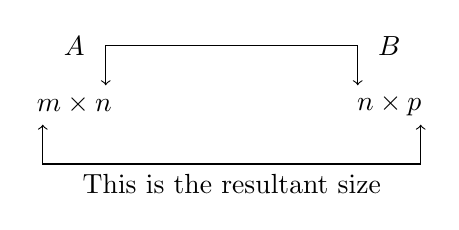
\begin{tikzpicture}
\draw (-2,-0.25) node[above] {$A$};
\draw (2,-0.25) node [above] {$B$};

\draw (-2,-0.75) node {$m \times n$};
\draw (2,-0.75) node {$n \times p$};

\draw[<->] (-1.6,-0.5) -- (-1.6,0) -- (1.6,0) -- (1.6,-0.5); 
\draw[<->] (-2.4,-1) -- (-2.4,-1.5) -- (2.4,-1.5) -- (2.4,-1); 

\draw (0,-1.5) node [below] {This is the resultant size};
\end{tikzpicture}
\end{center}

%\begin{center}
%\begin{pspicture}(-3,-2)(3,0.5)
%\uput[90](-2,-0.25){$A$} \uput[90](2,-0.25){$B$} \uput[90](0,0){these must be equal} 
%\uput[90](-2,-1){$m$ by $n$} \uput[90](2,-1){$n$ by $p$} 
%\psline{<->}(-1.6,-0.5)(-1.6,0)(1.6,0)(1.6,-0.5)	
%\psline{<->}(-2.4,-1)(-2.4,-1.5)(2.4,-1.5)(2.4,-1)
%\uput[-90](0,-1.5){This is the resultant size}
%\end{pspicture}
%\end{center}
That is if $A$ is $m$ by $n$ and $B$ is $n$ by $p$, then $C=AB$ has size $m$ by $p$. 

\end{Boxed*}

\begin{example}
Let $A$ be a matrix that is 2 by 3, $B$ be a matrix that is 3 by 3 and $C$ be a matrix that is 2 by 2.  Determine which of the following products are valid and if the product is valid, list its size. 

\begin{multicols}{3}
\begin{enumerate}[label=(\alph*)]
\item $AB$ \item $AC$ \item $BC$	
\end{enumerate}
	
\end{multicols}
\begin{multicols}{3}
\begin{enumerate}[label=(\alph*)]\setcounter{enumi}{3}
\item $BA$ \item $CA$ \item $CAB$	
\end{enumerate}
	
\end{multicols}

\solution

\begin{enumerate}[label=(\alph*)]
\item Since $A$ is 2 by 3 and $B$ is 3 by 3, the inner numbers are equal and thus multiplication is valid and the result is 2 by 3.

\item Since $A$ is 2 by 3 and $C$ is 2 by 2, the inner numbers are not equal, so multiplication is not valid.

\item Since $B$ is 3 by 3 and $C$ is 2 by 2, the inner numbers are not equal, so multiplication is not valid. 

\item Since $B$ is 3 by 3 and $A$ is 2 by 3, the inner numbers are not equal, so multiplication is not valid.

\item Since $C$ is 2 by 2 and $A$ is 2 by 3, the inner numbers are equal so multiplication is valid and the result are the outer numbers or 2 by 3. 

\item In this case, from (e), the size of $CA$ is 2 by 3 and $B$ is 3 by 3, so the inner numbers are equal so multiplication is valid and the result is 2 by 3.   
	
\end{enumerate}


\end{example}

\begin{example}
	Let 
\begin{align*}
	A & = 
\begin{bmatrix}
	2 & 0 \\ 3 & -1 \\ -3 & 5 
\end{bmatrix}
& B& = 
\begin{bmatrix}
	3 & -1 \\ 2 & 2 
\end{bmatrix}
\end{align*}
find $AB$ if this is a valid operation. 

\solution

The size of $A$ is 3 by 2 and the size of $B$ is 2 by 2, so the inner numbers are equal and thus this operations is valid.  The size of the result is 3 by 2. 

\begin{align*}
	AB & = 
	\begin{bmatrix}	
\begin{bmatrix}
 2 & 0 
\end{bmatrix}
\begin{bmatrix}
 3 \\ 2 
\end{bmatrix} & 
\begin{bmatrix}
 2 & 0 
\end{bmatrix}
\begin{bmatrix}
 -1 \\ 2 
\end{bmatrix} \\[8pt]
\begin{bmatrix}
3 & -1
\end{bmatrix}
\begin{bmatrix}
 3 \\ 2 
\end{bmatrix} & 
\begin{bmatrix}
3 & -1
\end{bmatrix}
\begin{bmatrix}
 -1 \\ 2 
\end{bmatrix} \\[8pt]
\begin{bmatrix}
-3 & 5 
\end{bmatrix}
\begin{bmatrix}
 3 \\ 2 
\end{bmatrix} & 
\begin{bmatrix}
 -3 & 5 
\end{bmatrix}
\begin{bmatrix}
 -1 \\ 2 
\end{bmatrix} 
	\end{bmatrix} \\
	& = 
\begin{bmatrix}
	(2)(3) + (0)(2) & (2)(-1)+(0)(2) \\
	(3)(3) + (-1)(2) & (3)(-1) +(-1)(2) \\
	(-3)(3) + (5)(2) & (-3)(-1) +(5)(2) 
\end{bmatrix} = 
\begin{bmatrix}
	6 & -2 \\ 
	7 & -5 \\
	1 & 13 
\end{bmatrix}
\end{align*}
\end{example}

\subsection{Matrix-Vector Multiplication} 

Since a vector can be thought of as a matrix, the matrix-vector product (and vector-matrix products) exist if they are compatible.  If $A$ is a $m \times n$ matrix and $\vec{u}$ is a column vector of size $n$, then the result is valid.  


\begin{example}
Let
%
\begin{align*}
A & = \begin{bmatrix}
3 & -2 & 7 \\
0 & 3 & 5 \\
2 & -1 & 3 
\end{bmatrix} & \vec{u} & = \begin{bmatrix}
2 \\ 4 \\ 9 
\end{bmatrix}
\end{align*}
Find $A\vec{u}$.

\solution

This product is found by taking the dot product of rows of $A$ and $\vec{u}$.  

\begin{align*}
A \vec{u} & = \begin{bmatrix}
3 & -2 & 7 \\
0 & 3 & 5 \\
2 & -1 & 3 
\end{bmatrix}\begin{bmatrix}
2 \\ 4 \\ 9
\end{bmatrix}
 & = \begin{bmatrix}
3 (2) + (-2)(4) + 7 (9) \\
0 (2) + (3)(4) + 5 (9) \\
2 (2) + (-1)(4) + 3 (9) \\
\end{bmatrix} = \begin{bmatrix}
61 \\
57 \\
27 
\end{bmatrix}
\end{align*}
\end{example}


\subsection{Reexamination of the Dot Product}  

Recall that the dot product of two vectors $\vec{u}$ and $\vec{v}$ of the same length discussed in Section \ref{sect:length:angles} is the sum of the products of the individual elements. 

 We can see that the dot product can also be defined as 
%
\begin{align*}
\vec{u} \cdot \vec{v} = \vec{u}^{\intercal} \vec{v} = u_1 v_1 + u_2 v_2 + \cdots + u_n v_n 
\end{align*}
or alternatively using summation notation
%
\begin{align*}
\vec{u}^{\intercal} \vec{v} & = \sum_{i=1}^n u_i v_i 
\end{align*}


\subsection{Matrix Multiplication and Linear Systems}
\label{section:matrix:multiplication:linear:systems}

In this section, we will learn an alternative way to look at a linear system and in the next section, we will solve it.  Consider the following linear system.
%
\begin{align*}
3 x + 2y - z & = 10, \\
 x - 2y + z & = 11, \\ 
 2x - 2y + 4z & = 5.
\end{align*}

This can be written as:
%
\begin{align*}
\begin{bmatrix}
3 & 2 & -1 \\ 1 & -2 & 1 \\ 2 & -2 & 4 
\end{bmatrix} \begin{bmatrix}
x \\ y \\ z 
\end{bmatrix} = \begin{bmatrix}
10 \\ 11 \\ 5
\end{bmatrix}.
\end{align*}

The first matrix is simply the coefficient matrix without the last column.  The column vector on the right hand side is that last column in the coefficient matrix. 

To show that this matrix equation is identical to the linear system above, we use matrix multiplication to get:
\begin{align*}
\begin{bmatrix}
	3x +2y -z \\ x-2y+z \\ 2x-2y + 4z 
\end{bmatrix} = 
\begin{bmatrix}
	10 \\ 11 \\ 5
\end{bmatrix}
\end{align*}
and since two vectors are equal if each of the corresponding elements are equal, this is the same as the linear system above. 

If we let 
\begin{align*}
	A & = 
\begin{bmatrix}
3 & 2 & -1 \\ 1 & -2 & 1 \\ 2 & -2 & 4 
\end{bmatrix} & \vec{u} & =\begin{bmatrix}
x \\ y \\ z 
\end{bmatrix} & \vec{b} & = \begin{bmatrix}
10 \\ 11 \\ 5
\end{bmatrix}
\end{align*}
then the linear system can be written as 
%
\begin{align*}
	A\vec{u}=\vec{b}
\end{align*}

In the next section we will learn a way to solve a linear system in this way using an alternative method to Gauss' method.  


%\subsection{Problems}
%
%For problems 1--4, list the size of each matrix.  If the matrix is also a vector, determine if it is a row or column vector and list the length. 
%
%\begin{multicols}{2}
%	
%\begin{enumerate}
%	\item $\displaystyle 
%\begin{bmatrix}
%	3 & 2 & -1 \\ 11 & 4 & 0 
%\end{bmatrix}$
%\item $\displaystyle 
%\begin{bmatrix}
%	3 & -1/2 & 4 
%\end{bmatrix}$
%\end{enumerate}
%\end{multicols}
%
%\begin{multicols}{2}
%\begin{enumerate}[start=3]
%\item $\displaystyle 
%\begin{bmatrix}
%	4 & 0 & -1 & 4/3 \\ 3 & 0 & 2 & -1 \\ 4 & 3 & 6 & 5/4
%\end{bmatrix}$
%\item $\displaystyle 
%\begin{bmatrix}
%	3 \\ 3 \\ -6 \\ 2 
%\end{bmatrix}$
%\end{enumerate}
%\end{multicols}




%For problems 5--10, evaluate the operation or say that the result does not exist. 
%
%\begin{multicols}{2}
%\begin{enumerate}[start=5]
%\item $\displaystyle 
%\begin{bmatrix}
%	-2 & 3 \\ 0 & 5 
%\end{bmatrix} +
%\begin{bmatrix}
%	3 & -4 \\ 2 & 7 
%\end{bmatrix}$
%\item \;~$\displaystyle 3 
%\begin{bmatrix}
%	4 & 0 & -1 \\
%	2 & 2 & 5
%\end{bmatrix}$
%\end{enumerate}
%\end{multicols}
%
%\begin{multicols}{2}
%\begin{enumerate}[start=7]
%
%\item $ \displaystyle
%\begin{bmatrix}
%	3 \\ 4 \\ -1 
%\end{bmatrix}- 
%\begin{bmatrix}
%	4 \\ 3/2 \\ 2/3 
%\end{bmatrix}$
%\item $\displaystyle 
%\begin{bmatrix}
%	2 & 0 \\ -1 & 7 
%\end{bmatrix} + 
%\begin{bmatrix}
%	2 \\ 4 
%\end{bmatrix}$
%\end{enumerate}
%\end{multicols}
%
%\begin{multicols}{2}
%\begin{enumerate}[start=9]
%
%\item $\displaystyle 
%\begin{bmatrix}
%	11 & 4 & 5 \\
%	3 & -3 & 1 
%\end{bmatrix} - 
%\begin{bmatrix}
%	3 & 2 \\ -1 & -5 \\ 1/2 & 3 
%\end{bmatrix}$
%
%\item ~~ $\displaystyle 4 
%\begin{bmatrix}
%	3 \\ -2 \\ 0 
%\end{bmatrix}$
%\end{enumerate}
%	
%\end{multicols}
%
%For problems 11 and 12, find the transpose of the given matrix. 
%
%\begin{multicols}{2}
%\begin{enumerate}[start=11]
%	\item ~~$\displaystyle \begin{bmatrix}
%	3 & 2 \\ -1 & -5 \\ 1/2 & 3 
%\end{bmatrix}$
%
%\item ~~ $\displaystyle  
%\begin{bmatrix}
% 11 & -1 & 2 \\
% 3 & 0 & 12 \\
% 1 & 2 & -4
%\end{bmatrix}$
%
%\end{enumerate}
%	
%{For the products in problems 13-22, determine if they are valid or not.  If they are valid, compute the result.  
%
%
%
%\begin{multicols}{2}[\raggedcolumns]
%\begin{enumerate}[start=13]
%\item \begin{align*}
%\begin{bmatrix}
%	-2 & 3 & 1 
%\end{bmatrix} \cdot
%\begin{bmatrix}
%4 & 2 & -2 
%\end{bmatrix}
%\end{align*}
%
%
%\item 
%\begin{align*}
%\begin{bmatrix}
%	2 & 2 & 5
%\end{bmatrix} \cdot 
%\begin{bmatrix}
%	-2 \\ 1 \\ 3
%\end{bmatrix}
%\end{align*}
%\end{enumerate}
%\end{multicols}}
%
%~
%
%\begin{multicols}{2}[\raggedcolumns]
%\begin{enumerate}[start=15]
%
%\item 
%\begin{align*}
%\begin{bmatrix}
%   1/2 & 2 & 4 & 5
%\end{bmatrix}\cdot \begin{bmatrix}
%	3 \\ 4 \\ -1 
%\end{bmatrix} 
%\end{align*}
%
%\item 
%\begin{align*}
%\begin{bmatrix}
%12 & -1 & 2 & 4
%\end{bmatrix} \cdot 
%\begin{bmatrix}
%	1/3 \\ 2 \\ 1/2 \\ -1 
%\end{bmatrix}
%\end{align*}
%\end{enumerate}
%\end{multicols}
%
%~
%
%\begin{multicols}{2}[\raggedcolumns]
%\begin{enumerate}[start=17]
%\item \begin{align*}
%\begin{bmatrix}
%	3 & -1 \\ 2 & 4
%\end{bmatrix} 
%\begin{bmatrix}
%	3 & 2 & 6 \\ -2 & 7 & 0 
%\end{bmatrix}
%\end{align*}
%
%\item \begin{align*}
%\begin{bmatrix}
%	1 & -3 & 0 \\ 2 & 4 & 7 
%\end{bmatrix} 
%\begin{bmatrix}
%	2 \\ 5 \\ -2 
%\end{bmatrix}
%\end{align*}
%	
%\end{enumerate}
%	
%\end{multicols}
%
%~
%
%\begin{multicols}{2}
%\begin{enumerate}[start=19]
%\item 	\begin{align*}
%\begin{bmatrix}
%	2 & -3 \\ 4 & 1 
%\end{bmatrix} 
%\begin{bmatrix}
%	5 & 3 \\ 2 & -1 \\ 7 & 3
%\end{bmatrix}
%\end{align*}
%
%\item \begin{align*}
%\begin{bmatrix}
%	3 \\ 2 \\ 6 
%\end{bmatrix} 
%\begin{bmatrix}
%	-2 & 3 & 0 
%\end{bmatrix}
%\end{align*}
%\end{enumerate}
%	
%\end{multicols}
%
%~
%
%\begin{multicols}{2}[\raggedcolumns]
%\begin{enumerate}[start=21]
%\item \begin{align*} 
%\begin{bmatrix}
%	3 & 0 & 1 & -2 \\
%	2 & -5 & 3 & 2 
%\end{bmatrix} 
%\begin{bmatrix}
%	2 & -3 \\ 4 & 6 \\ 3 & 1 \\ 0 & 7
%\end{bmatrix}
%\end{align*}
%\item \begin{align*}
%\begin{bmatrix}
%	2 & 0 \\
%	0 & 2 
%\end{bmatrix} 
%\begin{bmatrix}
%	0 & 3 \\ 
%	1 & 1 
%\end{bmatrix}
%\end{align*}
%\end{enumerate}
%	
%\end{multicols}
%
%\vfill 
%
%\pagebreak
%
%\begin{enumerate}[start=23]
%\item If $A$ is a 4 by 3 matrix, $B$ is a 3 by 4 matrix and $C$ is a 3 by 3 matrix, for each of the following operations, determine if each is valid.  If it is valid, write the size of the resulting matrix. 
%
%\begin{multicols}{3}
%\begin{enumerate}
%\item $AB$, \item $AC$, \item $AD$ 	
%\end{enumerate}
%\end{multicols}
%\begin{multicols}{3}
%\begin{enumerate}[start=4]
%\item $BA$, \item $CB$, \item $CBA$ 	
%\end{enumerate}
%\end{multicols}
%
%
%(Hint for part (f):  First multiply $CB$ and the multiply that result times $A$.)  
%
%	\item Write matrices $A$, $X$ and $B$ such that the following linear system can be written in the form $AX=B$. 
%	
%\begin{align*}
%\begin{cases}
%\begin{split}
%	x + 3y -2w & = 11, \\
%	2y + 5w & = 4, \\
%	3x + 2y - z & = 6, \\
%	y - w & = 10.
%	\end{split}
%	\end{cases} 
%\end{align*}
%	
%\end{enumerate}

\vfill \pagebreak
\section{The Inverse of a Matrix}
\label{sect:matrix:inverse}

At the end of the previous section, we learned how to write a linear system in the form $A\vec{u}=\vec{b}$.  In this section, we will learn how to find an inverse and then use it to solve the matrix equation $A\vec{u}=\vec{b}$.  

\subsection{The Identity Matrix} 

\begin{definition}
The \emph{identity matrix}\index{identity matrix}\index{matrix!identity} of size $n$ is an $n$ by $n$ matrix of all zeros except ones on the diagonal (from upper left to lower right).
\end{definition}


  The following are identity matrices of sizes 2, 3, and 4

\begin{align*}
I & =\begin{bmatrix}
1 & 0 \\ 0 & 1
\end{bmatrix},
&I =&
\begin{bmatrix}
1 & 0 & 0 \\ 0 & 1 & 0 \\ 0 & 0 & 1
\end{bmatrix},
&I = &
\begin{bmatrix}
1 & 0 & 0 & 0\\ 0 & 1 & 0 & 0 \\ 0 & 0 & 1 & 0 \\ 0 & 0 & 0 & 1
\end{bmatrix}.
\end{align*}

The identity matrix is a matrix such that $IA = AI = A$.   

\subsection{The Inverse}

Recall that we showed at the end of the previous section that a linear system can be written as:
%
\begin{align*}
A \vec{u} & = \vec{b},
\end{align*}
%
where $A$ is the coefficient matrix of the unknowns, $\vec{u}$ is a column vector of unknowns, and $\vec{b}$ is the right hand sides of each equation. 

We possibly would like to say that:
%
\begin{align*}
\vec{u} & = \frac{\vec{b}}{A},
\end{align*}
but how do we divide through by $A$?  We can't because there is no matrix division.   However, we will see that there is a matrix which will let us multiply through to give the answer.  

\subsection{Solving a simple linear equation}

To motivate solving a matrix equation, let's look at solving $a x = b$, where each is simply a number (or technically a scalar).   The solution is $x=b/a$, but we can also write it as $x = a^{-1}b$, where $a^{-1}=\frac{1}{a}$ is the reciprocal of $a$, which has the property 
%
\begin{align*}
a^{-1} a & = a a^{-1} = 1
\end{align*}
for any value of $a \neq 0$.  And the important part of this is that the solution $x=a^{-1}b$ uses only multiplication for the solution. 

We wish to do the same for matrices, which means that we'd like to find a matrix $A^{-1}$ (called $A$ inverse)  such that 
%
\begin{align*}
A^{-1} A &  = A A^{-1} = I 
\end{align*}

And later we will see how to solve $A\vec{u}=\vec{b}$.  First, let's determine how to find an inverse matrix and we'll start with the inverse of a 2 by 2 matrix. 

\subsection{The Inverse of a 2 by 2 matrix}

%\begin{definition}
%Consider a general 2 by 2 matrix:
%%
%\begin{displaymath}
%A  = \begin{bmatrix}
%a & b \\ c & d
%\end{bmatrix}
%\end{displaymath}
%The \textbf{determinant} of $A$ or $\det(A)$ is defined as $\det(A) = ad - bc$.  
%\end{definition}

\begin{Boxed*}
The inverse of a 2 by 2 matrix is given by 
%
\begin{align}
A^{-1} & = \frac{1}{ad-bc}
\begin{bmatrix}
d & -b \\ -c & a 
\end{bmatrix} \label{eq:def:2by2:inverse}
\end{align}
%
if $ad-bc \neq 0$.  If $ad-bc =0$, the matrix does not have an inverse.
\end{Boxed*}

   We will prove this, by showing that if $A^{-1}$ is an inverse then  $AA^{-1}=I$ (or $A^{-1}A=I$).  


\begin{proof}
\begin{align*}
A A^{-1} & =
\begin{bmatrix}
a & b \\ c & d 
\end{bmatrix} \frac{1}{ad-bc}
\begin{bmatrix}
d & -b \\ -c & a 
\end{bmatrix} \intertext{Although we haven't shown this, the scalar $1/ad-bc$ can be written out front.}
&   = \frac{1}{ad-bc} 
\begin{bmatrix}
a & b \\ c & d 
\end{bmatrix} 
\begin{bmatrix}
d & -b \\ -c & a 
\end{bmatrix} \intertext{Multiply the two matrices like we did in the previous section.} 
&  =  \frac{1}{ad-bc}\begin{bmatrix}
ad-bc & -ac+ac \\ da-da & ad-bc 
\end{bmatrix} \intertext{simplify and multiply through by $ad-bc=ad-bc$.} 
& = \begin{bmatrix}
	\frac{ad-bc}{ad-bc} & 0 \\ 0 & \frac{ad-bc}{ad-bc} 
\end{bmatrix} \\
& = 
\begin{bmatrix}
	1 & 0 \\ 0 & 1 
\end{bmatrix}
= I. 
\end{align*}

And since we have shown that $AA^{-1}=I$, this proves the formula for the inverse in (\ref{eq:def:2by2:inverse}).  

\end{proof}

\bigskip

Let's now use the formula in (\ref{eq:def:2by2:inverse}) to find the inverse matrix of a 2 by 2 matrix.  

\begin{example}
Find the inverse of 
%
\begin{align*}
A & = \begin{bmatrix}
3 & 2 \\ 2 & 1
\end{bmatrix}
\end{align*}
%
\solution 

Since (\ref{eq:def:2by2:inverse} has the determinant of $A$ as part of it, first, we will find $ad-bc = 3(1)-(2)(2) = -1$.  Then apply the formula,  
%
\begin{align*}
A^{-1} & = \frac{1}{-1} \begin{bmatrix}
1 & -2 \\ -2 & 3 
\end{bmatrix} = \begin{bmatrix}
-1 & 2 \\ 2 & -3
\end{bmatrix}
\end{align*}
\end{example}
The next example shows that not every matrix has an inverse.  Since a matrix inverse is similar to the reciprocal of a number, a matrix with no inverse is similar to a number with no reciprocal.  And this occurs for the number 0 because $1/0$ is undefined. 

\begin{example} \label{ex:2by2:noinverse}
Show that the matrix
%
\begin{align*}
A = \begin{bmatrix}
2 & 1 \\ 4 & 2
\end{bmatrix}
\end{align*}
does not have an inverse.

\solution

Again we use (\ref{eq:def:2by2:inverse}), but because $ad-bc = 2(2)-4(1) = 0$,  the matrix does not have an inverse.  
\end{example}

\subsection{Solving $A\vec{u}=\vec{b}$}

At the end of section \ref{section:matrix:multiplication:linear:systems}, we learned how to take a linear system and write it as the matrix equation $A\vec{u}=\vec{b}$.  In this section we will learn how to solve a system written in this form. If we start with the equation, 
%
\begin{align*}
A\vec{u} & =\vec{b}  & \text{Multiply this by $A^{-1}$} \\
A^{-1} A \vec{u}& = A^{-1} \vec{b} & \text{Use the fact that $A^{-1}A=I$} \\
I \vec{u} &  = A^{-1} \vec{b} & \text{And $I\vec{u}=\vec{u}$ for any matrix $ \vec{u}$.} \\
\vec{u} &= A^{-1}\vec{b}
\end{align*}
%
so if we can find the inverse of a matrix, then solving linear systems becomes matrix multiplication. 

\begin{Boxed*}
If you are trying to solve the matrix equation 
\begin{align*}
 A\vec{u} & = \vec{b}
\end{align*}
for a square matrix $A$ and the inverse matrix $A^{-1}$ exists, then 
% 
\begin{align*}
\vec{u} & = A^{-1} \vec{b}
\end{align*}
\end{Boxed*}


\begin{example}  \label{ex:solve:by:inverse}
Solve the system:
%
\begin{align*}
3x + 4y & = 1, \\
2x - y & = -3,
\end{align*}
by writing the system as $A \vec{u} = \vec{b}$, then finding $A^{-1}$ and finally by writing $\vec{u}  = A^{-1} \vec{b}$.  

\solution 

First, write down $A$, $\vec{u}$ and $\vec{b}$.  (We learned how to do this in section \ref{section:matrix:multiplication:linear:systems}.)
\begin{align*}
A & = \begin{bmatrix}
3 & 4 \\ 2 & -1
\end{bmatrix},
& \vec{u} &= 
\begin{bmatrix}
	x \\ y 
\end{bmatrix}, & \vec{b} & = 
\begin{bmatrix}
	1 \\ -3 
\end{bmatrix}.
\end{align*}

Then find the inverse of $A$, which is a 2 by 2 matrix, so we will use (\ref{eq:def:2by2:inverse}.    Since 
 $ad-bc = -3 -8 = -11$. 
\begin{align*}
A^{-1} & = \frac{1}{-11}
\begin{bmatrix}
-1 & -4 \\ -2 & 3 
\end{bmatrix}
\end{align*}
Then write down the solution: 
\begin{align*}
\vec{u} & = A^{-1} \vec{b} \\
& = \frac{1}{-11}
\begin{bmatrix}
-1 & -4 \\ -2 & 3 
\end{bmatrix}
\begin{bmatrix}
1 \\ -3
\end{bmatrix}
\\
& = \frac{1}{-11} \begin{bmatrix}
-1+12 \\ -2-9 
\end{bmatrix} = \frac{1}{-11} \begin{bmatrix}
11 \\ -11
\end{bmatrix} = 
\begin{bmatrix}
	-1 \\ 1 
\end{bmatrix}
\end{align*}
So the solution is $\vec{u} = 
\begin{bmatrix}
	-1 \\ 1
\end{bmatrix}$ or $x=-1$ and $y=1$.  
\end{example}

The next example shows how to perform the same steps for a 3 by 3 matrix, although we don't know how to find an inverse of a 3 by 3 matrix yet.  

\begin{example}
We will later show that if 
%
\begin{align*}
A & = \begin{bmatrix}
-4 &  -5 &  -1 \\ 2 &  1 &  -3 \\ 0 &  2 &  5
\end{bmatrix}
\end{align*}
then 
%
\begin{align*}
A^{-1} & = \begin{bmatrix}
\frac{11}{2} & \frac{23}{2} & 8 \\
-5 & -10 & -7 \\ 2 & 4 & 3
\end{bmatrix}
\end{align*}
Use this to find the solution to:
%
\begin{align*}
-4 x-5y -z & = -12, \\
2 x + y - 3 z & = 6, \\
2y + 5z & = 10. 
\end{align*}

\solution

First, the linear system can be written as $A\vec{u}=\vec{b}$ if 
\begin{align*}
	A & = 
\begin{bmatrix}
	-4 & -5 & -1 \\
	2 &1 & -3 \\
	0 & 2 & 5 
\end{bmatrix},
& \vec{u} & = 
\begin{bmatrix}
	x \\ y\\ z
\end{bmatrix}, & \vec{b} & = 
\begin{bmatrix}
	-12 \\ 6 \\ 10 
\end{bmatrix}.
\end{align*}
Then we write the solution to this systems as 
\begin{align*}
\vec{u} & = A^{-1} \vec{b}, \\
& = \begin{bmatrix}
\frac{11}{2} & \frac{23}{2} & 8 \\
-5 & -10 & -7 \\ 2 & 4 & 3
\end{bmatrix}
\begin{bmatrix}
-12 \\ 6 \\ 10 
\end{bmatrix}, \\
& = \begin{bmatrix}
83 \\ -70 \\ 30
\end{bmatrix},
\end{align*}

therefore the solution is $x=83, y=-70,$ and $z=30$.  


\end{example}


\subsection{the Gauss-Jordan Method for Calculating Inverses}

As we have seen, often matrices are larger than 2 by 2 and thus far we have no method to find an inverse of a matrix of this size.  In this section, we will see that the Gauss-Jordon method can help us do this.  


If we write a matrix $A$ of the form
%
\begin{align*}
\begin{bmatrix}
A & | & I
\end{bmatrix}
\end{align*}
where the matrix $A$ is on the left and the identity matrix is on the right and apply Gauss-Jordon to get the identity matrix on the left, then the matrix will look like, 
%
\begin{align*}
\begin{bmatrix}
I & | & A^{-1}
\end{bmatrix}
\end{align*}
and the matrix on the right half is the inverse matrix, $A^{-1}$. 

\begin{example}
Use the Gauss-Jordan Method to find the inverse of 
%
\begin{align*}
A & = \begin{bmatrix}
3 & 2 \\ 2 & 1
\end{bmatrix}
\end{align*}

First, write the matrix $[\;A\; | \;I\;]$ and then perform Gaussian Elimination.  
\begin{align*}
& \qquad 
\begin{bmatrix}[rr|rr]
3 & 2 & 1 & 0 \\ 
2 & 1 & 0 & 1
\end{bmatrix}
\intertext{We desire a 1 in the upper right.  Instead of dividing the first row by 3, we will do the following,} 
-R_2 + R_1  \rightarrow R_1 & \qquad
\begin{bmatrix}[rr|rr]
1 & 1 & 1 & -1 \\
2 & 1 & 0 & 1 
\end{bmatrix} \intertext{Then eliminate the lower right element on the left side,}
-2 R_1 + R_2 \rightarrow R_2  &  \qquad
\begin{bmatrix}[rr|rr]
1 & 1 & 1 & -1 \\
0 & -1 & -2 & 3  
\end{bmatrix} \intertext{Multiply through by $-1$ to get a 1 in the lower right of the left side} 
- R_2 \rightarrow R_2  & \qquad
\begin{bmatrix}[rr|rr]
1 & 1 & 1 & -1 \\
0 & 1 & 2 & -3  
\end{bmatrix} \intertext{And finally zero out the 2nd column, 1st row.} 
- R_2 + R_1 \rightarrow R_1  &  \qquad
\begin{bmatrix}[rr|rr]
1 & 0 & -1 & 2 \\
0 & 1 & 2 & -3 
\end{bmatrix}
\end{align*}
We stop here because the left half of the matrix is the identity matrix.  The right half is now the inverse.  Therefore:
%
\begin{align*}
A^{-1} & = \begin{bmatrix}
-1 & 2 \\ 2 & -3
\end{bmatrix}
\end{align*}

\end{example}
This example showed how to find the inverse of a 2 by 2 matrix using the Gauss-Jordan method.  We saw the formula in (\ref{eq:def:2by2:inverse}), and generally it is easier to compute the inverse using that formula.  However, the formula in (\ref{eq:def:2by2:inverse}) only works for 2 by 2 matrices.  The next example shows how to use the Gauss-Jordan method to find the inverse of a 3 by 3 matrix. 


\begin{example} \label{ex:3by3:matrix:inverse}
Find the inverse of 

\begin{align*}
A & = \begin{bmatrix}
3 & 3 &  -1 \\ 2 &  1 &  -3 \\ 0 &  2 &  5
\end{bmatrix}
\end{align*}

First, we write $[\;A\;|\;I\;]$ and then use the Gauss-Jordon Method. 


\begin{align*}
& \qquad \begin{bmatrix}[rrr|rrr]
3 & 3 & -1 & 1 & 0 & 0\\
2 & 1 & -3 & 0 & 1 & 0\\
0 & 2 & 5 & 0 & 0 & 1\\
\end{bmatrix} \intertext{Since we want a 1 in the upper right and don't want fractions, try}
-R_2 + R_1 \rightarrow R_2  &  \qquad 
\begin{bmatrix}[rrr|rrr]
1 & 2 & 2 & 1 & -1 & 0\\
2 & 1 & -3 & 0 & 1 & 0\\
0 & 2 & 5 & 0 & 0 & 1\\
\end{bmatrix} 
\intertext{And zero out the rest of the first column.} 
-2 R_1 + R_2 \rightarrow R_2 &  \qquad 
\begin{bmatrix}[rrr|rrr]
1 & 2 & 2 & 1 & -1 & 0\\
0 & -3 & -7 & -2 & 3 & 0\\
0 & 2 & 5 & 0 & 0 & 1\\
\end{bmatrix} \intertext{Again, to avoid fractions, try}
2 R_3 + R_2 \rightarrow R_2 &  \qquad 
\begin{bmatrix}[rrr|rrr]
1 & 2 & 2 & 1 & -1 & 0\\
0 & 1 & 3 & -2 & 3 & 2\\
0 & 2 & 5 & 0 & 0 & 1\\
\end{bmatrix} \intertext{And zero out the other elements in the 2nd column.}
\begin{array}{r}
-2 R_2 + R_3 \rightarrow R_3 \\
 - 2R_2 + R_1 \rightarrow R_1
 \end{array} &  \qquad 
\begin{bmatrix}[rrr|rrr]
1 & 0 & -4 & 5 & -7 & -4\\
0 & 1 & 3 & -2 & 3 & 2\\
0 & 0 & -1 & 4 & -6 & -3\\
\end{bmatrix} \intertext{Next, we need a 1 where the $-1$ is.}
-R_3 \rightarrow R_3 &  \qquad 
\begin{bmatrix}[rrr|rrr]
1 & 0 & -4 & 5 & -7 & -4\\
0 & 1 & 3 & -2 & 3 & 2\\
0 & 0 & 1 & -4 & 6 & 3\\
\end{bmatrix} \intertext{And lastly zero out the rest of the 3rd column.}
\begin{array}{r}
-3 R_3 + R_2 \rightarrow R_2 \\
 4 R_3 + R_1 \rightarrow R_1
 \end{array} & \qquad 
\begin{bmatrix}[rrr|rrr]
1 & 0 & 0 & -11 & 17 & 8\\
0 & 1 & 0 & 10 & -15 & -7\\
0 & 0 & 1 & -4 & 6 & 3\\
\end{bmatrix}
\end{align*}

Since we have found the 3 by 3 identity on the left, the inverse is on the right or 
\begin{align*}
A^{-1} = 
\begin{bmatrix}
-11 & 17 & 8 \\
10 & -15 & -7 \\
-4 & 6 & 3\\
\end{bmatrix}	
\end{align*}
\end{example}

As we saw with some 2 by 2 matrices (as in example \ref{ex:2by2:noinverse}), their inverse does not exist.  We see how using the Gauss-Jordon method results in this situation for a 3 by 3 example.  



\begin{example}
Show that the matrix 
%
\begin{align*}
\begin{bmatrix}
1 & -5 & 3 \\
-2 & 3 & 7 \\
-1 & -2 & 10 
\end{bmatrix}
\end{align*}
does not have an inverse. 

\solution

First, write $[\;A\;|\;I\;]$ and then use the Gauss-Jordan Method to alter the matrix. 

\begin{align*}
& \qquad \begin{bmatrix}[rrr|rrr]
1 & -5 & 3 & 1 & 0 & 0 \\
-2 & 3 & 7 & 0 & 1 & 0 \\
-1 & -2 & 10 & 0 & 0 & 1  \\
\end{bmatrix} \\
\begin{array}{r}
2 R_1 + R_2 \rightarrow R_2 \\
 R_1 + R_3 \rightarrow R_3
\end{array} & \qquad
\begin{bmatrix}[rrr|rrr]
1 & -5 & 3 & 1 & 0 & 0 \\
0 & -7 & 13 & 2 & 1 & 0 \\
0 & -7 & 13 & 1 & 0 &  1 \\
\end{bmatrix} \\
-R_2 + R_3 \rightarrow R_3 & \qquad
\begin{bmatrix}[rrr|rrr]
1 & -5 & 3 & 1 & 0 & 0 \\
0 & -7 & 13 & 2 & 1 & 0 \\
0 & 0 & 0 & -1 & 0 &  1 \\
\end{bmatrix}
\end{align*}

And we stop since the row of zeros on the bottom of the left half of the matrix indicates that  we cannot get an identity matrix on the left half of the matrix.  This shows that the matrix is not invertible.  
\end{example}



\begin{example}
Consider the linear system
\begin{align*}
x+2y & = 3, \\
y-z & = 0, \\
x+ y & = 5. 
\end{align*}
Write this system as $A\vec{u}=\vec{b}$ and then solve it use the inverse matrix. 

\solution

First, let

\begin{align*}
A & = 
\begin{bmatrix}
1 & 2 & 0 \\
0 & 1 & -1 \\
1 & 1 & 0 
\end{bmatrix}
& \vec{u} & = \begin{bmatrix}
x \\ y \\ z
\end{bmatrix}
& \vec{b} & = \begin{bmatrix}
3 \\ 0 \\ 5
\end{bmatrix}
\end{align*}

We need to find $A^{-1}$ and will use Gauss-Jordan:

\begin{align*}
& \qquad \begin{bmatrix}[rrr|rrr]
1 & 2 & 0  & 1 & 0 & 0 \\
0 & 1 & -1 & 0  & 1 & 0 \\
1 & 1 & 0  & 0 & 0 &  1 \\
\end{bmatrix} \intertext{}
-R_1 + R_3 \rightarrow R_3 
& \qquad 
\begin{bmatrix}[rrr|rrr]
1 & 2 & 0  & 1 & 0 & 0 \\
0 & 1 & -1 & 0  & 1 & 0 \\
0 & -1 & 0  & -1 & 0 &  1 \\
\end{bmatrix} \intertext{}
\begin{array}{r}
-2R_2 +R_1 \rightarrow R_1 \\
R_2 +R_3 \rightarrow R_3 
\end{array} &  \qquad 
\begin{bmatrix}[rrr|rrr]
1 & 0 & 2  & 1 & -2 & 0 \\
0 & 1 & -1 & 0  & 1 & 0 \\
0 & 0 & -1  & -1 & 1 &  1 \\
\end{bmatrix} \intertext{}
-R_3 \rightarrow R_3 &  \qquad 
\begin{bmatrix}[rrr|rrr]
1 & 0 & 2  & 1 & -2 & 0 \\
0 & 1 & -1 & 0  & 1 & 0 \\
0 & 0 & 1  & 1 & -1 &  -1 \\
\end{bmatrix} \intertext{}
\begin{array}{r}
R_3+R_2\rightarrow R_2 \\
-2R_3 + R_1 \rightarrow R_1
\end{array} &  \qquad 
\begin{bmatrix}[rrr|rrr]
1 & 0 & 0  & -1 & 0 & 2 \\
0 & 1 & 0 & 1  & 0 & -1 \\
0 & 0 & 1  & 1 & -1 &  -1 \\
\end{bmatrix}
\end{align*}

Thus the inverse is:

\begin{align*} A^{-1}=
\begin{bmatrix}
-1 & 0 & 2\\
1 & 0 & -1 \\
1 & -1 & -1
\end{bmatrix}
\end{align*}

Next, we solve the linear system by writing 
%
\begin{align*}
	\vec{u} & = A^{-1}\vec{b} \\
	& = \begin{bmatrix}
-1 & 0 & 2\\
1 & 0 & -1 \\
1 & -1 & -1
\end{bmatrix} 
\begin{bmatrix}
	3\\ 0 \\ 5 
\end{bmatrix} \\
& = 
\begin{bmatrix}
	7 \\ -2 \\ -2 
\end{bmatrix}
\end{align*}
and therefore the solution to the linear system is $x=7, y=-2$, and $z=-2$. 
\end{example}

The last example shows how to perform a linear system solve using the inverse matrix technique of a linear system with 4 equations and 4 unknowns.  The technique is exactly the same as the previous example, however there are quite a few steps to find the inverse. 


\begin{example}
Use Matrix Inversion to solve:
\begin{align*}
2 x + y & = 5, \\
x + 2y + z & = 0, \\
y + 2 z + w & = 5, \\
z + 2 w & = 0.
\end{align*}

\solution

First, we need to find the inverse.  Use the Gauss-Jordan method:
%
\begin{align*}
& \quad
\begin{bmatrix}[rrrr|rrrr]
2 & 1 & 0 & 0 & 1 & 0 & 0 & 0 \\
1 & 2 & 1 & 0 & 0 & 1 & 0 & 0 \\
0 & 1 & 2 & 1 & 0 & 0 & 1 & 0 \\
0 & 0 & 1 & 2 & 0 & 0 & 0 & 1
\end{bmatrix}\\ 
\begin{array}{r}
R_1 \leftrightarrow R_2, \\R_2 \leftrightarrow R_3, \\R_3 \leftrightarrow R_4, 
\end{array}
 & \quad
\begin{bmatrix}[rrrr|rrrr]
1 & 2 & 1 & 0 & 0 & 1 & 0 & 0 \\
0 & 1 & 2 & 1 & 0 & 0 & 1 & 0 \\
0 & 0 & 1 & 2 & 0 & 0 & 0 & 1 \\
2 & 1 & 0 & 0 & 1 & 0 & 0 & 0
\end{bmatrix} \intertext{}
-2 R_1 + R_4 \rightarrow R_4,  & \quad
\begin{bmatrix}[rrrr|rrrr]
1 & 2 & 1 & 0 & 0 & 1 & 0 & 0 \\
0 & 1 & 2 & 1 & 0 & 0 & 1 & 0 \\
0 & 0 & 1 & 2 & 0 & 0 & 0 & 1 \\
0 & -3 & -2 & 0 & 1 & -2 & 0 & 0  
\end{bmatrix} \\
\begin{array}{r}
3 R_2 + R_4 \rightarrow R_4 \\
-2R_2 + R_1 \rightarrow R_1 
\end{array} & \quad
\begin{bmatrix}[rrrr|rrrr]
1 & 0 & -3 & -2 & 0 & 1 & -2 & 0\\
0 & 1 & 2 & 1 & 0 & 0 & 1 & 0\\
0 & 0 & 1 & 2 & 0 & 0 & 0 & 1\\ 
0 & 0 & 4 & 3 & 1 & -2 & 3 & 0\\
\end{bmatrix} \\
 \begin{array}{r}
-4 R_3 + R_4 \rightarrow R_4 \\
-2R_3+R_2 \rightarrow R_2 \\
3R_3 + R_1 \rightarrow R_1 
\end{array}
& \quad
\begin{bmatrix}[rrrr|rrrr]
1 & 0 & 0 & 4 & 0 & 1 & -2 & 3\\
0 & 1 & 0 & -3 & 0 & 0 & 1 & -2\\
0 & 0 & 1 & 2 & 0 & 0 & 0 & 1\\ 
0 & 0 & 0 & -5 & 1 & -2 & 3 & -4\\ 
\end{bmatrix}  \intertext{}
\begin{array}{r}
2 R_4 + 5R_3 \rightarrow R_3, \\
-3R_4 + 5R_2 \rightarrow R_2,\\
4R_4 + 5R_1 \rightarrow R_1,
\end{array}
 & \quad
\begin{bmatrix}[rrrr|rrrr]
5 & 0 & 0 & 0 & 4 & -3 & 2 & -1\\
0 & 5 & 0 & 0 & -3 & 6 & -4 & 2\\
0 & 0 & 5 & 0 & 2 & -4 & 6 & -3\\ 
0 & 0 & 0 & -5 & 1 & -2 & 3 & -4\\
\end{bmatrix} 
\\
\begin{array}{r}
\frac{1}{5} R_1 \rightarrow R_1, \\
\frac{1}{5} R_2 \rightarrow R_2, \\
\frac{1}{5} R_3 \rightarrow R_3, \\
-\frac{1}{5} R_4 \rightarrow R_4, \\
\end{array} & \quad
\begin{bmatrix}[rrrr|rrrr]
1 & 0 & 0 & 0 & 4/5 & -3/5 & 2/5 & -1/5\\
0 & 1 & 0 & 0 & -3/5 & 6/5 & -4/5 & 2/5\\
0 & 0 & 1 & 0 & 2/5 & -4/5 & 6/5 & -3/5\\ 
0 & 0 & 0 & 1 & -1/5 & 2/5 & -3/5 & 4/5\\
\end{bmatrix} 
\end{align*}

Therefore:
%
\begin{align*}
A^{-1} & = 
\begin{bmatrix}[rrrr]
4/5  & -3/5 & 2/5 & - 1/5  \\
-3/5 & 6/5 & -4/5 & 2/5 \\
2/5 & -4/5 & 6/5 & -3/5 \\
-1/5 & 2/5 & -3/5 & 4/5 \\
\end{bmatrix}
\end{align*}
and then the solution to $AX=B$, where $B=[5\;0\;5\;0]^{\intercal}$ is
%
\begin{align*}
X & = 
\begin{bmatrix}
4/5  & -3/5 & 2/5 & - 1/5  \\
-3/5 & 6/5 & -4/5 & 2/5 \\
2/5 & -4/5 & 6/5 & -3/5 \\
-1/5 & 2/5 & -3/5 & 4/5 \\
\end{bmatrix}
\begin{bmatrix}
5 \\ 0 \\ 5 \\ 0
\end{bmatrix}
= \begin{bmatrix}
6 \\ -7 \\ 8 \\ -4
\end{bmatrix}
\end{align*}

Note that since the matrix $A$ is symmetric (in many ways), the matrix $A^{-1}$ is also symmetric. 



\end{example}

%\subsection{Problems}
%
%\begin{enumerate}
%	\item If 
%	%
%\begin{align*}
%	A & = 
%\begin{bmatrix}
%	2 & -1 \\ 3 & 4
%\end{bmatrix}
%\end{align*}
%show explicitly that $AI=A$ and $IA=A$. 
%
%\end{enumerate}
%
%For problems 2--4, a 2 by 2 matrix is given.  Determine if each matrix has an inverse and if it does find it using the formula in (\ref{eq:def:2by2:inverse}).  
%
%\begin{multicols}{3}
%	
%\begin{enumerate}[start=2]
%	\item $ \displaystyle  
%\begin{bmatrix}
%	2 & -1 \\ 4 & 3
%\end{bmatrix}$
%
%\item $\displaystyle  
%\begin{bmatrix}
%	3 & 1 \\ -6 & -2 
%\end{bmatrix}$
%\end{enumerate}
%\begin{enumerate}[start=4] 
%\item $\displaystyle 
%\begin{bmatrix}
%	3 & 2 \\ 2 & 1 
%\end{bmatrix}$
%\end{enumerate}
%	
%\end{multicols}
%
%Problems 5--7.  Find the inverse of the 2 by 2 matrices in problems 2--4 using the Gauss-Jordan method.  If the inverse does not exist, indicate so. 
%
%For problems 8--10, find the inverse of the given matrices. 
%
%\begin{multicols}{3}
%\begin{enumerate}[start=8]
%\item $\displaystyle 
%\begin{bmatrix}
%1 & 3 & 1 \\ -3 & 2 & 1 \\ 2 & 1 & 0 	
%\end{bmatrix}$
%	
%
%\item $\displaystyle 
%\begin{bmatrix}
%	2 & 3 & 0 \\ 1 & 0 & 1 \\  0 & 2 & -2 
%\end{bmatrix}$
%
%\item $\displaystyle 
%\begin{bmatrix}
%	0 & 1 & 0 & 2 \\ 3 & 0 & 2 & 1 \\ 0 & 2 & 1 & 0 \\ 1 & 0 & 0 & 2 
%\end{bmatrix}$
%
%\end{enumerate}
%	
%\end{multicols}
%
%
%
%Solve  the linear systems in problems 11--13 using the inverse matrix.   (Hint: The results of problem 10 of this section is helpful for solving problem 13). 
%
%\begin{multicols}{2}
%\begin{enumerate} [start=11]
%\item  
%\begin{align*}\begin{cases} \hspace{-0.1in}
%\begin{split}
%	2x + 7y & = 10, \\
%	-3x + 4y & = 17. 
%	\end{split}
%	\end{cases} 
%\end{align*}
%
%\item  \begin{align*} 
%\begin{cases}\hspace{-0.1in}
%\begin{split} 
%	x + 2z & = 9, \\
%	-2y + 4z & = 22, \\
%	2x - y & = 5. 
%	\end{split}
%	\end{cases}
%\end{align*}
%
%
%
%	
%\end{enumerate}
%	
%\end{multicols}
%
%\begin{multicols}{2}
%\begin{enumerate}[start=13]
%\item
%\begin{align*}
%\begin{cases}\hspace{-0.1in}
%\begin{split}
%	y + w & = 3, \\
%	3x + 2z + w & = -6, \\
%	2y + z & = -12, \\
%	x + 2w & = 5. 
%	\end{split}
%	\end{cases}
%\end{align*}
%
%
%\end{enumerate}
%
%\columnbreak
%
%~
%\vfill 
%~
%\end{multicols} 
%
%\vfill \pagebreak

%\section{Linear System of Equations and  Gauss' method}
%
%{\color{red}  Is this section needed?}
%
%A linear system is a system of linear equations.  If we have
%% 
%\begin{align*}
%\begin{cases}
%\begin{split}
% a_{11} x_1 + a_{12} x_2 + \cdots + a_{1n} x_n & = b_1 \\
% a_{21} x_1 + a_{22} x_2 + \cdots + a_{2n} x_n & = b_2 \\
% \vdots & \\
% a_{m1} x_1 + a_{m2} x_2 + \cdots + a_{mn} x_n & = b_m \\ 
%\end{split}
%\end{cases}
%\end{align*}
%the this can be written as
%% 
%\begin{align*}
% A \vec{x} & = \vec{b}, 
%\end{align*}
%% 
%where 
%\begin{align*}
% A & = 
%\begin{bmatrix}
% a_{11} & a_{12} & \cdots & a_{1n} \\
% a_{21} & a_{22} &  \cdots & a_{2n} \\
% \vdots & & \ddots & \vdots \\
% a_{m1} & a_{m2} & \cdots & a_{mn} 
%\end{bmatrix}
%& \vec{x} & = 
%\begin{bmatrix}
% x_1 \\ x_2 \\ \vdots \\ x_n 
%\end{bmatrix} & 
%\vec{b} & = 
%\begin{bmatrix}
% b_1 \\ b_2 \\ \vdots \\ b_n 
%\end{bmatrix}
%\end{align*}
%
%%\begin{itemize}

\vfill \pagebreak

\section{Linear Combinations and the Span of a Set of Vectors}
\label{sect:linear:comb:span}

In section \ref{sect:linear:syst}, we discussed a linear combination of rows in a matrix.  We can find a linear combination of any vector (or as we will see more generally other things) as well.  For example, a linear combination of the vectors $[1\;\;2]$ and $[3\;\;4]$ is 
%
\begin{align*}
c_1 \begin{bmatrix}
1 \\2 
\end{bmatrix} + c_2 \begin{bmatrix}
3 \\4 
\end{bmatrix}
\end{align*}
and these can be any number of vectors and the vectors can be any length.  

\begin{definition}
A \textbf{linear combination} of a set of vectors $\{ \vec{s}_1, \vec{s}_2, \ldots, \vec{s}_n \}$ is 
%
\begin{align*}
c_1 \vec{s}_1+ c_2 \vec{s}_2 +  \cdots + c_n \vec{s}_n
\end{align*}
for some $c_1, c_2, \ldots, c_n \in \mathbb{R}$.  
\end{definition}

For example, the solutions of homogeneous systems is an excellent example of a linear combination.  Example \ref{ex:large:linear:solution} shows a linear system.  The associated homogenous system is
 \begin{align*}
x_2 + 3x_3 -9 x_4 + 11 x_5 & = 14, \\
2x_3 \phantom{-9x_4} + 4x_5 & = 9, \\
3x_5 & = 27, 
\end{align*}
and the solution in vector form is
\begin{align*}
\{ \begin{bmatrix}
1 \\ 0 \\ 0 \\ 0 \\0
\end{bmatrix} x_1 + 
\begin{bmatrix}
0 \\ 9 \\ 0 \\ 1 \\ 0
\end{bmatrix} x_4 \;  | \; x_1, x_4 \in \mathbb{R} \}.
\end{align*}

and thus this solution is a linear combination of the vectors 

\begin{align*} \{
\begin{bmatrix} 
1 \\ 0 \\ 0 \\ 0 \\0
\end{bmatrix},  
\begin{bmatrix}
0 \\ 9 \\ 0 \\ 1 \\ 0
\end{bmatrix}  \}
\end{align*}

The solution is the set of all linear combinations and this plays an important role, so it defined as the span of a set of vectors.  



\begin{definition}
The \textbf{span} of a nonempty set subset $S=\{\vec{s}_1,\ldots, \vec{s}_n\}$ of a vector space is the set of all linear combinations of the vectors in $S$.   In particular,
%
\begin{align*}
\SPAN(S) & = \{ c_1 \vec{s}_1  + \cdots + c_n \vec{s}_n\; | \; \text{$c_1, c_2, \ldots, c_n \in \mathbb{R}$} \}.  
\end{align*}
\end{definition}

Understanding the span in a more general way is important.  Often the span of a set of vectors is something we already know as the next example shows. 

\begin{example} \label{ex:span:2}


Show that 
%
\begin{align*}
\SPAN\biggl( \biggl\{\begin{bmatrix}
1 \\ 0
\end{bmatrix}, \begin{bmatrix}
1 \\ 1
\end{bmatrix} \biggr\} \biggr)
\end{align*}
can be written as $\{ \begin{bmatrix}
x_1 \\ x_2 
\end{bmatrix} \; | \; x_1,x_2 \in \mathbb{R} \}$.  

\solution

In order to show this, we show that for any vector of the form
\begin{align*}
\begin{bmatrix}
x_1 \\ x_2 
\end{bmatrix}
\end{align*}  there exist $c_1, c_2$ such that 
%
\begin{align*}
c_1 \begin{bmatrix}
1 \\ 0 
\end{bmatrix} + c_2 \begin{bmatrix}
1 \\ 1 
\end{bmatrix} & = \begin{bmatrix}
x_1 \\ x_2
\end{bmatrix}.
\end{align*}
The constants $c_1$ and $c_2$ can be found by the following linear system:
%
\begin{align*}
c_1 + c_2 & = x_1 \\
c_2 & = x_2 
\end{align*}
with the solution $c_1 = x_1-x_2$ and $c_2=x_2$.  

Since we found by $c_1$ and $c_2$, a linear combination of these two vectors can produce any vector in $\mathbb{R}^2$.  
\end{example}

We saw that the span of the two vectors in the example above was $\mathbb{R}^2$.  What if we add a third vector?  The following example answers this question.

\begin{example} \label{ex:span:3}
Find 
%
\begin{align*}
\SPAN\biggl( \biggl\{ \begin{bmatrix}
1 \\ 0 
\end{bmatrix}, \begin{bmatrix}
1 \\ 1
\end{bmatrix}, \begin{bmatrix}
0 \\1 
\end{bmatrix} \biggr\} \biggr)
\end{align*}

\solution

In the case, it is the set formed by the linear combination or specifically 
%
\begin{align*}
\{ c_1 \begin{bmatrix}
1 \\ 0
\end{bmatrix} + c_2 \begin{bmatrix}
1 \\ 1
\end{bmatrix}  + c_3 \begin{bmatrix}
0 \\ 1
\end{bmatrix} \; | \; c_1, c_2, c_3 \in \mathbb{R} \} 
\end{align*}

and it seems that this set is also $\mathbb{R}^2$.  In order to show this, we'll take $x_1, x_2 \in \mathbb{R}$, we will solve
%
\begin{align*}
c_1 \begin{bmatrix}
1 \\ 0
\end{bmatrix} + c_2 \begin{bmatrix}
1 \\ 1
\end{bmatrix}  + c_3 \begin{bmatrix}
0 \\ 1
\end{bmatrix} & = \begin{bmatrix}
x_1 \\ x_2 
\end{bmatrix}
\end{align*}
and this can be solved with the linear system
%
\begin{align*}
c_1 + c_2 & = x_1 \\
c_2 + c_3 & = x_2 
\end{align*}
If we take $c_3$ as the free variable, we get
%
\begin{align*}
c_2 & = x_2 - c_3 \\
c_1 & = x_1 -c_2 = x_1 - (x_2-c_3) = x_1 - x_2 + c_3 
\end{align*}
and since there is a solution, these vectors span $\mathbb{R}^2$.    It appears that adding another vector does not change the span.  This actually does not depend on this vector, but we'll need information in the next section to show this.  

\end{example}

And if we continue to investigate this, what if we have two vectors in $\mathbb{R}^3$.  Is the span equal to $\mathbb{R}^3$?  The next example looks as this.  

\begin{example}
Is 
%
\begin{align*}
\SPAN\biggl(\biggl\{ \begin{bmatrix}
1 \\ 0 \\ 1 
\end{bmatrix}, \begin{bmatrix}
1 \\ 1 \\ 0 
\end{bmatrix} \biggr\} \biggr)
\end{align*}
equal to $\mathbb{R}^3$?


\solution

In order to check this, then we try to find $c_1$ and $c_2$ such that
%
\begin{align*}
c_1 \begin{bmatrix}
1 \\ 0 \\ 1
\end{bmatrix} + c_2 \begin{bmatrix}
1 \\ 1 \\ 0
\end{bmatrix} = \begin{bmatrix}
x_1 \\ x_2 \\ x_3
\end{bmatrix}
\end{align*}
or the linear system
%
\begin{align*}
c_1 + c_2 & = x_1 \\
c_2 & = x_2 \\
c_1 & = x_3 
\end{align*}
however from the latter two equations, there is a contradiction with the first equation which would say $x_2+x_3 = x_1$ therefore there is no solution.  This means that the two given vectors do not span $\mathbb{R}^3$.  


\end{example}

If we consider the above example, one of the reasons that this happened is that we don't have enough vectors.  The span of two vectors in $\mathbb{R}^3$ form a plane as we saw in section \ref{sect:linear:geom}.  One way to look at $\mathbb{R}^3$ is that is the set of all points in $\mathbb{R}^3$, so there is no way a plane can equal all points.  


\vfill \pagebreak 

\section{Linear Independence}
\label{sect:linear:ind}

As we saw in Examples \ref{ex:span:2} and \ref{ex:span:3}  two vectors seem to span $\mathbb{R}^2$ and a third vector does not contribute anything new (which is why there was a free variable in Example \ref{ex:span:3}).  We will be able to explain this with the notion of linear independence and dependence.  

\begin{definition}
Let $S$ be a set of vectors from $\mathbb{R}^n$.  The set is \textbf{linearly independent} if none of the elements of $S$ can be written in terms of the other elements of $S$.    If it is not linearly independent, then $S$ is said to be \textbf{linearly dependent}.  
\end{definition}

\begin{example}
Show that 
\begin{align*}
\{ 
\begin{bmatrix}
1 \\ 0
\end{bmatrix}, \begin{bmatrix}
1 \\ 1
\end{bmatrix} \}
\end{align*}
is linearly independent.  

\solution

In this case, there are only two vectors and it is fairly easy to see that the second cannot be written as a linear combination of the first (or vise versa).  Therefore, this set is linearly independent.  
\end{example}

\begin{example}
Is the set of vectors
\begin{align*}
\{ 
\begin{bmatrix}
1 \\ 2
\end{bmatrix}, \begin{bmatrix}
2 \\ 4
\end{bmatrix} \}
\end{align*}
linearly independent or dependent?

\solution

In this case, since the second vector is twice the first, these vectors are linearly dependent.  

\end{example}


The example above had only two vectors in the set and two vectors are linear independent if and only if they are not constant multipliers of one another.  When the set gets larger, it is more difficult to determine this, however the next lemma helps this. 

\begin{lemma}  \label{lemma:lin:ind}
A subset $S=\{\vec{s}_1, \vec{s}_2, \ldots, \vec{s}_n\} \subset \mathbb{R}^n$ is linearly independent if and only if the only relationship of 
%
\begin{align*}
c_1 \vec{s}_1 + c_2 \vec{s}_2 + \cdots + c_n \vec{s}_n = \vec{0}
\end{align*}
is the trivial solution, $c_1=c_2 = \cdots = c_n =0$.  

\end{lemma}

\begin{proof}
$\Longrightarrow$ Assume first that the set $S$ is linearly independent.   This means that no vector can be written as a linear combination of the other vectors so the only relationship is $c_1=c_2 = \cdots = c_n =0$.

$\Longleftarrow$ Next, assume that $S$ is not linearly independent.  This means that we can write some vector $\vec{s}_i$ as a linear combination of the others or
%
\begin{align*}
\vec{s}_i & = c_1 \vec{s}_1 + c_2 \vec{s}_2 + \cdots + c_{i-1} \vec{s}_{i-1} + c_{i+1} \vec{s}_{i+1} + \cdots + c_n \vec{s}_n
\end{align*}
which means that there is a solution to the $c$'s other than $c_1=c_2 = \cdots = c_n =0$, however in proving the $\Longleftarrow$, we assumed that this was the only solution, therefore, by contradiction, $S$ must be linear independent.  
\end{proof}

\vspace{1in}

\begin{example}
Show using the lemma above that the set
%
\begin{align*}
\{ 
\begin{bmatrix}
1 \\ 0 \\ 0
\end{bmatrix}, 
\begin{bmatrix}
1 \\ 2 \\ 0
\end{bmatrix}, 
\begin{bmatrix}
0 \\ 0 \\ 1
\end{bmatrix} \}
\end{align*}
is linearly independent.  

\solution

We will show that only solution to  
%
\begin{align*}
c_1 \vec{s}_1 + c_2 \vec{s}_2 + c_3 \vec{s}_3 & = \vec{0} & \text{or}&& 
c_1 \begin{bmatrix}
1 \\ 0 \\ 0 
\end{bmatrix}+ c_2 \begin{bmatrix}
1 \\2  \\ 0 
\end{bmatrix} + c_3 \begin{bmatrix}
0 \\ 0 \\ 1
\end{bmatrix} & = \begin{bmatrix}
0 \\ 0 \\ 0
\end{bmatrix}
\end{align*}
is the trivial solution. Writing down an equation for each component leads to 
\begin{align*}
c_1 + c_2 & = 0 \\
2 c_2 & = 0, \\
c_3 & = 0.
\end{align*}
The latter two equation show that $c_2=c_3=0$ and this can be used in the first equation to show that $c_1=0$, thus this is the trivial solution.  From lemma \ref{lemma:lin:ind}, this set is linearly independent. 
\end{example}

The last example in this section will be a review of why we got the results in Example \ref{ex:span:3}. 

\begin{example}
Is the set of vectors 
\begin{align*}
 \biggl\{ \begin{bmatrix}
1 \\ 0 
\end{bmatrix}, \begin{bmatrix}
1 \\ 1
\end{bmatrix}, \begin{bmatrix}
0 \\1 
\end{bmatrix} \biggr\}
\end{align*}
linearly independent or dependent?

\solution

Again, we will use Lemma \ref{lemma:lin:ind}.  We solve a linear combination of these vectors and set them equal to the zero vector.  
%
\begin{align*}
c_1\begin{bmatrix}
1 \\ 0 
\end{bmatrix}+c_2 \begin{bmatrix}
1 \\ 1
\end{bmatrix}+c_3 \begin{bmatrix}
0 \\1 
\end{bmatrix} & = \begin{bmatrix}
0 \\ 0 
\end{bmatrix}
\end{align*}
or the linear system in terms of the $c$'s
%
\begin{align*}
c_1 + c_2 & = 0 \\
c_2 + c_3 & = 0 
\end{align*}
and in this case, let $c_3$ be a free variable, then the solution
%
\begin{align*}
c_2 & = -c_3 \\
c_1 & = -c_2 = c_3 
\end{align*}
Since this is not the trivial solution, then these vectors are linearly dependent.  The relationship between the constants shows the dependence.  That is 
%
\begin{align*}
c_3\begin{bmatrix}
1 \\ 0 
\end{bmatrix}-c_3 \begin{bmatrix}
1 \\ 1
\end{bmatrix}+c_3 \begin{bmatrix}
0 \\1 
\end{bmatrix} & = \begin{bmatrix}
0 \\ 0 
\end{bmatrix}
\end{align*}

or as a simple relationship
%
\begin{align*}
\begin{bmatrix}
1 \\ 1
\end{bmatrix} - \begin{bmatrix}
1 \\ 0 
\end{bmatrix} & = \begin{bmatrix}
0 \\ 1
\end{bmatrix}
\end{align*}
\end{example}


\vfill \pagebreak

\section{Row Space, Column Space and Rank of a Matrix}
\label{sect:row:col:space:rank}

If we examine a matrix, we can think about the number of linearly independent row or columns in a matrix or also the span of the set of rows and columns in a matrix.  We will see how these concepts are connected to other concepts from this chapter.  

\subsection{Row Space of a Matrix}

\begin{definition}
The \textbf{row space} of a matrix is the span of the set of its rows.  The \textbf{row rank} is the number of linearly independent rows of the matrix.  
\end{definition}


\begin{example}
The row space of 
%
\begin{align*}
\begin{bmatrix}
2 & 1 \\
1 & 0 
\end{bmatrix}
\end{align*}
is the set of all $2$-component row vectors with the form:
%
\begin{align*}
\{ c_1 \cdot \begin{bmatrix}
2 & 1 
\end{bmatrix} + c_2 \begin{bmatrix}
1 & 0 
\end{bmatrix}, \; | \, c_1, c_2 \in \mathbb{R} \}
\end{align*}
and this is the set of all $2$-component row vectors.   The row rank of this matrix is 2. 
\end{example}

\vfill

\begin{example}
The row space of 
%
\begin{align*}
\begin{bmatrix}
2 & 1 \\
4 & 2 
\end{bmatrix}
\end{align*}
can be written as
%
\begin{align*}
\{ c_1 \cdot \begin{bmatrix}
2 & 1 
\end{bmatrix} + c_2 \begin{bmatrix}
4 & 2 
\end{bmatrix} \; | \; c_1, c_2 \in \mathbb{R} \}
\end{align*}
However, since the two vectors are not linearly independent, the row space can be written as
%
\begin{align*}
\{ c_1 \cdot \begin{bmatrix}
2 & 1 
\end{bmatrix}\; | \; c_1 \in \mathbb{R} \}
\end{align*}
Therefore the row rank is 1.  

\end{example}


\begin{lemma}
If the matrices $A$ and $B$ are related by transformation by an elementary row operation, then their row spaces are equivalent.  
\end{lemma}

\begin{proof}
By the Corollary \ref{cor:rows:linear:comb}, each row of $B$ is a linear combination of each row of $A$, therefore it is in the row space of $A$ or $\text{rowspace}(B) \subset \text{rowspace}(A)$.  

Similarly, each row of $A$ is a linear combination of $B$, so using the same argument, \\ $\text{rowspace}(A) \subset \text{rowspace}(B$), therefore $\text{rowspace}(A)=\text{rowspace}(B)$.  
\end{proof}


\begin{lemma}
The nonzero rows of an echelon matrix make up a linearly independent set of rows. 
\end{lemma}

\begin{proof}
Lemma \ref{lem:ech:ind} states that in an echelon matrix, no nonzero row is a linear combination of the other rows. 
\end{proof}

Although this proof is almost trivial, the main point of this is to reframe what we saw in the first chapter in terms of this newer framework.  


\begin{Boxed*}
Gaussian Reduction to echelon form eliminates linear dependence between the rows, leaves the row space unchanged, and results in a set of linearly independent rows whose span is the row space.  
\end{Boxed*}

\vspace{2in}

\begin{example}
Consider the linear system (written as a matrix) from Example \ref{ex:solve:linear:syst}:
%
\begin{align*}
\begin{bmatrix}
4 & 0 & -1 & 0 \\
1 & 3 & 2 & 3 \\
0 & 3 & 5 & 14 
\end{bmatrix}
\end{align*}
Perform row operations to put it in echelon form and find the row rank. 

\solution

The row operations are 
\begin{align*}
\begin{array}{r}	
-R_1+4R_2 \rightarrow R_2, \\
-R_2 +4R_3 \rightarrow R_3
\end{array}  \qquad
\begin{bmatrix}
4 & 0 & -1 & 0\\
0 & 12 & 9 & 12\\
0 & 0 & 11 & 44\\
\end{bmatrix}
\end{align*}
Since this is in echelon form now, there are three linearly independent rows, so the row rank is 3. 
\end{example}


\subsection{Column Space of a Matrix}

\begin{definition}
The \textbf{column space} of a matrix is the span of the set of its columns.  The \textbf{column rank} is the number of linearly independent columns of the matrix.  
\end{definition}

\begin{example}
Find the column space of 
%
\begin{align*} A & =
\begin{bmatrix} % -2C1+C2
1 & 3 & 1\\
2 & 0 &  -4\\
0 & 1 & 1 \\
3 & 4 & -2
\end{bmatrix}
\end{align*}
In this case, we look for a span of 
%
\begin{align*}
\{ \begin{bmatrix}
1 \\ 2 \\ 0 \\ 3
\end{bmatrix}, \begin{bmatrix}
3 \\ 0 \\ 1 \\ 4
\end{bmatrix}, 
\begin{bmatrix}
1 \\ -4 \\ 1 \\ -2 
\end{bmatrix} \}
\end{align*}

\end{example}

Instead of trying to eliminate any linear dependence as written, note that if we treat the columns as rows.  Recall that this operation is called the transpose of the matrix. 

\begin{Boxed*}
To find the column space of a matrix $A$, find the row space of $A^{\intercal}$ and transpose the resulting row space. 
\end{Boxed*}

\begin{example}
Find the column space and column rank of 
\begin{align*} A & =
\begin{bmatrix} % -2C1+C2
1 & 3 & 1\\
2 & 0 &  -4\\
0 & 1 & 1 \\
3 & 4 & -2
\end{bmatrix}
\end{align*}

\begin{enumerate}
\item First take the transpose 
%
\begin{align*}
A^{\intercal} & = \begin{bmatrix}
1 & 2 & 0 & 3 \\
3 & 0 & 1 & 4 \\
1 & -4 & 1 & -2 
\end{bmatrix}
\end{align*}
\item Now row reduce the matrix:
%
\begin{align*}
\begin{array}{r}	
-3R_1 + R_2 \rightarrow R_2, \\
-R_1 + R_3 \rightarrow R_3, 
\end{array} \qquad
\begin{bmatrix}
1& 2 & 0 & 3 \\
0 & -6 &1 & -5 \\
0 & -6 & 1 & -5 
\end{bmatrix} \\
-R_2 + R_3 \rightarrow R_3 \qquad
\begin{bmatrix}
1& 2 & 0 & 3 \\
0 & -6 &1 & -5 \\
0 & 0 & 0 & 0 \\
\end{bmatrix} 
\end{align*}
which is now in echelon form, so we know that the non-zero rows are linearly independent.  

\item Take the transpose of the first two row.  The span of this is the column space:
%
\begin{align*}
\text{colspace}(A) & = \SPAN(\{ \begin{bmatrix}
1 \\ 2 \\ 0 \\ 3
\end{bmatrix}, \begin{bmatrix}
0 \\ -6 \\ 1 \\ -5 
\end{bmatrix} \} ) 
\end{align*}
\end{enumerate}
And since there are two linearly independent columns, the column rank is 2. 
\end{example}

The following theorem explains the relationship between the row rank and column rank. 

\begin{theorem}
The row rank of a matrix equals its column rank.  
\end{theorem}

And because of this fact (which we won't prove here), the rank of a matrix is typically the interesting property. 

\begin{definition}
The \textbf{rank} of its matrix equals the row or column rank of the matrix.  
\end{definition}

\subsection{Null Space of a Matrix} 

\begin{definition}
Let $\vec{x}$ be any vector that satisfies $A \vec{x}=\vec{0}$.  The \textbf{null space} of the matrix $A$ is the span of all vectors $\vec{x}$.  The number of independent vectors in the null space is called the \textbf{nullity} of $A$.  
\end{definition}

\begin{example} \label{ex:nullity1}
Find the null space of the matrix 
%
\begin{align*}
A & = \begin{bmatrix}
1 & 2 & 3\\
2 & 3 & -1 
\end{bmatrix}
\end{align*}

\solution

We can solve this by solving the homogeneous matrix equation.  
%
\begin{align*}
& \qquad \begin{bmatrix}[rrr|r]
1 & 2 & 3& 0 \\
2 & 3 & -1 & 0 
\end{bmatrix} \intertext{and performing the row operation $-2R_1+R_2 \rightarrow R_2$}
& \qquad \begin{bmatrix}[rrr|r]
1 & 2 & 3 & 0 \\
0 & -1 & -7 & 0 
\end{bmatrix} \\
2R_2 + R_1 \rightarrow R_1 & \qquad 
\begin{bmatrix}[rrr|r]
1 & 0 & -11 & 0 \\
0 & -1 & -7 & 0 
\end{bmatrix} \\
-R_2 \rightarrow R_2 & \qquad
\begin{bmatrix}[rrr|r]
1 & 0 & -11 & 0 \\
0 & 1 & 7 & 0 
\end{bmatrix}
\end{align*}
results in the reduced row-echelon form.  The resulting equations are
%
\begin{align*}
x_1 -11 x_3 & = 0 \\
x_2 +7x_3 & = 0 
\end{align*}
and the solution set can be written as in vector form:
%
\begin{align*}
\{ \begin{bmatrix}
-11 \\ 7 \\ 1 
\end{bmatrix} x_3 \; | \; x_3 \in \mathbb{R} \}
\end{align*}
and this set is the null space of the matrix.  The null space is 
%
\begin{align*}
\SPAN (\{\begin{bmatrix}
-11 \\ 7 \\ 1
\end{bmatrix}\})
\end{align*}

and therefore the dimension of the null space is $1$, and thus the nullity of $A$ is $1$.   
\end{example}

\begin{Boxed*}
To find the null space of a matrix $A$, find the row reduced form the matrix, and find the homogeneous solution.  The solution set is the null space.  

\medskip

\noindent{}The basis of the homogeneous solution set is the basis of the null space.  
\end{Boxed*}


The following example shows a larger example.  

\begin{example} \label{ex:nullity2}
Find the null space of 
%
\begin{align*}
A & = \begin{bmatrix}
1 & 0 & 2 & 0 \\
0 & 1 & 1 & 2 \\
2 & 1 & 5 & 2 \\
0 & -2 & -2 & -4 
\end{bmatrix}
\end{align*}

\solution

Again, we solve the homogeneous linear system $A \vec{x} = \vec{0}$ by finding the reduced row echelon form of $A$
%
\begin{align*}
-2R_1 + R_2 \rightarrow R_2 & \qquad
\begin{bmatrix}
1 & 0 & 2 & 0 \\
0 & 1 & 1 & 2 \\
0 & 1 & 1 & 2 \\
0 & -2 & -2 & -4 
\end{bmatrix} \\
\begin{array}{r}
-R_2 + R_3 \rightarrow R_3, \\
2R_2 + R_4 \rightarrow R_4, 
\end{array} & \qquad 
\begin{bmatrix}
1 & 0 & 2 & 0 \\
0 & 1 & 1 & 2 \\
0 & 0 & 0 & 0 \\
0 & 0 & 0 & 0 \\
\end{bmatrix} \\
\end{align*}
and the corresponding equations are:
%
\begin{align*}
x_1 + 2 x_3 & = 0 \\
x_2 + x_3 + 2x_4 & = 0 
\end{align*}
which has the solution set:
%
\begin{align*}
 \{ \begin{bmatrix}
 -2 \\ -1 \\ 1 \\ 0 
 \end{bmatrix} x_3 + \begin{bmatrix}
 0 \\ -2 \\ 0 \\ 1 
 \end{bmatrix} x_4  \; | \; x_3, x_4 \in \mathbb{R} \}
\end{align*}
and this is the null space of the matrix $A$.  Since there are two linearly independent vectors that span the space, the dimension of the null space of the matrix is 2.  Thus the nullity of $A$ is 2.   
\end{example}

\subsection{Relationship between the Rank and Nullity}

The relationship between the rank and the nullity of a $m \times n$ matrix $A$ is summed up in the following theorem.

\begin{theorem}[Rank-Nullity Theorem] \label{thm:rank:nullity}
Let $A$ be an $m \times n$ matirx.  The sum of the rank of $A$ and the nullity of $A$ is $n$. 
\end{theorem}

\begin{example}
Show that the Rank-Nullity Theorem holds for Examples \ref{ex:nullity1} and \ref{ex:nullity2}.

\solution

In Example \ref{ex:nullity1}, the $2 \times 3$ matrix is reduced to reduced row echelon form and it shows that there are 2 non-zero rows, hence the rank of the matrix is 2.  Also in Example \ref{ex:nullity1}, the nullity was shown to be 1 and the sum is 3, the number of columns of $A$. 

In Example \ref{ex:nullity2}, the $4 \times 4$ matrix is reduced to reduced row echelon form and it shows that there are 2 non-zero rows, and again the rank of the matrix is 2.  The example also shows that the nullity is 2 and the sum is 4, the number of columns of $A$.  
\end{example}




\vfill \pagebreak

\section{Determinants of Square Matrices}  
\label{sect:det}

The determinant is a useful function for specifying when matrix is invertible or singular.  For example, in section \ref{sect:matrix:inverse}, we saw that for 
%
\begin{align*}
A & = \begin{bmatrix}
a & b \\ c & d 
\end{bmatrix}
\end{align*}
that the inverse matrix exists if and only if $ad-bc \neq 0$.  The determinant of this matrix will be the function $ad-bc$.  We will see two different methods for finding the determinant of an $n \times n$ matrix.   

\subsection{Properties of the Determinant}  

\begin{definition} \label{defn:det}
An $n \times n$ \textbf{determinant} is a function $\det: {\cal M}_{n \times n} \rightarrow \mathbb{R}$ such that
%
\begin{enumerate}
\item $\det(\vec{\rho}_1,\ldots, k \vec{\rho}_i + \vec{\rho}_j, \ldots, \vec{\rho}_n) = \det(\vec{\rho}_1, \ldots, \vec{\rho}_j , \ldots, \vec{\rho}_n)$ for $i \neq j$, 
\item $\det(\vec{\rho}_1,\ldots, \vec{\rho}_i, \ldots,  \vec{\rho}_j, \ldots, \vec{\rho}_n) = -\det(\vec{\rho}_1, \ldots, \vec{\rho}_j, \ldots, \vec{\rho}_i, \ldots, \vec{\rho}_n)$ for $i \neq j$, 
\item $\det(\vec{\rho}_1,\ldots, k \vec{\rho}_i, \ldots, \vec{\rho}_n) = k \det(\vec{\rho}_1, \ldots, \vec{\rho}_i , \ldots, \vec{\rho}_n)$,
\item $\det(I) =1$, where $I$ is the identity matrix. 
\end{enumerate}
The $\vec{\rho}_i$'s are the rows of the matrix and often the notation $|T| = \det(T)$ is used.  
\end{definition}

In more colloquial terms, these properties are:

\begin{enumerate}
\item if one multiplies a row by a constant and adds to a second row that the determinant is unchanged. 
\item If one swaps rows in a matrix, the determinant of the new matrix is the opposite sign of the original matrix.
\item If one multiplies any row of a matrix by $k$ then the determinant of the new matrix is $k$ times the determinant of the original matrix. 
\item The determinant of the identity matrix is 1.  
\end{enumerate}

\begin{example}
It appears for the matrix %
%
\begin{align*}
A & = \begin{bmatrix}
a & b \\ c & d 
\end{bmatrix}
\end{align*}
that the function $f(A) = ad-bc$ satisfies the properties of the determinant for a $2 \times 2$ matrix.  Show this is true for arbitrary rows. 

\solution

We know $f(A)=ad-bc$.  We will find $A'$ which is a row operation applied to $A$ and then find $f(A')$ for each of these.

\begin{enumerate}
\item 
\begin{align*}
kR_1 +R_2 \rightarrow R_2  \qquad A' =  \begin{bmatrix}
a & b \\ ka +c & kb + d 
\end{bmatrix}
\end{align*}
and 
\begin{align*}
\det(A')  & = a(kb+d) - b(ka+c) \\
& = kab+ad-kab-bc = ad-bc = \det(A)
\end{align*}

\item 
\begin{align*}
R_1 \leftrightarrow R_2 \qquad A' = \begin{bmatrix}
c & d \\ a & b 
\end{bmatrix}
\end{align*}
and
\begin{align*}
\det(A') & = cb-ad = -\det(A)
\end{align*}

\item 
\begin{align*}
kR_1 \rightarrow R_1 \qquad A' = \begin{bmatrix}
ka & kb \\ c & d
\end{bmatrix}
\end{align*}
and
\begin{align*}
\det(A') & = kad-kbc=k(ad-bc) = k\det(A)
\end{align*}

\item And finally if
%
\begin{align*}
A' & = \begin{bmatrix}
1 & 0 \\ 0 & 1
\end{bmatrix}
\end{align*}
then
%
\begin{align*}
\det(A') & = 1(1)-0(0) = 1 
\end{align*}


\end{enumerate}

This shows that the function $ad-bc$ satisfies all of the properties of the determinant, so we can use the formula

\begin{align*}
\begin{vmatrix} a & b \\ c & d 
\end{vmatrix} = ad-bc
\end{align*}



\end{example}


\begin{lemma} ~

\begin{enumerate}
\item A matrix with two identical rows has a zero determinant.
\item A matrix with a row of zeros has a zero determinant. 
\item A matrix is nonsingular if and only if its determinant is nonzero. 
\item The determinant of a matrix in echelon form is the product of its diagonal elements.  
\end{enumerate}
\end{lemma}

\begin{proof}
\begin{enumerate}
\item Consider a matrix with two identical rows.  Swapping the two rows changes the sign of the determinant, however leaves the matrix unchanged.  This implied that the determinant must be zero. 
\item If the matrix is size $1 \times 1$ with its only element of 0, then the statement is true.  Assume it has at least two rows.  Let $j$ be the row with all zeros.  The operation $R_i + R_j \rightarrow R_j$ for any $i \neq j$ results in a matrix with two identical rows, which has a zero determinant from statement 1.
\item Recall that for a matrix to be nonsingular, that a linear system with coefficients from the matrix has a unique system or the row reduced echelon form of the matrix has no row of zeros. Let $T$ be the original matrix and $\hat{T}$ is the matrix in echelon form.  If the $\hat{T}$ is nonsingular, then it is the identity matrix, which has the nonzero determinant 1.  

A singular matrix $T$ reduces to a matrix $\hat{T}$ with a row of zeros.  By \#2, this determinant is 0.  

\item Consider a matrix in echelon form:
%
\begin{align*}
|\hat{T}| & = \begin{vmatrix}
t_{1,1} & t_{1,2} & \cdots & t_{1,n} \\
0 & t_{2,2} & & t_{2,n} \\
\vdots & & \ddots & \\
0 & 0 & \vdots & t_{n,n} \\
\end{vmatrix} \intertext{Using property (3) of the determinant defintion,}
& = t_{1,1} t_{2,2} \cdots t_{n,n} 
\begin{bmatrix}
1 & t_{1,2}/t_{1,1} & \cdots & t_{1,n}/t_{1,1} \\
0 & 1 & & t_{2,n}/t_{2,2} \\
\vdots & & \ddots & \\
0 & 0 & \vdots & 1\\
\end{bmatrix} \intertext{The matrix can be reduced to the identity matrix, with determinant 1}
& = t_{1,1} t_{2,2} \cdots t_{n,n} 
\end{align*}


\end{enumerate}
\end{proof}

The 1st, 2nd and 4th statements of the lemma are very helpful for calculating the determinant.  The 4th statement gives a very general way to calculate a determinant.  Use the elementary row operations to put the matrix in echelon form (recall to keep track of multiplying any row by a constant and row swaps).  The determinant will then be the product of the diagonal elements.  

The third statement of the lemma above gives a function (the determinant) that determines whether or not a matrix is singular.  

\subsection{Calculating Determinants}

\begin{example}
Find the determinant of the following matrix using a) the formula for $2 \times 2$ determinants and b) using Gauss' method.
%
\begin{align*}
T & = \begin{bmatrix}
3 & 2 \\
1 & -2 
\end{bmatrix}
\end{align*}

\solution

Using the formula $|T| = ad-bc=-6-2=-8$. 

Using Gauss's method, 
%
\begin{align*}
 \qquad |T|  &= \begin{vmatrix}
3 & 2 \\
1 & -2 
\end{vmatrix} \\
R_1 \leftrightarrow R_2 \qquad
-|T|&=  \begin{vmatrix}
1 & -2 \\
3 & 2 
\end{vmatrix} \\
-3R_1 + R_2 \rightarrow R_2 \qquad
-|T|&=  \begin{vmatrix}
1 & -2 \\
0 & 8 
\end{vmatrix} = 8
\end{align*}
So $|T|=-8$.  

This shows that although Gauss' method succeeds in finding the determinant, it takes more operations than the simple formula.  
\end{example}


\begin{example} \label{ex:det:gauss}
Using Gauss's method to find the determinants of the following matrices:
%
\begin{align*}
T & = \begin{bmatrix}
3 & 0 & 2 \\
1 & 4 & 0 \\
0 & 2 & 5 
\end{bmatrix} & S & = \begin{bmatrix}
0 & 1 & 3  & -4 \\
2 & 0 & 2 & 7 \\
0 & 0 & 6 & 8 \\
1 & 0 & 10 & 6 
\end{bmatrix}
\end{align*}

\solution

\begin{align*}
|T|  = & \begin{vmatrix}
3 & 0 & 2 \\
1 & 4 & 0 \\
0 & 2 & 5 
\end{vmatrix}\\
R_1 \leftrightarrow R_2  \qquad -|T|= &  \begin{vmatrix}
1 & 4 & 0 \\
3 & 0 & 2 \\
0 & 2 & 5 
\end{vmatrix} \\
-3 R_1 + R_2 \rightarrow R_2 \qquad -|T|  = &
 \begin{vmatrix}
1 & 4 & 0 \\
0 & -12 & 2 \\
0 & 2 & 5 
\end{vmatrix} \\
R_2 \leftrightarrow R_3 \qquad  |T|= &
 \begin{vmatrix}
1 & 4 & 0 \\
0 & 2 & 5 \\
0 & -12 & 2 \\
\end{vmatrix} \\
6 R_2 + R_3 \rightarrow R_3 \qquad |T| = &
 \begin{vmatrix}
1 & 4 & 0 \\
0 & 2 & 5 \\
0 & 0 & 32 \\
\end{vmatrix} = 64 
\end{align*}

\begin{align*}
|S| & = \begin{vmatrix}
0 & 1 & 3  & -4 \\
2 & 0 & 2 & 7 \\
0 & 0 & 6 & 8 \\
1 & 0 & 10 & 6 
\end{vmatrix} \\
R_1 \leftrightarrow R_4 \qquad  -|S| & = 
\begin{vmatrix}
1 & 0 & 10 & 6 \\
2 & 0 & 2 & 7 \\
0 & 0 & 6 & 8 \\
0 & 1 & 3  & -4 \\
\end{vmatrix} \\
-2R_1 + R_2 \rightarrow R_2 \qquad |S| &= 
- \begin{vmatrix}
1 & 0 & 10 & 6 \\
0 & 0 & -18 & -5 \\
0 & 0 & 6 & 8 \\
0 & 1 & 3  & -4 \\
\end{vmatrix} \\
R_2 \leftrightarrow R_4 \qquad |S| &= 
\begin{vmatrix}
1 & 0 & 10 & 6 \\
0 & 1 & 3  & -4 \\
0 & 0 & 6 & 8 \\
0 & 0 & -18 & -5 \\
\end{vmatrix} \\
3 R_3 + R_4 \rightarrow R_4 \qquad |S| & =
\begin{vmatrix}
1 & 0 & 10 & 6 \\
0 & 1 & 3  & -4 \\
0 & 0 & 6 & 8 \\
0 & 0 & 0 & 19 \\
\end{vmatrix} = 6 (19) = 114 
\end{align*}

\end{example}

\subsection{Expansion Method for finding the Determinant} 

Although Gauss' method is a very robust and in general efficient method for finding determinants, a method called the Laplace Expansion method can be quite helpful at times as well.  Before defining this, we need to know a matrix minor and cofactor first.  

\begin{definition}
For any $n\times n$ matrix $T$ , the $(n - 1)\times(n - 1)$ matrix formed by deleting row $i$ and column $j$ of $T$ is the \textbf{$i,j$ minor of $T$}. The \textbf{$i,j$ cofactor $T_{i,j}$ of $T$} is $(-1)^{i+j}$ times the determinant of the $i, j$ minor of $T$ and denoted $(-1)^{i+j} |T_{i,j}|$.
\end{definition}

\begin{example}
Find the $T_{1,1}$ and $T_{2,3}$ minors of the matrix
%
\begin{align*}
T & = \begin{bmatrix}
1 & 2 & 3 \\
4 & 5 & 6 \\
7 & 8 & 9 
\end{bmatrix}
\end{align*}

\solution 

Recall that $T_{i,j}$ minor is found by removing the $i$th row and $j$th column or
%
\begin{align*}
T_{1,1} & = \begin{bmatrix}
5 & 6 \\
8 & 9 
\end{bmatrix} & T_{2,3} & = \begin{bmatrix}
1 & 2 \\
7 & 8 
\end{bmatrix}
\end{align*}
and the cofactors are the determinants of each of these matrices times $(-1)^{i+j}$ or 
%
\begin{align*}
(-1)^{1+1} |T_{1,1}| &= (1) (45-24) = 21 \\
(-1)^{2+3} |T_{2,3}| & = (-1) (8-14) = 6 
\end{align*}
\end{example}

Now that we have the prerequisites, the following is the Laplace Expansion method for finding a determinant. 

\begin{theorem}[Laplace Expansion of Determinants]
The determinant of an $n \times n$ matrix $T$ can be found by expanding by cofactors on row $i$ or column $j$ of $T$.  That is
%
\begin{align*}
|T| & = t_{i,1} T_{i,1} + t_{i,2} T_{i,2} + \cdots + t_{i,n} T_{i,n} 
\end{align*}
for any $i$ satisfying $1 \leq i \leq n$ or
\begin{align*}
|T| & = t_{1,j} T_{1,j} + t_{2,j} T_{2,j} + \cdots + t_{n,j} T_{n,j} 
\end{align*}
for any $j$ satisfying $1 \leq j \leq n$.
\end{theorem}

\begin{example}
Use the expansion formula to find the determinants of the matrices in Example \ref{ex:det:gauss}, namely 
\begin{align*}
T & = \begin{bmatrix}
3 & 0 & 2 \\
1 & 4 & 0 \\
0 & 2 & 5 
\end{bmatrix} & S & = \begin{bmatrix}
0 & 1 & 3  & -4 \\
2 & 0 & 2 & 7 \\
0 & 0 & 6 & 8 \\
1 & 0 & 10 & 6 
\end{bmatrix}
\end{align*}

\solution

In the case of $T$, we will expand across the first row and use the formula for the $2\times 2$ determinant.  
%
\begin{align*}
|T| & = (-1)^{1+1} (3) \begin{vmatrix}4 & 0 \\ 2 & 5
\end{vmatrix} + (-1)^{1+2} (0) \begin{vmatrix}
1 & 0 \\ 0 & 5
\end{vmatrix} + (-1)^{1+3} (2) \begin{vmatrix}
1 & 4 \\ 0 & 2 
\end{vmatrix} \\
& = 3 (20) + (2) (2-0) =  64
\end{align*} 
and for $S$, we'll expand down the 2nd column because all but one is zero.  And because of this, I won't show the cofactors of $T_{1,2}, T_{1,3}$ and $T_{1,4}$. 
%
\begin{align*}
|S| & = (-1)^{1+2} (1) \begin{vmatrix}
2 & 2 & 7 \\
0 & 6 & 8 \\
1 & 10 & 6 
\end{vmatrix} + 0 + 0 + 0 
\intertext{and now to find this $3\times 3$ determinant, expand about the 2nd row}
|S| & = (-1) \bigl(  (-1)^{2+2} (6) \begin{vmatrix}
2 & 7 \\
1 & 6 
\end{vmatrix} +  (-1)^{2+3} (8) \begin{vmatrix}
2 & 2 \\
1 & 10 
\end{vmatrix} \bigr) \intertext{and now use the formula for $2 \times 2$ determinants.}
|S| & = -(6 (12-7) - 8 (20-2)) = -(30- 144) =114
\end{align*}

\end{example}



\subsection{Geometry of Determinants}


In the previous section, the determinant was introduced as a function that determines whether or not a matrix was singular due to whether or not the function was 0.  In this section, we will look at a geometric approach to the determinant and show that it can be used to determine areas (and volumes) of regions bounded by vectors.  We will show that this geometric approach is identical (in the two-dimensional case) as the properties in Definition \ref{defn:det}.  


Consider the parallelogram formed by two vectors. In the argument below, it is important that the vector $\langle x_1, y_1 \rangle$ is below and to the right of the vector $\langle x_2, y_2 \rangle$.  
%
\begin{center}
\begin{tikzpicture}[scale=0.8]
\draw[->] (-1,0) -- (5,0) node [above right] {$x$}; 
\draw[->] (0,-1) -- (0,4) node [above right] {$y$}; 

\draw[->,very thick] (0,0) -- (4,1) node [right] {$\displaystyle \begin{bmatrix}
x_1 \\ y_1 
\end{bmatrix}$}; 
\draw[->,very thick] (0,0) -- (1,3) node [above, left] {$\displaystyle \begin{bmatrix}
x_2 \\ y_2 
\end{bmatrix}$}; 
\draw[->] (4,1) -- (5,4); 
\draw[->] (1,3) -- (5,4);  
\end{tikzpicture}
\end{center}

The area of the parallelogram can be determined by taking the area of the enclosing rectangle and subtracting out the rectangles $A$ and $F$ and triangles $B, C, D$ and $E$ as shown below:

\begin{center}
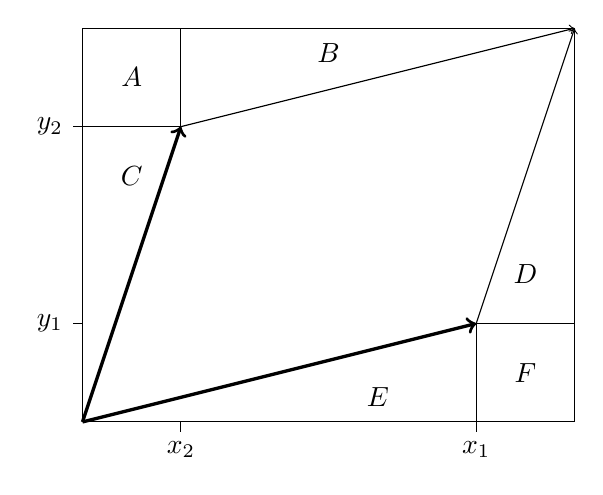
\begin{tikzpicture}[scale=1.25]
\draw (0,0) rectangle (5,4); 
\draw[->,very thick] (0,0) -- (4,1); 
\draw[->,very thick] (0,0) -- (1,3); 
\draw[->] (4,1) -- (5,4); 
\draw[->] (1,3) -- (5,4);
\draw (0,3) -- (1,3) -- (1,4);
\draw (4,0) -- (4,1) -- (5,1);

\draw (1,0) -- (1,-0.1) node [below] {$x_2$}; 
\draw (4,0) -- (4,-0.1) node [below] {$x_1$}; 

\draw (0,1) -- (-0.1,1) node [left] {$y_1$}; 
\draw (0,3) -- (-0.1,3) node [left] {$y_2$}; 

\draw (0.5,2.5) node  {$C$}; 
\draw (0.5,3.5) node {$A$}; 
\draw (2.5,3.75) node {$B$}; 
\draw (3.0,0.25) node {$E$};   
\draw (4.5,0.5) node {$F$};
\draw (4.5,1.5) node {$D$}; 
\end{tikzpicture}
\end{center}

\begin{align*}
\text{area of parallelogram} & = \text{area of enclosing rect} \\
& \qquad - \text{area of rectangle $A$} - \text{area of triangle $B$} \\
& \qquad \cdots - \text{area of rectangle $F$} \\
& = 
(x_1+x_2)(y_1+y_2) - x_2 y_1 - \frac{1}{2} x_1 y_1 \\
& \qquad - \frac{1}{2} x_2 y_2 - \frac{1}{2} x_2 y_2 - \frac{1}{2} x_1 y_1 - x_2 y_1 \\
& = x_1 y_2 - x_2 y_1 
\end{align*}
and note that 
%
\begin{align*}
\begin{vmatrix}
x_1 & x_2 \\
y_1 & y_2 
\end{vmatrix} = x_1 y_2 - x_2 y_1 
\end{align*}

And this result is identical to the determinant seen above.  Again, as noted, the vectors were set up to have a positive area, however in general, one can define the area as the absolute value of the determinant. 


\subsubsection{Transformation of the Vectors and the size of the Parallelogram}

From above, the area of the parallelogram is the 

Consider two vectors in $\mathbb{R}^2$ and rotate them so one is on the $x$-axis.   Also take $\vec{u}$ and multiply it by a factor of $k$ 


\begin{center}
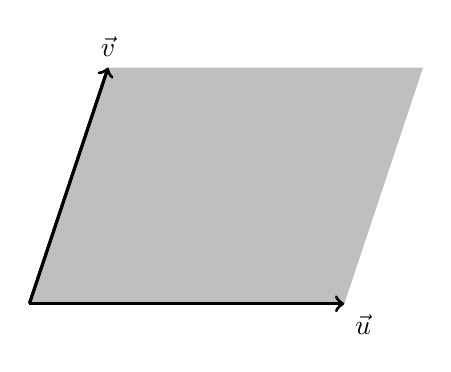
\begin{tikzpicture}
\fill [lightgray] (0,0)-- (4,0) -- (5,3) -- (1,3) -- cycle ;
\draw[->,very thick] (0,0) -- (1,3) node [above] {$\vec{v}$}; 
\draw[->,very thick] (0,0) -- (4,0) node [below right] {$\vec{u}$};  
\end{tikzpicture}
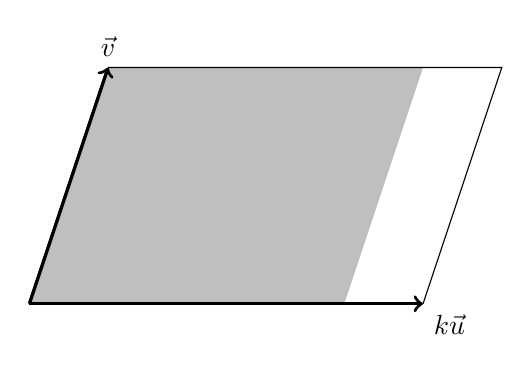
\begin{tikzpicture}
\fill [lightgray] (0,0)-- (4,0) -- (5,3) -- (1,3) -- cycle ;
\draw[->,very thick] (0,0) -- (1,3) node [above] {$\vec{v}$}; 
\draw[->,very thick] (0,0) -- (5,0) node [below right] {$k\vec{u}$}; 
\draw (5,0) -- (6,3) -- (1,3); 
\end{tikzpicture}

\end{center}

From this geometric argument, the area of the parallelogram formed by the vectors $\vec{v}$ and $k\vec{u}$ appears to $k$ times larger.  This is property 3 of Definition \ref{defn:det}.  


Next, let's look at transformation $\vec{u} + k\vec{v}$.  The picture on the left is the original two vectors and that on the right is the transformed vectors (with $k$ about 0.2 in this picture).  The original area and the transformed area are identical in this case since neither the height of the parallelogram nor its width has changed.  

\begin{center}
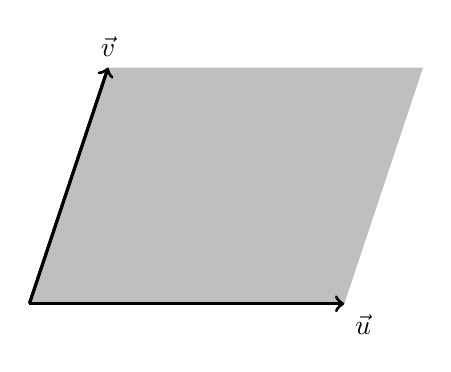
\begin{tikzpicture}
\fill [lightgray] (0,0)-- (4,0) -- (5,3) -- (1,3) -- cycle ;
\draw[->,very thick] (0,0) -- (1,3) node [above] {$\vec{v}$}; 
\draw[->,very thick] (0,0) -- (4,0) node [below right] {$\vec{u}$};  
\end{tikzpicture}
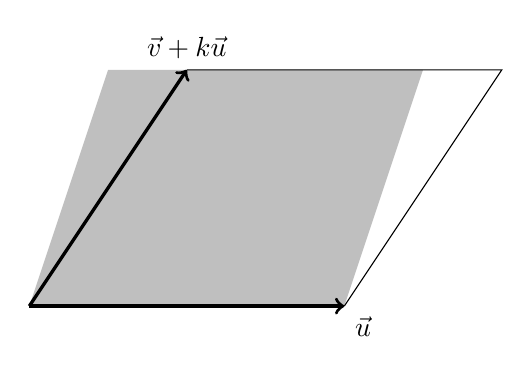
\begin{tikzpicture}
\fill [lightgray] (0,0)-- (4,0) -- (5,3) -- (1,3) -- cycle ;
\draw[->,very thick] (0,0) -- (2,3) node [above] {$\vec{v}+k\vec{u}$}; 
\draw[->,very thick] (0,0) -- (4,0) node [below right] {$\vec{u}$}; 
\draw (4,0) -- (6,3) -- (2,3); 
\end{tikzpicture}
\end{center}

This property shows that replacing a row with a constant times another row plus the current row results in an unchanged area is consistent with property 1 of Definition \ref{defn:det}.  


The other transformation related to the determinant is property 2 of Definition \ref{defn:det} or in other words,  if one switched the order of the vectors (row swaps), that the determinant changes sign.  The area does not change because the area is the absolute value of the determinant.  



\begin{definition}
In $\mathbb{R}^n$, the \textbf{parallelpiped} formed by $\langle \vec{v}_1, \vec{v}_2, \ldots, \vec{v}_n \rangle$ includes the set
%
\begin{align*}
\{ t_1 \vec{v}_1 + t_2 \vec{v}_2 + \cdots + t_n \vec{v}_n\; | \; t_1, t_2, \ldots, t_n \in [0,1] \}
\end{align*}
The \textbf{volume} of the parallelepiped is the absolute value of the determinant of the matrix whose columns are $\vec{v}_1, \vec{v}_2, \ldots, \vec{v}_n$.  
\end{definition}

\begin{example}
Find the volume of the parallelpiped formed by the vectors:
%
\begin{align*}
\begin{bmatrix}
3 \\ 0 \\ 2
\end{bmatrix}, \begin{bmatrix}
-1 \\ 2 \\ 0 
\end{bmatrix}, \begin{bmatrix}
2 \\ 3 \\ 1 
\end{bmatrix}
\end{align*}

\solution

The volume is the absolute value of the determinant of the matrix with these three columns.  We'll use Gauss' method to find the determinant.  

%
\begin{align*}
|A| &= \begin{vmatrix}
3 & -1 & 2 \\
0 & 2 & 3 \\
2 & 0 & 1 
\end{vmatrix} \\
3R_3 \rightarrow R_3 \qquad 
3|A| &= \begin{vmatrix}
3 & -1 & 2 \\
0 & 2 & 3 \\
6 & 0 & 3 
\end{vmatrix} \\
-2 R_1 + R_3 \rightarrow R_3 \qquad
3|A| &= \begin{vmatrix}
3 & -1 & 2 \\
0 & 2 & 3 \\
0 & 2 & -1 
\end{vmatrix} \\
-R_2 + R_3 \rightarrow R_3 \qquad 
3|A| &= \begin{vmatrix}
3 & -1 & 2 \\
0 & 2 & 3 \\
0 & 0 & -4
\end{vmatrix} 
\end{align*}
and multiplying down the diagonal,  $3|A| = -24$, so $|A|=-8$.  This means that the volume is 8 units.  
\end{example}

\vfill \pagebreak
\section{Summary of the basics of  linear algebra}  
\label{sect:linear:algebra:summary}

We finish this chapter with a summarizing theorem about linear algebra.   This covers how much of all of the above concepts are related.   



\begin{theorem} \label{thm:nonsing:matrices}
 Let $A$ be an $n$ by $n$ matrix of real numbers.   The following statements are equivalent:
 
\begin{enumerate}
 \item $|A| \neq 0$ 
 \item The inverse matrix, $A^{-1}$ exists. 
 \item For every vector $\vec{b}$, the equation $A \vec{x}=\vec{b}$ has a unique solution $\vec{x} = A^{-1} \vec{b}$. 
 \item The matrix equation $A \vec{x} = \vec{0}$ has the unique solution $\vec{x} = \vec{0}$.  
 \item The columns of $A$ are linearly independent.
 \item The rows of $A$ are linearly independent.  
 \item The rank of $A$ is $n$.  
 \item The column space of $A$ is $\mathbb{R}^n$ 
 \item The row space of $A$ is $\mathbb{R}^n$.  
 \item The null space of $A$ is $\{\vec{0}\}$ and the nullity is 0.    
 \item The reduced row echelon form of $A$ is $I$, the identity matrix. 
\end{enumerate}
\end{theorem}

\begin{example}
Examine Theorem \ref{thm:nonsing:matrices} using the matrix 

\begin{align*}
A &= \begin{bmatrix}
1 & 0 & 3 \\
0 & 2 & -1 \\
0 & 3 & -1
\end{bmatrix}
\end{align*}

\solution

In this example, we will show all of the equivalent properties directly on the matrix $A$.

\begin{enumerate}
\item First find the determinant.  Using the Laplace expansion method and expanding down the first column
%
\begin{align*}
|A| & = 1 \begin{vmatrix}
2 & -1 \\ 3 & -1 
\end{vmatrix} = 1 (2(-1)-(-1)3) = 1
\end{align*}
which is nonzero. 

\item Next, we'll find the inverse matrix:
%
\begin{align*}
\qquad & \begin{bmatrix}[rrr|rrr]
1 & 0 & 3 & 1 & 0 & 0\\
0 & 2 & -1 & 0 & 1 &0 \\
0 & 3 & -1 & 0 & 0 & 1
\end{bmatrix} \\
-3 R_2 +2 R_3 \rightarrow R_3 \qquad &
\begin{bmatrix}[rrr|rrr]
1 & 0 & 3 & 1 & 0 & 0\\
0 & 2 & -1 & 0 & 1 &0 \\
0 & 0 & 1 & 0 & -3 & 2
\end{bmatrix} \\
\begin{array}{r}
R_3 + R_2 \rightarrow R_2, \\
-3R_3 + R_1 \rightarrow R_1
\end{array} \qquad & 
\begin{bmatrix}[rrr|rrr]
1 & 0 & 0 & 1 & 9 & -6\\
0 & 2 & 0 & 0 & -2 &2 \\
0 & 0 & 1 & 0 & -3 & 2
\end{bmatrix} \\
\frac{1}{2} R_2 \rightarrow R_2 \qquad &
\begin{bmatrix}[rrr|rrr]
1 & 0 & 0 & 1 & 9 & -6\\
0 & 1 & 0 & 0 & -1 & 1 \\
0 & 0 & 1 & 0 & -3 & 2
\end{bmatrix} \\
\end{align*}
and this shows that the inverse matrix is
%
\begin{align*}
A^{-1} &= \begin{bmatrix}
1 & 9 & -6\\
0 & -1 & 1 \\
0 & -3 & 2
\end{bmatrix}
\end{align*}

\item Since the inverse matrix exists, then a unique solution to $A\vec{x}=\vec{b}$ can be found by $\vec{x}=A^{-1}\vec{b}$.  

\item Again, since $A^{-1}$ exists, then 
%
\begin{align*}
\vec{x} & = A^{-1}\vec{0} = \vec{0}
\end{align*}

\item See \#8 below. 
\item See \#9 below. 
\item See \#8 and \#9 below. 

\item The column space is found by row reducing $A^{\intercal}$. 
%
\begin{align*}
A^{\intercal} = &\begin{bmatrix}
1 & 0 & 0 \\
0 & 2 & 3 \\
3 & -1 & -1 
\end{bmatrix} \\
-3 R_1 + R_3 \rightarrow R_3 \qquad & 
\begin{bmatrix}
1 &  0 & 0 \\
0 & 2 & 3\\
0 & -1 & -1 
\end{bmatrix} \\
R_2 + 2 R_3 \rightarrow R_3 \qquad & 
\begin{bmatrix}
1 &  0 & 0 \\
0 & 2 & 3\\
0 & 0 & 1 
\end{bmatrix} \\
\end{align*}
which is now in echelon form and since all nonzero row in a echelon form matrix are linearly independent, this shows \#5.  

Continuing to put this is reduced row echelon form:
\begin{align*}
-3R_3 + R_2 \rightarrow R_2 \qquad & 
\begin{bmatrix}
1 &  0 & 0 \\
0 & 2 & 0\\
0 & 0 & 1 
\end{bmatrix} \\
\frac{1}{2} R_2 \rightarrow R_2 \qquad & 
\begin{bmatrix}
1 &  0 & 0 \\
0 & 1 & 0\\
0 & 0 & 1 
\end{bmatrix} \\
\end{align*}
and this shows that the column space of $A$ is 
%
\begin{align*}
\SPAN(\{ \begin{bmatrix}
1 \\ 0 \\ 0 
\end{bmatrix}, \begin{bmatrix}
0 \\ 1\\0 
\end{bmatrix}, \begin{bmatrix}
 0 \\ 0 \\ 1
\end{bmatrix} \} )
\end{align*}
which is all of $\mathbb{R}^3$.   This also shows that the rank of $A$ is 3. 

\item In a similar manner to \#8, we put $A$ in reduced row echelon form:
%
\begin{align*}
\qquad & \begin{bmatrix}
1 & 0 & 3 \\
0 & 2 & -1 \\
0 & 3 & -1 
\end{bmatrix} \\
-3 R_2 +2 R_3 \rightarrow R_3 \qquad &
\begin{bmatrix}
1 & 0 & 3 \\
0 & 2 & -1\\
0 & 0 & 1 
\end{bmatrix} \\
\begin{array}{r}
R_3 + R_2 \rightarrow R_2, \\
-3R_3 + R_1 \rightarrow R_1
\end{array} \qquad & 
\begin{bmatrix}
1 & 0 & 0 \\
0 & 2 & 0 \\
0 & 0 & 1 
\end{bmatrix} \\
\frac{1}{2} R_2 \rightarrow R_2 \qquad &
\begin{bmatrix}
1 & 0 & 0 \\
0 & 1 & 0 \\
0 & 0 & 1 
\end{bmatrix} \\
\end{align*}

and thus the row space is
%
\begin{align*}
\SPAN(\{ \begin{bmatrix}
1 & 0 & 0 
\end{bmatrix},\begin{bmatrix}
0 & 1 & 0 
\end{bmatrix},\begin{bmatrix}
0 & 0 & 1
\end{bmatrix} \})
\end{align*}
and this is $\mathbb{R}^3$.  In addition, this shows that the rank of $A$ is 3.  
 
 
\item The null space is the set of all $\vec{x}$ such that $A\vec{x}=\vec{0}$, but from \#4, we showed that the only solution to this is $\vec{x}=\vec{0}$.    The nullity is the number of linearly independent vectors in this set which is 0, by definition. 

\item From \#9, we showed that the reduced row echelon form of $A$ is $I$.  
\end{enumerate}

\end{example}


\begin{theorem} \label{thm:sing:matrices}

Let $A$ be an $n \times n$ real matrix.  The following statements are equivalent

\begin{enumerate}
\item $|A|=0$
\item The matrix equation $A \vec{x} = \vec{b}$ has no solution or an infinite number of solutions.
\item The matrix equation $A \vec{x} = \vec{0}$ has a nontrivial solution. 
\item The rank of $A$ is less than $n$.  
\end{enumerate}

\end{theorem}


This theorem will be extremely helpful in finding a certain type of scalar and vector called an eigenvalue and eigenvector.  The following example shows its usefulness. 

\begin{example}
Let 
%
\begin{align*}
A & = \begin{bmatrix}
1 & 0 & 2 \\
0 & -2 & 1 \\
2 & -2 & 5 
\end{bmatrix}
\end{align*}
Show that $A\vec{x} = \vec{0}$ has a nontrivial solution first by using Theorem \ref{thm:sing:matrices} then by directly finding solutions.  

\solution

First, find the determinant by expansion:
%
\begin{align*}
|A| & = 1 \begin{vmatrix}
-2 & 1 \\ -2 & 5 
\end{vmatrix} + 2 \begin{vmatrix}
0 & -2 \\ 2 & -2 
\end{vmatrix} \\
& = (-10-(-2)) + 2 (0-(-4)) = -8 + 8 = 0 
\end{align*}
and therefore by Theorem \ref{thm:sing:matrices}, there is a nontrivial solution to $A \vec{x} = \vec{0}$

Next, we'll solve the matrix equation by Gauss' method. 

\begin{align*}
& \qquad \begin{bmatrix}[rrr|r]
1 & 0 & 2 & 0 \\
0 & -2 & 1 & 0 \\
2 & -2 & 5  & 0 
\end{bmatrix} \\
-2 R_1 + R_3 \rightarrow R_3 
& \qquad \begin{bmatrix}[rrr|r]
1 & 0 & 2 & 0 \\
0 & -2 & 1 & 0 \\
0 & -2 & 1  & 0 
\end{bmatrix} \\
-R_2 + R_3 \rightarrow R_3 
& \qquad \begin{bmatrix}[rrr|r]
1 & 0 & 2 & 0 \\
0 & -2 & 1 & 0 \\
0 & 0 & 0  & 0 
\end{bmatrix} \\
\end{align*} 
The resulting equations are
%
\begin{align*}
x_1 + 2x_3 & = 0 \\
-2x_2 + x_3 & = 0 
\end{align*}
or
\begin{align*}
x_1 & = -2x_3 \\
x_2 & = \frac{1}{2} x_3 
\end{align*}
and the solution set is
%
\begin{align*}
\{ \begin{bmatrix}
-2 \\ 1/2 \\ 1
\end{bmatrix} x_3 \; | \; x_3 \in \mathbb{R} \}
\end{align*}
This shows directly that the matrix equation $A\vec{x}=\vec{0}$ does not have a trivial solution.  
\end{example}

Also notice that the last matrix of Gauss' method showed that the rank was 2 (since there were only 2 nonzero rows).  This was another statement in the theorem.  

